% \documentclass[a4paper,10pt]{article} % or whatever
% \documentclass[letterpaper,10pt]{article} % or whatever
\documentclass{article}

% if you need to pass options to natbib, use, e.g.:
     \PassOptionsToPackage{numbers, compress}{natbib}

\usepackage[preprint]{notes}

\newcommand{\ignore}[1]{}
% to avoid loading the natbib package, add option nonatbib:
\usepackage{dsfont}

% Note: this has been tested using MiKTeX 2.9. If you are getting errors, update your packages.

%%% Packages %%%
%\usepackage{setspace} % Double spaces document. Footnotes,
                      % figures, and tables will still be single spaced, however.
%\doublespacing
%\singlespacing
%\onehalfspacing
% \setstretch{1.5} % set double spacing to 1.5 or anything else.

\usepackage[T1]{fontenc}
\usepackage{amsmath,amssymb,amsfonts,mathrsfs,bm}% Typical maths resource packages
\usepackage{mathtools}
%\let\proof\relax
%\let\endproof\relax
\usepackage{amsthm}
\usepackage{nicefrac}
%\usepackage{cite}
%\let\labelindent\relax
\usepackage[shortlabels]{enumitem}
\usepackage{graphicx}
\usepackage{epstopdf}
\usepackage{url}
\usepackage{colortbl}
\usepackage{booktabs}
\usepackage{multirow}
\usepackage[table,dvipsnames]{xcolor}
\usepackage[normalem]{ulem}
\usepackage{xparse}

%\usepackage{pstricks}
%\usepackage{psfrag}
%\usepackage{syntonly}
%\syntaxonly
%\usepackage[style=base]{caption}
%\captionsetup{
    %format = plain,
    %font = footnotesize,
    %labelfont = sc
%}


\usepackage{array}
\newcolumntype{L}[1]{>{\raggedright\let\newline\\\arraybackslash\hspace{0pt}}m{#1}}
\newcolumntype{C}[1]{>{\centering\let\newline\\\arraybackslash\hspace{0pt}}m{#1}}
\newcolumntype{R}[1]{>{\raggedleft\let\newline\\\arraybackslash\hspace{0pt}}m{#1}}

\makeatletter
\let\MYcaption\@makecaption
\makeatother
\usepackage[font=footnotesize]{subcaption}
\makeatletter
\let\@makecaption\MYcaption
\makeatother


% achieves the functionality of \tag for subequations environment
\makeatletter
\newenvironment{varsubequations}[1]
 {%
  \addtocounter{equation}{-1}%
  \begin{subequations}
  \renewcommand{\theparentequation}{#1}%
  \def\@currentlabel{#1}%
 }
 {%
  \end{subequations}\ignorespacesafterend
 }
\makeatother


\usepackage{glossaries}

\makeatletter
% copy old \gls and \glspl
\let\oldgls\gls
\let\oldglspl\glspl

% define a non space skipping version of \@ifnextchar
\newcommand\fussy@ifnextchar[3]{%
  \let\reserved@d=#1%
  \def\reserved@a{#2}%
  \def\reserved@b{#3}%
  \futurelet\@let@token\fussy@ifnch}
\def\fussy@ifnch{%
  \ifx\@let@token\reserved@d
    \let\reserved@c\reserved@a 
  \else
    \let\reserved@c\reserved@b
  \fi
 \reserved@c}

\renewcommand{\gls}[1]{%
  \oldgls{#1}\fussy@ifnextchar.{\@checkperiod}{\@}}
\renewcommand{\glspl}[1]{%
  \oldglspl{#1}\fussy@ifnextchar.{\@checkperiod}{\@}}

\newcommand{\@checkperiod}[1]{%
  \ifnum\sfcode`\.=\spacefactor\else#1\fi
}
\makeatother

%%%%%%%%%%%%% new add %%%%%%%%%%%%% 
\newcommand{\tb}[1]{\textbf{#1}}


\newacronym{wrt}{w.r.t.}{with respect to}
\newacronym{RHS}{R.H.S.}{right-hand side}
\newacronym{LHS}{L.H.S.}{left-hand side}
\newacronym{iid}{i.i.d.}{independent and identically distributed}
%\newacronym{MIMO}{MIMO}{mulitple-input multiple-output}
%\newacronym{AOA}{AOA}{angle-of-arrival}
%\newacronym{AOD}{AOD}{angle-of-departure}
%\newacronym{LOS}{LOS}{line-of-sight}
%\newacronym{NLOS}{NLOS}{non-line-of-sight}
%\newacronym{TOA}{TOA}{time-of-arrival}
%\newacronym{TDOA}{TDOA}{time-difference-of-arrival}
%\newacronym{RSS}{RSS}{received signal strength}
%\newacronym{GNSS}{GNSS}{Global Navigation Satellite System}
%\newacronym{GSP}{GSP}{graph signal processing}
%\newacronym{ML}{ML}{machine learning}


%put the float package before hyperref and algorithm package after hyperref for hyperref to work correctly with algorithm
\usepackage{float}

\ifx\notloadhyperref\undefined
	\ifx\loadbibentry\undefined
		\usepackage[hidelinks,hypertexnames=false]{hyperref} 
	\else
		\usepackage{bibentry}
		\makeatletter\let\saved@bibitem\@bibitem\makeatother
		\usepackage[hidelinks,hypertexnames=false]{hyperref}
		\makeatletter\let\@bibitem\saved@bibitem\makeatother
	\fi
\else
	\ifx\loadbibentry\undefined
		\relax
	\else
		\usepackage{bibentry}
	\fi
\fi

\usepackage[capitalize]{cleveref}
\crefname{equation}{}{}
\Crefname{equation}{}{}
\crefname{claim}{claim}{claims}
\crefname{step}{step}{steps}
\crefname{line}{line}{lines}
\crefname{condition}{condition}{conditions}
\crefname{dmath}{}{}
\crefname{dseries}{}{}
\crefname{dgroup}{}{}

\crefname{Problem}{Problem}{Problems}
\crefformat{Problem}{Problem~(#2#1#3)}
\crefrangeformat{Problem}{Problems~(#3#1#4) to~(#5#2#6)}

\crefname{Theorem}{Theorem}{Theorems}
\crefname{Corollary}{Corollary}{Corollaries}
\crefname{Proposition}{Proposition}{Propositions}
\crefname{Lemma}{Lemma}{Lemmas}
\crefname{Definition}{Definition}{Definitions}
\crefname{Example}{Example}{Examples}
\crefname{Assumption}{Assumption}{Assumptions}
\crefname{Remark}{Remark}{Remarks}
\crefname{Rem}{Remark}{Remarks}
\crefname{remarks}{Remarks}{Remarks}
\crefname{Appendix}{Appendix}{Appendices}
\crefname{Supplement}{Supplement}{Supplements}
\crefname{Exercise}{Exercise}{Exercises}
\crefname{Theorem_A}{Theorem}{Theorems}
\crefname{Corollary_A}{Corollary}{Corollaries}
\crefname{Proposition_A}{Proposition}{Propositions}
\crefname{Lemma_A}{Lemma}{Lemmas}
\crefname{Definition_A}{Definition}{Definitions}
\crefname{rema}{Remark}{Remarks}
\crefname{exma}{Example}{Examples}

\usepackage{crossreftools}
\ifx\notloadhyperref\undefined
	\pdfstringdefDisableCommands{%
			\let\Cref\crtCref
			\let\cref\crtcref
	}
\else
	\relax
\fi

\usepackage{algorithm,algorithmic}
\renewcommand{\algorithmicrequire}{\textbf{Input:}}
\renewcommand{\algorithmicensure}{\textbf{Output:}}

%may cause conflict with some packages like tikz, include manually if desired
%load after hyperref
\ifx\loadbreqn\undefined
	\relax
\else
	\usepackage{breqn} 
\fi



%%%%%%%%%%%%%%%%%%%%%%%%%%%%%%%%%%%%%%%%%%%%%%%%


\interdisplaylinepenalty=2500   % To restore IEEEtran ability to automatically break
                                % within multiline equations, when using amsmath.

%%%%%%%%%%%%%%%%%%%%%%%%%%%%%%%%%%%%%%%%

%Theorem declarations

\ifx\renewtheorem\undefined
% for use in main body
\ifx\useTheoremCounter\undefined
\newtheorem{Theorem}{Theorem}
\newtheorem{Corollary}{Corollary}
\newtheorem{Proposition}{Proposition}
\newtheorem{Lemma}{Lemma}
\else
\newtheorem{Theorem}{Theorem}
\newtheorem{Corollary}[theorem]{Corollary}
\newtheorem{Proposition}[theorem]{Proposition}
\fi

\newtheorem{Definition}{Definition}
\newtheorem{Example}{Example}
\newtheorem{Remark}{Remark}
\newtheorem{Assumption}{Assumption}
\newtheorem{Exercise}{Exercise}

% for use in the appendix
\newtheorem{Theorem_A}{Theorem}[section]
\newtheorem{Corollary_A}{Corollary}[section]
\newtheorem{Proposition_A}{Proposition}[section]
\newtheorem{Lemma_A}{Lemma}[section]
\newtheorem{Definition_A}{Definition}[section]
\fi

\usepackage{amsmath}
\numberwithin{equation}{section} % or whatever you prefer
% \swapnumbers % I prefer this
% \theoremstyle{plain}
\newtheorem{thma}[equation]{Theorem}
\newtheorem{propa}[equation]{Proposition}
\newtheorem{lema}[equation]{Lemma}
\newtheorem{defa}[equation]{Definition}
\newtheorem{cora}[equation]{Corollary}
\newtheorem{Lemma_AA}{Lemma}[section]
\newtheorem{rema}[equation]{Remark}
\newtheorem{exma}[equation]{Example}
\newcommand{\ml}[1]{\begin{multlined}#1\end{multlined}}
\newcommand{\nn}{\nonumber\\ }


% Remarks
\theoremstyle{remark}
\newtheorem{Rem}{Remark}
\theoremstyle{plain}

\newenvironment{remarks}{
	\begin{list}{\textit{Remark} \arabic{Rem}:~}{
    \setcounter{enumi}{\value{Rem}}
    \usecounter{Rem}
    \setcounter{Rem}{\value{enumi}}
    \setlength\labelwidth{0in}
    \setlength\labelsep{0in}
    \setlength\leftmargin{0in}
    \setlength\listparindent{0in}
    \setlength\itemindent{15pt}
		}
}{
	\end{list}
}


% Special Headings
%\newtheorem*{Prop1}{Proposition 1} %needs amsthm

%\newtheoremstyle{nonum}{}{}{\itshape}{}{\bfseries}{.}{ }{#1 (\mdseries #3)}
%\theoremstyle{nonum}
%\newtheorem{Example**}{Example 1}

\newcommand{\EndExample}{{$\square$}}
%\renewcommand{\QED}{\QEDopen} % changes end of proof box to open box.

\newcommand{\qednew}{\nobreak \ifvmode \relax \else
      \ifdim\lastskip<1.5em \hskip-\lastskip
      \hskip1.5em plus0em minus0.5em \fi \nobreak
      \vrule height0.75em width0.5em depth0.25em\fi}


%\newcommand{\em}[1]{\emph{#1}}

% Move down subscripts for some symbols like \chi
\NewDocumentCommand{\movedownsub}{e{^_}}{%
  \IfNoValueTF{#1}{%
    \IfNoValueF{#2}{^{}}% neither ^ nor _, do nothing; if no ^ but _, add ^{}
  }{%
    ^{#1}% add superscript if present
  }%
  \IfNoValueF{#2}{_{#2}}% add subscript if present
}



%Number sets
\newcommand{\Real}{\mathbb{R}}
\newcommand{\Nat}{\mathbb{N}}
\newcommand{\Rat}{\mathbb{Q}}
\newcommand{\Complex}{\mathbb{C}}

% imaginary number i
\newcommand{\iu}{\mathfrak{i}\mkern1mu}


% Calligraphic stuff
\newcommand{\calA}{\mathcal{A}}
\newcommand{\calB}{\mathcal{B}}
\newcommand{\calC}{\mathcal{C}}
\newcommand{\calD}{\mathcal{D}}
\newcommand{\calE}{\mathcal{E}}
\newcommand{\calF}{\mathcal{F}}
\newcommand{\calG}{\mathcal{G}}
\newcommand{\calH}{\mathcal{H}}
\newcommand{\calI}{\mathcal{I}}
\newcommand{\calJ}{\mathcal{J}}
\newcommand{\calK}{\mathcal{K}}
\newcommand{\calL}{\mathcal{L}}
\newcommand{\calM}{\mathcal{M}}
\newcommand{\calN}{\mathcal{N}}
\newcommand{\calO}{\mathcal{O}}
\newcommand{\calP}{\mathcal{P}}
\newcommand{\calQ}{\mathcal{Q}}
\newcommand{\calR}{\mathcal{R}}
\newcommand{\calS}{\mathcal{S}}
\newcommand{\calT}{\mathcal{T}}
\newcommand{\calU}{\mathcal{U}}
\newcommand{\calV}{\mathcal{V}}
\newcommand{\calW}{\mathcal{W}}
\newcommand{\calX}{\mathcal{X}}
\newcommand{\calY}{\mathcal{Y}}
\newcommand{\calZ}{\mathcal{Z}}

% Boldface stuff
\newcommand{\ba}{\mathbf{a}}
\newcommand{\bA}{\mathbf{A}}
\newcommand{\bb}{\mathbf{b}}
\newcommand{\bB}{\mathbf{B}}
\newcommand{\bc}{\mathbf{c}}
\newcommand{\bC}{\mathbf{C}}
\newcommand{\bd}{\mathbf{d}}
\newcommand{\bD}{\mathbf{D}}
\newcommand{\be}{\mathbf{e}}
\newcommand{\bE}{\mathbf{E}}
\newcommand{\boldf}{\mathbf{f}}
\newcommand{\bF}{\mathbf{F}}
\newcommand{\bg}{\mathbf{g}}
\newcommand{\bG}{\mathbf{G}}
\newcommand{\bh}{\mathbf{h}}
\newcommand{\bH}{\mathbf{H}}
\newcommand{\bi}{\mathbf{i}}
\newcommand{\bI}{\mathbf{I}}
\newcommand{\bj}{\mathbf{j}}
\newcommand{\bJ}{\mathbf{J}}
\newcommand{\bk}{\mathbf{k}}
\newcommand{\bK}{\mathbf{K}}
\newcommand{\bl}{\mathbf{l}}
\newcommand{\bL}{\mathbf{L}}
\newcommand{\boldm}{\mathbf{m}}
\newcommand{\bM}{\mathbf{M}}
\newcommand{\bn}{\mathbf{n}}
\newcommand{\bN}{\mathbf{N}}
\newcommand{\bo}{\mathbf{o}}
\newcommand{\bO}{\mathbf{O}}
\newcommand{\bp}{\mathbf{p}}
\newcommand{\bP}{\mathbf{P}}
\newcommand{\bq}{\mathbf{q}}
\newcommand{\bQ}{\mathbf{Q}}
\newcommand{\br}{\mathbf{r}}
\newcommand{\bR}{\mathbf{R}}
\newcommand{\bs}{\mathbf{s}}
\newcommand{\bS}{\mathbf{S}}
\newcommand{\bt}{\mathbf{t}}
\newcommand{\bT}{\mathbf{T}}
\newcommand{\bu}{\mathbf{u}}
\newcommand{\bU}{\mathbf{U}}
\newcommand{\bv}{\mathbf{v}}
\newcommand{\bV}{\mathbf{V}}
\newcommand{\bw}{\mathbf{w}}
\newcommand{\bW}{\mathbf{W}}
\newcommand{\bx}{\mathbf{x}}
\newcommand{\bX}{\mathbf{X}}
\newcommand{\by}{\mathbf{y}}
\newcommand{\bY}{\mathbf{Y}}
\newcommand{\bz}{\mathbf{z}}
\newcommand{\bZ}{\mathbf{Z}}


\newcommand{\mba}{\bm{a}}
\newcommand{\mbA}{\bm{A}}
\newcommand{\mbb}{\bm{b}}
\newcommand{\mbB}{\bm{B}}
\newcommand{\mbc}{\bm{c}}
\newcommand{\mbC}{\bm{C}}
\newcommand{\mbd}{\bm{d}}
\newcommand{\mbD}{\bm{D}}
\newcommand{\mbe}{\bm{e}}
\newcommand{\mbE}{\bm{E}}
\newcommand{\mbf}{\bm{f}}
\newcommand{\mbF}{\bm{F}}
\newcommand{\mbg}{\bm{g}}
\newcommand{\mbG}{\bm{G}}
\newcommand{\mbh}{\bm{h}}
\newcommand{\mbH}{\bm{H}}
\newcommand{\mbi}{\bm{i}}
\newcommand{\mbI}{\bm{I}}
\newcommand{\mbj}{\bm{j}}
\newcommand{\mbJ}{\bm{J}}
\newcommand{\mbk}{\bm{k}}
\newcommand{\mbK}{\bm{K}}
\newcommand{\mbl}{\bm{l}}
\newcommand{\mbL}{\bm{L}}
\newcommand{\mbm}{\bm{m}}
\newcommand{\mbM}{\bm{M}}
\newcommand{\mbn}{\bm{n}}
\newcommand{\mbN}{\bm{N}}
\newcommand{\mbo}{\bm{o}}
\newcommand{\mbO}{\bm{O}}
\newcommand{\mbp}{\bm{p}}
\newcommand{\mbP}{\bm{P}}
\newcommand{\mbq}{\bm{q}}
\newcommand{\mbQ}{\bm{Q}}
\newcommand{\mbr}{\bm{r}}
\newcommand{\mbR}{\bm{R}}
\newcommand{\mbs}{\bm{s}}
\newcommand{\mbS}{\bm{S}}
\newcommand{\mbt}{\bm{t}}
\newcommand{\mbT}{\bm{T}}
\newcommand{\mbu}{\bm{u}}
\newcommand{\mbU}{\bm{U}}
\newcommand{\mbv}{\bm{v}}
\newcommand{\mbV}{\bm{V}}
\newcommand{\mbw}{\bm{w}}
\newcommand{\mbW}{\bm{W}}
\newcommand{\mbx}{\bm{x}}
\newcommand{\mbX}{\bm{X}}
\newcommand{\mby}{\bm{y}}
\newcommand{\mbY}{\bm{Y}}
\newcommand{\mbz}{\bm{z}}
\newcommand{\mbZ}{\bm{Z}}

% Numbers bb font
\newcommand{\bbA}{\mathbb{A}}
\newcommand{\bbB}{\mathbb{B}}
\newcommand{\bbC}{\mathbb{C}}
\newcommand{\bbD}{\mathbb{D}}
\newcommand{\bbE}{\mathbb{E}}
\newcommand{\bbF}{\mathbb{F}}
\newcommand{\bbG}{\mathbb{G}}
\newcommand{\bbH}{\mathbb{H}}
\newcommand{\bbI}{\mathbb{I}}
\newcommand{\bbJ}{\mathbb{J}}
\newcommand{\bbK}{\mathbb{K}}
\newcommand{\bbL}{\mathbb{L}}
\newcommand{\bbM}{\mathbb{M}}
\newcommand{\bbN}{\mathbb{N}}
\newcommand{\bbO}{\mathbb{O}}
\newcommand{\bbP}{\mathbb{P}}
\newcommand{\bbQ}{\mathbb{Q}}
\newcommand{\bbR}{\mathbb{R}}
\newcommand{\bbS}{\mathbb{S}}
\newcommand{\bbT}{\mathbb{T}}
\newcommand{\bbU}{\mathbb{U}}
\newcommand{\bbV}{\mathbb{V}}
\newcommand{\bbW}{\mathbb{W}}
\newcommand{\bbX}{\mathbb{X}}
\newcommand{\bbY}{\mathbb{Y}}
\newcommand{\bbZ}{\mathbb{Z}}

% Mathfrak font
\newcommand{\frakA}{\mathfrak{A}}
\newcommand{\frakB}{\mathfrak{B}}
\newcommand{\frakC}{\mathfrak{C}}
\newcommand{\frakD}{\mathfrak{D}}
\newcommand{\frakE}{\mathfrak{E}}
\newcommand{\frakF}{\mathfrak{F}}
\newcommand{\frakG}{\mathfrak{G}}
\newcommand{\frakH}{\mathfrak{H}}
\newcommand{\frakI}{\mathfrak{I}}
\newcommand{\frakJ}{\mathfrak{J}}
\newcommand{\frakK}{\mathfrak{K}}
\newcommand{\frakL}{\mathfrak{L}}
\newcommand{\frakM}{\mathfrak{M}}
\newcommand{\frakN}{\mathfrak{N}}
\newcommand{\frakO}{\mathfrak{O}}
\newcommand{\frakP}{\mathfrak{P}}
\newcommand{\frakQ}{\mathfrak{Q}}
\newcommand{\frakR}{\mathfrak{R}}
\newcommand{\frakS}{\mathfrak{S}}
\newcommand{\frakT}{\mathfrak{T}}
\newcommand{\frakU}{\mathfrak{U}}
\newcommand{\frakV}{\mathfrak{V}}
\newcommand{\frakW}{\mathfrak{W}}
\newcommand{\frakX}{\mathfrak{X}}
\newcommand{\frakY}{\mathfrak{Y}}
\newcommand{\frakZ}{\mathfrak{Z}}

% Mathscr
\newcommand{\scA}{\mathscr{A}}
\newcommand{\scB}{\mathscr{B}}
\newcommand{\scC}{\mathscr{C}}
\newcommand{\scD}{\mathscr{D}}
\newcommand{\scE}{\mathscr{E}}
\newcommand{\scF}{\mathscr{F}}
\newcommand{\scG}{\mathscr{G}}
\newcommand{\scH}{\mathscr{H}}
\newcommand{\scI}{\mathscr{I}}
\newcommand{\scJ}{\mathscr{J}}
\newcommand{\scK}{\mathscr{K}}
\newcommand{\scL}{\mathscr{L}}
\newcommand{\scM}{\mathscr{M}}
\newcommand{\scN}{\mathscr{N}}
\newcommand{\scO}{\mathscr{O}}
\newcommand{\scP}{\mathscr{P}}
\newcommand{\scQ}{\mathscr{Q}}
\newcommand{\scR}{\mathscr{R}}
\newcommand{\scS}{\mathscr{S}}
\newcommand{\scT}{\mathscr{T}}
\newcommand{\scU}{\mathscr{U}}
\newcommand{\scV}{\mathscr{V}}
\newcommand{\scW}{\mathscr{W}}
\newcommand{\scX}{\mathscr{X}}
\newcommand{\scY}{\mathscr{Y}}
\newcommand{\scZ}{\mathscr{Z}}


% define some useful uppercase Greek letters in regular and bold sf
\DeclareSymbolFont{bsfletters}{OT1}{cmss}{bx}{n}
\DeclareSymbolFont{ssfletters}{OT1}{cmss}{m}{n}
\DeclareMathSymbol{\bsfGamma}{0}{bsfletters}{'000}
\DeclareMathSymbol{\ssfGamma}{0}{ssfletters}{'000}
\DeclareMathSymbol{\bsfDelta}{0}{bsfletters}{'001}
\DeclareMathSymbol{\ssfDelta}{0}{ssfletters}{'001}
\DeclareMathSymbol{\bsfTheta}{0}{bsfletters}{'002}
\DeclareMathSymbol{\ssfTheta}{0}{ssfletters}{'002}
\DeclareMathSymbol{\bsfLambda}{0}{bsfletters}{'003}
\DeclareMathSymbol{\ssfLambda}{0}{ssfletters}{'003}
\DeclareMathSymbol{\bsfXi}{0}{bsfletters}{'004}
\DeclareMathSymbol{\ssfXi}{0}{ssfletters}{'004}
\DeclareMathSymbol{\bsfPi}{0}{bsfletters}{'005}
\DeclareMathSymbol{\ssfPi}{0}{ssfletters}{'005}
\DeclareMathSymbol{\bsfSigma}{0}{bsfletters}{'006}
\DeclareMathSymbol{\ssfSigma}{0}{ssfletters}{'006}
\DeclareMathSymbol{\bsfUpsilon}{0}{bsfletters}{'007}
\DeclareMathSymbol{\ssfUpsilon}{0}{ssfletters}{'007}
\DeclareMathSymbol{\bsfPhi}{0}{bsfletters}{'010}
\DeclareMathSymbol{\ssfPhi}{0}{ssfletters}{'010}
\DeclareMathSymbol{\bsfPsi}{0}{bsfletters}{'011}
\DeclareMathSymbol{\ssfPsi}{0}{ssfletters}{'011}
\DeclareMathSymbol{\bsfOmega}{0}{bsfletters}{'012}
\DeclareMathSymbol{\ssfOmega}{0}{ssfletters}{'012}


% Bold greek
\newcommand{\balpha}{\bm{\alpha}}
\newcommand{\bbeta}{\bm{\beta}}
\newcommand{\bgamma}{\bm{\gamma}}
\newcommand{\bdelta}{\bm{\delta}}
\newcommand{\btheta}{\bm{\theta}}
\newcommand{\bmu}{\bm{\mu}}
\newcommand{\bnu}{\bm{\nu}}
\newcommand{\btau}{\bm{\tau}}
\newcommand{\bpi}{\bm{\pi}}
\newcommand{\bepsilon}{\bm{\epsilon}}
\newcommand{\veps}{\varepsilon}
\newcommand{\bvarepsilon}{\bm{\varepsilon}}
\newcommand{\bsigma}{\bm{\sigma}}
\newcommand{\bvarsigma}{\bm{\varsigma}}
\newcommand{\bzeta}{\bm{\zeta}}
\newcommand{\bmeta}{\bm{\eta}}
\newcommand{\bkappa}{\bm{\kappa}}
\newcommand{\bchi}{\bm{\latexchi}\movedownsub}
\newcommand{\bphi}{\bm{\phi}}
\newcommand{\bpsi}{\bm{\psi}}
\newcommand{\bomega}{\bm{\omega}}
\newcommand{\bxi}{\bm{\xi}}
\newcommand{\blambda}{\bm{\lambda}}
\newcommand{\brho}{\bm{\rho}}

\newcommand{\bGamma}{\bm{\Gamma}}
\newcommand{\bLambda}{\bm{\Lambda}}
\newcommand{\bSigma	}{\bm{\Sigma}}
\newcommand{\bPsi}{\bm{\Psi}}
\newcommand{\bDelta}{\bm{\Delta}}
\newcommand{\bXi}{\bm{\Xi}}
\newcommand{\bUpsilon}{\bm{\Upsilon}}
\newcommand{\bOmega}{\bm{\Omega}}
\newcommand{\bPhi}{\bm{\Phi}}
\newcommand{\bPi}{\bm{\Pi}}
\newcommand{\bTheta}{\bm{\Theta}}

\newcommand{\talpha}{\widetilde{\alpha}}
\newcommand{\tbeta}{\widetilde{\beta}}
\newcommand{\tgamma}{\widetilde{\gamma}}
\newcommand{\tdelta}{\widetilde{\delta}}
\newcommand{\ttheta}{\widetilde{\theta}}
\newcommand{\tmu}{\widetilde{\mu}}
\newcommand{\tnu}{\widetilde{\nu}}
\newcommand{\ttau}{\widetilde{\tau}}
\newcommand{\tpi}{\widetilde{\pi}}
\newcommand{\tepsilon}{\widetilde{\epsilon}}
\newcommand{\tvarepsilon}{\widetilde{\varepsilon}}
\newcommand{\tsigma}{\widetilde{\sigma}}
\newcommand{\tzeta}{\widetilde{\zeta}}
\newcommand{\tmeta}{\widetilde{\eta}}
\newcommand{\tkappa}{\widetilde{\kappa}}
\newcommand{\tchi}{\widetilde{\latexchi}\movedownsub}
\newcommand{\tphi}{\widetilde{\phi}}
\newcommand{\tpsi}{\widetilde{\psi}}
\newcommand{\tomega}{\widetilde{\omega}}
\newcommand{\txi}{\widetilde{\xi}}
\newcommand{\tlambda}{\widetilde{\lambda}}
\newcommand{\trho}{\widetilde{\rho}}

\newcommand{\tbAlpha}{\widetilde{\bAlpha}}
\newcommand{\tbBeta}{\widetilde{\bBeta}}
\newcommand{\tbGamma}{\widetilde{\bGamma}}
\newcommand{\tbDelta}{\widetilde{\bDelta}}
\newcommand{\tbTheta}{\widetilde{\bTheta}}
\newcommand{\tbPi}{\widetilde{\bPi}}
\newcommand{\tbSigma}{\widetilde{\bSigma}}
\newcommand{\tbPhi}{\widetilde{\bPhi}}
\newcommand{\tbPsi}{\widetilde{\bPsi}}
\newcommand{\tbOmega}{\widetilde{\bOmega}}
\newcommand{\tbXi}{\widetilde{\bXi}}
\newcommand{\tbLambda}{\widetilde{\bLambda}}

\newcommand{\halpha}{\widehat{\alpha}}
\newcommand{\hbeta}{\widehat{\beta}}
\newcommand{\hgamma}{\widehat{\gamma}}
\newcommand{\hdelta}{\widehat{\delta}}
\newcommand{\htheta}{\widehat{\theta}}
\newcommand{\hmu}{\widehat{\mu}}
\newcommand{\hnu}{\widehat{\nu}}
\newcommand{\htau}{\widehat{\tau}}
\newcommand{\hpi}{\widehat{\pi}}
\newcommand{\hepsilon}{\widehat{\epsilon}}
\newcommand{\hvarepsilon}{\widehat{\varepsilon}}
\newcommand{\hsigma}{\widehat{\sigma}}
\newcommand{\hzeta}{\widehat{\zeta}}
\newcommand{\hmeta}{\widehat{\eta}}
\newcommand{\hkappa}{\widehat{\kappa}}
\newcommand{\hchi}{\widehat{\latexchi}\movedownsub}
\newcommand{\hphi}{\widehat{\phi}}
\newcommand{\barbPhi}{\bar{\bPhi}}
\newcommand{\hpsi}{\widehat{\psi}}
\newcommand{\homega}{\widehat{\omega}}
\newcommand{\hxi}{\widehat{\xi}}
\newcommand{\hlambda}{\widehat{\lambda}}
\newcommand{\hrho}{\widehat{\rho}}


%MathOperator
\DeclareMathOperator*{\argmax}{arg\,max}
\DeclareMathOperator*{\argmin}{arg\,min}
\DeclareMathOperator*{\argsup}{arg\,sup}
\DeclareMathOperator*{\arginf}{arg\,inf}
\DeclareMathOperator*{\minimize}{minimize}
\DeclareMathOperator*{\maximize}{maximize}
\DeclareMathOperator{\st}{s.t.\ }
%\DeclareMathOperator{\st}{subject\,\,to}
\DeclareMathOperator{\as}{a.s.}
\DeclareMathOperator{\diag}{diag}
\DeclareMathOperator{\cum}{cum}
\DeclareMathOperator{\sgn}{sgn}
\DeclareMathOperator{\tr}{tr}
\DeclareMathOperator{\Tr}{Tr}
\DeclareMathOperator{\spn}{span}
\DeclareMathOperator{\supp}{supp}
\DeclareMathOperator{\adj}{adj}
\DeclareMathOperator{\var}{var}
\DeclareMathOperator{\Vol}{Vol}
\DeclareMathOperator{\cov}{cov}
\DeclareMathOperator{\corr}{corr}
\DeclareMathOperator{\sech}{sech}
\DeclareMathOperator{\sinc}{sinc}
\DeclareMathOperator{\rank}{rank}
\DeclareMathOperator{\poly}{poly}
\DeclareMathOperator{\vect}{vec}
\DeclareMathOperator{\conv}{conv}
\DeclareMathOperator*{\lms}{l.i.m.\,}
\DeclareMathOperator*{\esssup}{ess\,sup}
\DeclareMathOperator*{\essinf}{ess\,inf}
\DeclareMathOperator{\sign}{sign}
\DeclareMathOperator{\eig}{eig}
\DeclareMathOperator{\Ima}{Im}
\DeclareMathOperator{\Mod}{mod}

%Paired delimiters
\DeclarePairedDelimiter\abs{\lvert}{\rvert}
\DeclarePairedDelimiter\parens{(}{)}
\DeclarePairedDelimiter\brk{[}{]}
\DeclarePairedDelimiter\braces{\{}{\}}
\DeclarePairedDelimiter\angles{\langle}{\rangle}
\DeclarePairedDelimiterX\ip[2]{\langle}{\rangle}{#1,#2}
\DeclarePairedDelimiterX\norm[1]{\lVert}{\rVert}{#1}
\DeclarePairedDelimiterXPP\col[1]{\operatorname{col}}{\{}{\}}{}{#1} % column vector
\DeclarePairedDelimiterXPP\row[1]{\operatorname{row}}{\{}{\}}{}{#1} % row vector
\DeclarePairedDelimiterXPP\erf[1]{\operatorname{erf}}{(}{)}{}{#1}
\DeclarePairedDelimiterXPP\erfc[1]{\operatorname{erfc}}{(}{)}{}{#1}
\DeclarePairedDelimiterXPP\op[2]{\operatorname{#1}}{(}{)}{}{#2} % general operator


% Math relations
\newcommand{\convp}{\stackrel{\mathrm{p}}{\longrightarrow}}
\newcommand{\convas}{\stackrel{\mathrm{a.s.}}{\longrightarrow}}
\newcommand{\convd}{\stackrel{\mathrm{d}}{\longrightarrow}}
\newcommand{\convD}{\stackrel{\mathrm{D}}{\longrightarrow}}

\newcommand{\dotleq}{\stackrel{.}{\leq}}
\newcommand{\dotlt}{\stackrel{.}{<}}
\newcommand{\dotgeq}{\stackrel{.}{\geq}}
\newcommand{\dotgt}{\stackrel{.}{>}}
\newcommand{\dotdoteq}{\stackrel{\,..}{=}}

\newcommand{\eqa}[1]{\stackrel{#1}{=}}
\newcommand{\ed}{\eqa{\mathrm{d}}}
\newcommand{\lea}[1]{\stackrel{#1}{\le}}
\newcommand{\gea}[1]{\stackrel{#1}{\ge}}

\newcommand{\T}{^{\intercal}}% transpose notation
\newcommand{\setcomp}{^{\mathsf{c}}} %set complement
\newcommand{\ud}{\,\mathrm{d}} % for integrals like \int f(x) \ud x
\newcommand{\Id}{\mathrm{Id}} % identity function
\newcommand{\Bigmid}{{\ \Big| \ }}
\newcommand{\bzero}{\bm{0}}
\newcommand{\bone}{\bm{1}}

% Math functions
\newcommand{\indicator}[1]{{\bf 1}_{\braces*{#1}}}
\newcommand{\indicatore}[1]{{\bf 1}_{#1}}
\newcommand{\indicate}[1]{{\bf 1}\braces*{#1}}
\newcommand{\ofrac}[1]{{\frac{1}{#1}}}
\newcommand{\odfrac}[1]{{\dfrac{1}{#1}}}
\newcommand{\ddfrac}[2]{{\dfrac{\mathrm{d} {#1}}{\mathrm{d} {#2}}}}
\newcommand{\ppfrac}[2]{\dfrac{\partial {#1}}{\partial {#2}}}
\newcommand{\tc}[1]{^{(#1)}}
\newcommand{\ceil}[1]{\left\lceil{#1}\right\rceil}
\newcommand{\floor}[1]{\left\lfloor{#1}\right\rfloor}
\newcommand{\trace}[1]{{\Tr\left( #1 \right)}}

\newcommand{\KLD}[2]{{D({#1}\, \|\, {#2})}}
\newcommand{\Lh}[1]{\ell_{#1}}
\newcommand{\LLh}[1]{\log{\Lh{#1}}}
\newcommand{\cond}[2]{\left. {#1}\, \middle| \, {#2} \right.}


% just to make sure it exists
\providecommand\given{}
% can be useful to refer to this outside \set
\newcommand\SetSymbol[2][]{%
\nonscript\, #1#2
\allowbreak
\nonscript\,
\mathopen{}}

\DeclarePairedDelimiterX\Set[2]\{\}{%
\renewcommand\given{\SetSymbol[\delimsize]{#1}}
#2
}
\DeclarePairedDelimiterX\Setc[1]\{\}{%
\renewcommand\given{\SetSymbol{:}}
#1
}

% \set{x \given f(x)=1} gives \{x : f(x)=1\}
% \set[\vert]{x \given f(x)=1} gives \{x \vert f(x)=1\}
% Starred version uses \left and \right
\NewDocumentCommand\set{s o m}{%
	\IfBooleanTF#1%
	{\IfValueTF{#2}{\Set*{#2}{#3}}{\Setc*{#3}}}%
	{\IfValueTF{#2}{\Set{#2}{#3}}{\Setc{#3}}}%
}

%\NewDocumentCommand\set{s m t| m}{%
  %\IfBooleanTF#1%
	%{\left\{\, #2\mathrel{} \IfBooleanTF{#3}{\middle|}{:}\mathrel{}  #4\, \right\}}%
  %{\{\, #2 \IfBooleanTF{#3}{\mid}{\mathrel{} : \mathrel{}} #4\, \}}% 
%}

\NewDocumentCommand{\evalat}{s O{\big} m m}{%
  \IfBooleanTF{#1}
   {{\left. #3 \right|_{#4}}}
   {{#3#2|_{#4}}}%
}

\NewDocumentCommand \ifcond {m m} {%
	{#1} %
	\IfValueT{#2}{\, \middle|\, {#2}}%
}

%\newcommand\argProtect[1]{\def\ProcessedArgument{{#1}}}
	
% Allows the use of 
% \P : \mathbb{P}
% \P(X) : \mathbb{P}\left({X}\right)
% \P_{p}(X) or \P{p}(X) : \mathbb{P}_{p}\left({X}\right)
% \P(X @| Y) or \P(X){Y} : \mathbb{P}\left({X}\, \middle| \, {Y}\right). 
% \P_{p}(X @| Y) or \P{p}(X){Y} : \mathbb{P}_{p}\left({X}\, \middle| \, {Y}\right)
% Caveats: Iterated expressions do not work well with \P(X @| Y) notation
% \P(\P(X @| Y) @| Z) does not work, use \P({\P(X @| Y)} @| Z) or \P(\P(X){Y} @| Z)
% \P(\P(X @| Y)) does not work, use \P( {\P(X @| Y)} )
\DeclareDocumentCommand \P {e{_} g >{\SplitArgument{ 1 }{ @| }}d() g } {%
	\mathbb{P}%
	\IfValueTF{#1}{_{#1}}
		{\IfValueT{#2}{_{#2}}}%
	\IfValueT{#3}{\left(\ifcond#3}%
	\IfValueT{#4}{\, \middle|\, {#4}}%
	\IfValueT{#3}{\right)}%
}

% Allows the use of 
% \E : \mathbb{E}
% \E[X] : \mathbb{E}\left[{X}\right]
% \E_{p}[X] or \E{p}[X] : \mathbb{E}_{p}\left[{X}\right]
% \E[X @| Y] or \E[X]{Y} : \mathbb{E}\left[{X}\, \middle| \, {Y}\right]. 
% \E_{p}[X @| Y] or \E{p}[X]{Y} : \mathbb{E}_{p}\left[{X}\, \middle| \, {Y}\right]
% Caveats: Iterated expressions do not work well with \E[X @| Y] notation
% \E[\E[X @| Y] @| Z] does not work, use \E[{\E[X @| Y]} @| Z] or \E[\E[X]{Y} @| Z]
% \E[\E[X @| Y]] does not work, use \E[ {\E[X @| Y]} ]
\DeclareDocumentCommand \E {e{_} g >{\SplitArgument{ 1 }{ @| }}o g } {%
	\mathbb{E}%
	\IfValueTF{#1}{_{#1}}
		{\IfValueT{#2}{_{#2}}}%
	\IfValueT{#3}{\left[\ifcond#3}%
	\IfValueT{#4}{\, \middle|\, {#4}}%
	\IfValueT{#3}{\right]}%
}

\def\independenT#1#2{\mathrel{\rlap{$#1#2$}\mkern5mu{#1#2}}}
\newcommand\independent{\protect\mathpalette{\protect\independenT}{\perp}}
\newcommand{\Bern}[1]{\mathrm{Bern}\left(#1\right)}
\newcommand{\Unif}[1]{\mathrm{Unif}\left(#1\right)}
\newcommand{\Dir}[1]{\mathrm{Dir}\left(#1\right)}
\newcommand{\Cat}[1]{\mathrm{Cat}\left(#1\right)}
\newcommand{\N}[2]{{\calN\left({#1},\, {#2}\right)}}
\newcommand{\Beta}[2]{{\calB e\left({#1},\, {#2}\right)}}


\let\oldforall\forall
\renewcommand{\forall}{\oldforall \, }

\let\oldexist\exists
\renewcommand{\exists}{\oldexist \: }

\newcommand\existu{\oldexist! \: }


% Figures
\renewcommand{\figurename}{Fig.}
\newcommand{\figref}[1]{\figurename~\ref{#1}}
\graphicspath{{./Figures/}} 
\pdfsuppresswarningpagegroup=1

\newcommand{\includeCroppedPdf}[2][]{%
    \IfFileExists{./Figures/#2-crop.pdf}{}{%
        \immediate\write18{pdfcrop ./Figures/#2 ./Figures/#2-crop.pdf}}%
    \includegraphics[#1]{./Figures/#2-crop.pdf}}


% Supplement
\newcommand{\beginsupplement}{
    \setcounter{section}{0}
    \renewcommand{\thesection}{S\arabic{section}}
    \setcounter{equation}{0}
    \renewcommand{\theequation}{S\arabic{equation}}
    \setcounter{table}{0}
    \renewcommand{\thetable}{S\arabic{table}}
    \setcounter{figure}{0}
    \renewcommand{\thefigure}{S\arabic{figure}}
}
		

% Editing
\definecolor{gray90}{gray}{0.9}

\ifx\nohighlights\undefined
	\newcommand{\red}[1]{{\color{red} #1}}
	\newcommand{\blue}[1]{{{\color{blue} #1}}}
	\newcommand{\msout}[1]{\text{\color{green} \sout{\ensuremath{#1}}}}
	\newcommand{\del}[1]{{\color{green}\ifmmode \msout{#1}\else\sout{#1}\fi}}
\else
	\newcommand{\red}[1]{#1}
	\newcommand{\blue}[1]{#1}
	\newcommand{\msout}[1]{#1}
	\newcommand{\del}[1]{#1}
\fi

\newcommand{\old}[1]{{\color{green} [\textrm{DELETED: }#1]}}
\newcommand{\hhide}[1]{}
%\newcommand{\hhide}[1]{{\color{magenta} [TO BE EXCLUDED] #1}}

\newcommand{\txp}[2]{\texorpdfstring{#1}{#2}}



%%%%%%%%%%%%%%%%%%%%%%%%%%%%%%%%%%%%%%%%%%%%%%%%%
% For diagnosis: if activated, will show what is causing 
% LaTeX Warning: Label(s) may have changed. Rerun to get cross-references right.

\ifx\diagnoselabel\undefined
	\relax
\else
	\makeatletter
	 \def\@testdef #1#2#3{%
		 \def\reserved@a{#3}\expandafter \ifx \csname #1@#2\endcsname
		\reserved@a  \else
	 \typeout{^^Jlabel #2 changed:^^J%
	 \meaning\reserved@a^^J%
	 \expandafter\meaning\csname #1@#2\endcsname^^J}%
	 \@tempswatrue \fi}
	\makeatother
\fi

%%%%%%%%%%%%%%%%%%%%%%%%%%%%%%%%%%%%%%%%%%%%%%%%%%

\usepackage{tikz}
\usetikzlibrary{shapes.geometric, arrows}
%  \usepackage{subfigure} 
\pdfminorversion=7

%\floatname{algorithm}{Procedure}
\renewcommand{\algorithmicrequire}{\textbf{Input:}}
\renewcommand{\algorithmicensure}{\textbf{Output:}}
\newcommand{\bsl}[1]{\boldsymbol{#1}}
\newcommand{\one}[1]{\norm{#1}_{1}}
\newcommand{\bfs}[1]{\textbf{({#1}) }}
\newcommand{\typss}{\mathcal{P}_n}
\newcommand{\boxx}[1]{\noindent\fbox{%
    \parbox{\textwidth}{%
        	#1
    }%
}} 
% \usepackage[utf8]{inputenc}
\usepackage{tikz}
\newcommand*\circled[1]{\tikz[baseline=(char.base)]{
    \node[shape=circle, draw, inner sep=0.1pt, 
        minimum height=5pt] (char) {\vphantom{1g}#1};}}
\usepackage[utf8]{inputenc} % allow utf-8 input
\usepackage{microtype}      % microtypography

\title{ODE}
\usepackage{titlesec}
\usepackage{fancyvrb}
\setcounter{tocdepth}{4}
\setcounter{secnumdepth}{4}
\titleformat{\paragraph}
{\normalfont\normalsize\bfseries}{\theparagraph}{1em}{}
\titlespacing*{\paragraph}
{0pt}{3.25ex plus 1ex minus .2ex}{1.5ex plus .2ex}
\crefname{paragraph}{section}{sections}
% \makeatletter
% \newcommand\paragraph{\@startsection{paragraph}{4}{\z@}{-2.5ex\@plus -1ex \@minus -.25ex}{1.25ex \@plus .25ex}{\normalfont\normalsize\bfseries}}
% \newcommand\subparagraph{\@startsection{subparagraph}{5}{\z@}{-2.5ex\@plus -1ex \@minus -.25ex}{1.25ex \@plus .25ex}{\normalfont\normalsize\bfseries}}
% \makeatother

\usepackage{amsmath}
\usepackage{pifont}
\newcommand{\cmark}{\text{\ding{51}}}
\newcommand{\xmark}{\text{\ding{55}}}
\newcommand{\gp}{\operatorname{gp}}
\newcommand{\ord}{\operatorname{ord}}
\newcommand{\Sym}{\operatorname{Sym}}
\newcommand{\Stab}{\operatorname{Stab}}
\newcommand{\Orb}{\operatorname{Orb}}
\newcommand{\HCF}{\operatorname{HCF}}
\newcommand{\LCM}{\operatorname{LCM}}
\newcommand{\Alt}{\operatorname{Alt}}
\newcommand{\Isom}{\operatorname{Isom}}
\newcommand{\GL}{\operatorname{GL}}
\newcommand{\Ker}{\operatorname{Ker}}
\newcommand{\Conj}{\operatorname{Conj}}
\newcommand{\Conv}{\operatorname{Conv}}
\newcommand{\cl}{\operatorname{cl}}
\newcommand{\ri}{\operatorname{ri}}
\newcommand{\inte}{\operatorname{int}}
\newcommand{\Aff}{\operatorname{Aff}}
\newcommand{\Cone}{\operatorname{Cone}}
\newcommand{\dom}{\operatorname{dom}}
\newcommand{\Ext}{\operatorname{Ext}}
\newcommand{\rb}{\partial_{\mathrm{ri}}}
\newcommand{\Epi}{\operatorname{Epi} }
% \newcommand{\Ima}{\operatorname{Im}}
% \newcommand{\Id}{\operatorname{Id}}
\begin{document}

\maketitle

\section{Lyapunov Stability}

In this chapter, we introduce the ODE stability concepts and useful criterions to check them.
\begin{defa}\bfs{Autonomous Ordinary Differential Equation and Equilibrium Point}
\begin{align}
    \dot{x}=f(x) \quad x \in \mathbb{R}^{n}.\label{eq:ode}
\end{align}
where \tb{equilibrium point} $x_{\mathrm{eq}} \in \mathbb{R}^{n}$ is a solution to the ODE which satisfy $f\left(x_{\mathrm{eq}}\right)=0$ and  such $x(t)=x_{\mathrm{eq}}, \forall t \geq 0$ .
\end{defa}
\subsection{Stability}
\subsubsection{$\epsilon-\delta$ Definition}

\begin{defa}
The equilibrium point $x_{\mathrm{eq}} \in \mathbb{R}^{n}$ is \tb{(Lyapunov) stable}if
\begin{align*}
\forall \epsilon>0, \exists \delta>0:\left\|x\left(t_{0}\right)-x_{\mathrm{eq}}\right\| \leq \delta \Longrightarrow\left\|x(t)-x_{\mathrm{eq}}\right\| \leq \epsilon, \forall t \geq t_{0} \geq 0
\end{align*}
\end{defa}
\begin{rema}\bfs{explanation} See also \cref{fig:stabepsilon_delta} for the visualization.
\begin{enumerate}
    \item If the solution starts close to $x_{\mathrm {eq}}$ it will remain close to it forever.
    \item $\epsilon$ can be made arbitrarily small by choosing $\delta$ sufficiently small.
\end{enumerate}
\end{rema}
\begin{figure}[H]
    \centering
    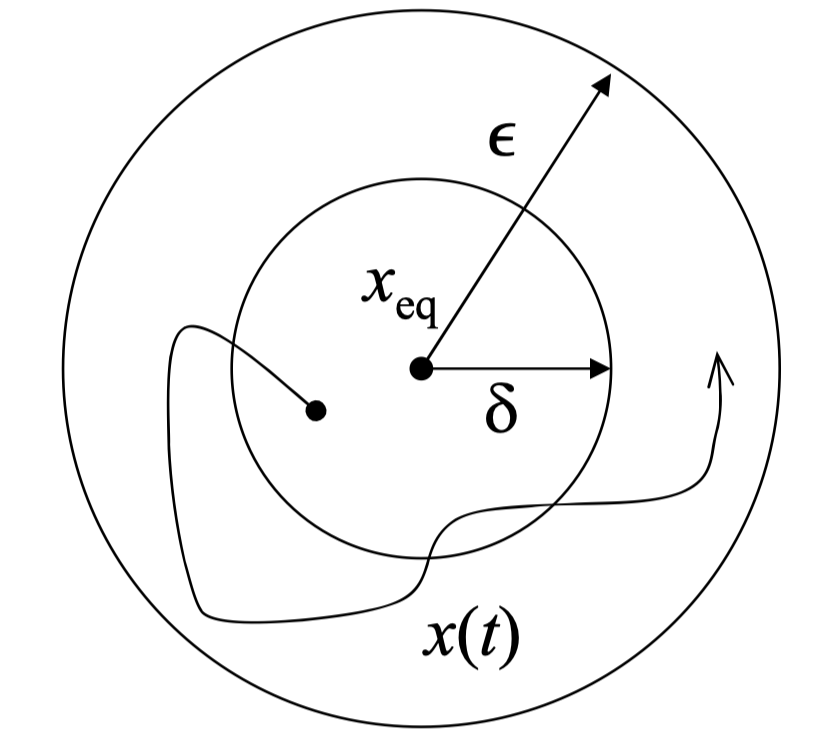
\includegraphics[width=0.4\textwidth]{Figs/1.png}
    \caption{$\epsilon-\delta$ definition of stability.}
    \label{fig:stabepsilon_delta}
\end{figure}
\subsubsection{Continuity Definition}
\begin{defa}We first list several concepts:
\begin{itemize}
    \item $\mathcal{X}_{\text {sig }} \equiv$ set of all piecewise continuous signals taking values in $\mathbb{R}^{n}$
    \item Signal norm: Given a signal $x \in \mathcal{X}_{\mathrm{sig}},\|x\|_{\mathrm{sig}}:=\sup _{t \geq 0}\|x(t)\|$
    \item ODE can be seen as an operator
$\mathrm{T}: \mathbb{R}^{n} \rightarrow \mathcal{X}_{\mathrm{sig}}$ that maps $x_{0} \in \mathbb{R}^{n}$ into the solution that starts at $x(0)=x_{0}$
\end{itemize}
The equilibrium point $x_{\mathrm{eq}} \in \mathbb{R}^{n}$ is \tb{(Lyapunov) stable} if $\mathrm{T}$ is continuous at $x_{\mathrm{eq}}$ :
\begin{align*}
\forall \epsilon>0, \exists \delta>0:\left\|x_{0}-x_{\mathrm{eq}}\right\| \leq \delta \Longrightarrow \underbrace{\left\|\mathrm{T}\left(x_{0}\right)-\mathrm{T}\left(x_{\mathrm{eq}}\right)\right\|_{\mathrm{sig}} \leq \epsilon}_{\sup _{t \geq 0}\left\|x(t)-x_{\mathrm{eq}}\right\| \leq \epsilon}
\end{align*}
\end{defa}
\begin{rema}\bfs{stability of arbitrary solutions}
It can be extended to \tb{nonequilibrium solutions} as shown below in \cref{fig:stabanysolution} and defined below:

A solution $x^{*}$ is \tb{(Lyapunov) stable} if $\mathrm{T}$ is continuous at $x^{*}{ }_{0}:=x^{*}(0)$, i.e.,
\begin{align*}
\forall \epsilon>0, \exists \delta>0:\left\|x_{0}-x^{*}{ }_{0}\right\| \leq \delta \Longrightarrow \underbrace{\left\|\mathrm{T}\left(x_{0}\right)-\mathrm{T}\left(x_{0}^{*}\right)\right\|_{\operatorname{sig}} \leq \epsilon}_{\sup _{t \geq 0}\left\|x(t)-x^{*}(t)\right\| \leq \epsilon}
\end{align*}
\end{rema}
\begin{figure}[H]
    \centering
    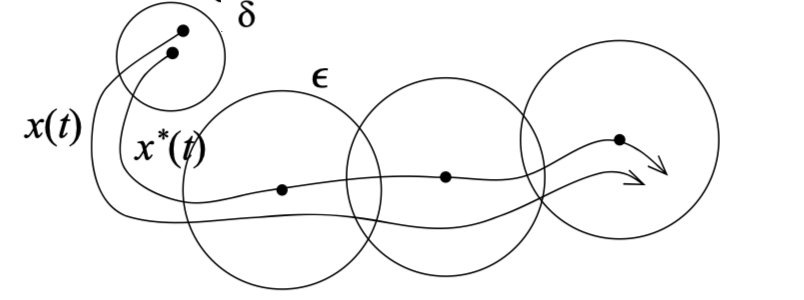
\includegraphics[width=0.6\textwidth]{Figs/2.png}
    \caption{$\epsilon-\delta$ definition of stability.}
    \label{fig:stabanysolution}
\end{figure}
\subsubsection{Class $\mathcal{K}$ Function Definition}
We first give the definition of class $\mathcal{K}$ function.
\begin{defa}\bfs{Class $\mathcal{K}$ Function}
Class $\mathcal{K} \equiv \operatorname{set}$ of functions $\alpha:[0, \infty) \rightarrow[0, \infty)$ that are
\begin{enumerate}
    \item continuous
    \item strictly increasing
    \item $\alpha(0)=0$
\end{enumerate}
\end{defa}
\begin{defa}\label{def:kstable}
The equilibrium point $x_{\mathrm{eq}} \in \mathbb{R}^{n}$ is \tb{(Lyapunov) stable} if $$\exists \alpha \in \mathcal{K},
\left\|x(t)-x_{\mathrm{eq}}\right\| \leq \alpha\left(\left\|x\left(t_{0}\right)-x_{\mathrm{eq}}\right\|\right), \forall t \geq t_{0} \geq 0\text{ and } \left\|x\left(t_{0}\right)-x_{\mathrm{eq}}\right\| \leq \mathrm{c}$$
\end{defa}
\begin{rema}\bfs{some explanation}
\begin{enumerate}
    \item Strictly increasing is because if $c_1<c_2$, we have $\alpha(c_1)<\alpha(c_2)$ to show the region of $x(t)$ should be strictly smaller with starting points $x_0$ which has smaller distance from $x_{\mathrm{eq}}$. Think in a subset way. 
    \item Continuous is because ode is about integration and $x$ is continuous? (Not sure. Need to look back again). Why $\alpha$ cannot be piece wise continuous with some discontinuous points? It seems intuitive and reasonable but need some proof.
    \item $\alpha(0)=0$ is for equilibrium. 
    \item The function $\alpha$ can be constructed directly from the $\delta(\epsilon)$ in the $\epsilon-\delta$ (or continuity) definitions.
\end{enumerate}
\end{rema}

\begin{figure}[H]
     \centering
     \begin{subfigure}[b]{0.3\textwidth}
         \centering
         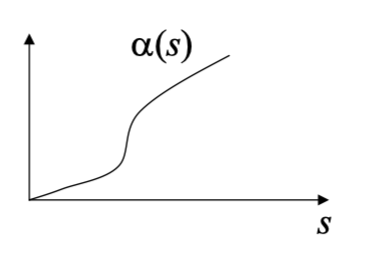
\includegraphics[width=\textwidth]{Figs/3.png}
         \caption{function $\alpha$}
     \end{subfigure}
     \hfill
     \begin{subfigure}[b]{0.47\textwidth}
         \centering
         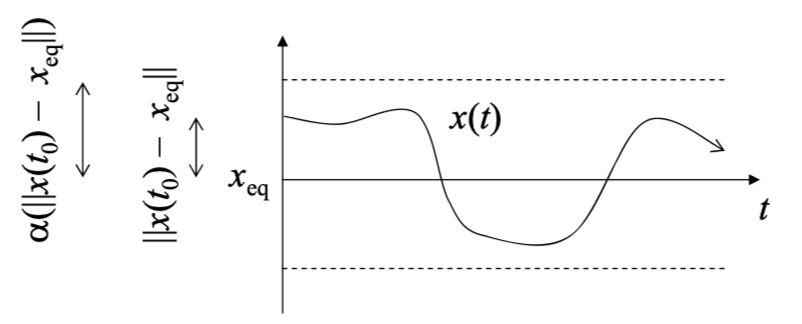
\includegraphics[width=\textwidth]{Figs/4.png}
     \end{subfigure}
\end{figure}

\subsection{Asymptotic Stability}
Asymptotic stability is stronger than stability since we need it to converge to $0$ when $t\rightarrow \infty$. For simplicity,
here we care about the globally asymptotically stable instead of the local one.
\subsubsection{Convergence Definition}
\begin{figure}[H]
    \centering
    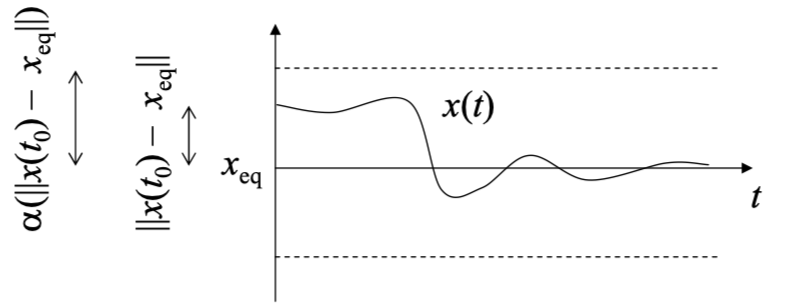
\includegraphics[width=0.6\textwidth]{Figs/7.png}
    \caption{asymptotically stable.}
\end{figure}
\begin{defa}
The equilibrium point $x_{\mathrm{eq}} \in \mathbb{R}^{n}$ is (globally) asymptotically stable if it is Lyapunov stable and for every initial state the solution exists on $[0, \infty)$ and $$x(t) \rightarrow x_{e}\text{ as }t \rightarrow \infty.$$
\end{defa}

\subsubsection{Class $\mathcal{KL}$ Function Definition}
\begin{defa}\bfs{Class $\mathcal{KL}$ Function}
Class  $\mathcal{K}L \equiv$ set of functions $\beta:[0, \infty) \times[0, \infty) \rightarrow[0, \infty)$ s.t.
\begin{enumerate}
    \item For each fixed  $t$, $\beta(\cdot, t) \in \mathcal{K}$,
    \item For each fixed $s$, $\beta(s, \cdot)$ is monotone decreasing and $\beta(s, t) \rightarrow 0 \text { as } t \rightarrow \infty$
\end{enumerate}
\end{defa}
\begin{figure}[H]
     \centering
     \begin{subfigure}[b]{0.4\textwidth}
         \centering
         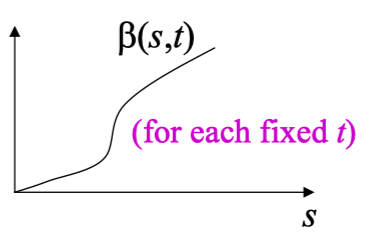
\includegraphics[width=\textwidth]{Figs/5.png}
         \caption{function $\beta$ with fixed $t$}
     \end{subfigure}
     \hfill
     \begin{subfigure}[b]{0.4\textwidth}
         \centering
         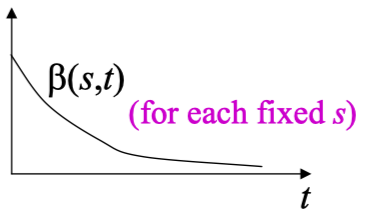
\includegraphics[width=\textwidth]{Figs/6.png}
         \caption{function $\beta$ with fixed $s$}
     \end{subfigure}
\end{figure}
\begin{defa}
 The equilibrium point $x_{\mathrm {eq}} \in \mathbb{R}^{n}$ is \tb{(globally) asymptotically stable} if $\exists \beta \in \mathcal{K} \mathcal{L}$:
$$\|x(t)-x\|<\beta(\|x(t)-x\|, t-t_0), \forall t\ge t_0\ge0$$
\end{defa}
\begin{rema}\bfs{exponential stability}
We have exponential stability when
$\beta(s, t)=c e^{-\lambda t} s$ with $c, \lambda>0$. It is linear in $s$ and negative exponential in $t$.
\end{rema}


\begin{figure}[H]
    \centering
    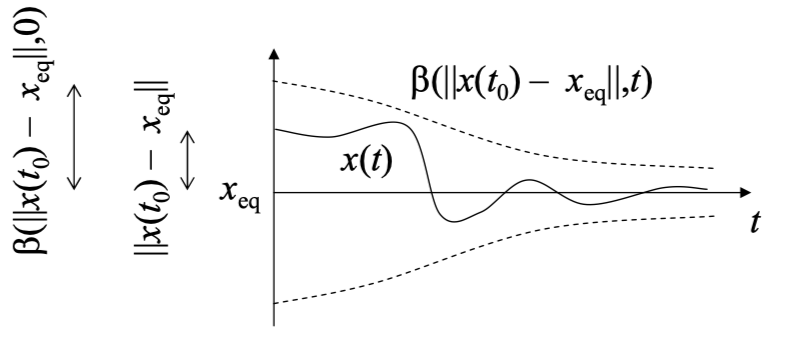
\includegraphics[width=0.6\textwidth]{Figs/8.png}
    \caption{asymptotically stable using $\mathcal{KL}$ function class.}
\end{figure}


\subsection{Lyapunov’s Stability Theorem}
Suppose we could show that $\left\|x(t)-x_{\mathrm{eq}}\right\|$ always decreases along solutions to the ODE. Then
$\left\|x(t)-x_{\mathrm{eq}}\right\| \leq\left\|x\left(t_{0}\right)-x_{\mathrm{eq}}\right\|\quad \forall t \geq t_{0} \geq 0$, i.e.
we could pick $\alpha(s)=s \Rightarrow$ Lyapunov stability. We can draw the same conclusion by using other measures of how far the solution is from $x_{\mathrm {eq}}$.

$\bullet$ \tb{Lyapunov Function Is a Distance Measure}
\begin{defa}\bfs{Positive Definite $V$}
 $V: \mathbb{R}^{n} \rightarrow \mathbb{R}$ \tb{positive definite}, i.e. $V(x) \geq 0,  \forall x \in \mathbb{R}^{n}$ with $=0$ only for $x=0$:
\begin{align*}
V\left(x-x_{\mathrm{eq}}\right) \quad \begin{cases}=0 & x=x_{\mathrm{eq}} \\ >0 & x \neq x_{\mathrm{eq}}\end{cases}
\end{align*}
\end{defa}
\begin{rema}
It provides a measure of how far $x$ is from $x_{\mathrm {eq}}$ (not necessarily a metric-may not satisfy triangular inequality). Note $V$ is not only \tb{positive semi-definite} (avoid $V(x)=0$ for some $x\ne 0$).
\end{rema}
\begin{defa}\bfs{Radially Unbounded $V$}
We call $V: \mathbb{R}^{n} \rightarrow \mathbb{R}$ is radially unbounded, if additionally $x \rightarrow \infty \Rightarrow V(x) \rightarrow \infty$:
\begin{align*}
V\left(x-x_{\mathrm{eq}}\right) \quad \begin{cases}=0 & x=x_{\mathrm{eq}} \\ >0 & x \neq x_{\mathrm{eq}} \\ \rightarrow \infty & \left\|x-x_{\mathrm{eq}}\right\| \rightarrow \infty\end{cases}
\end{align*}
\end{defa}
\begin{rema}\bfs{explanation and gradient of $V$}

Q: How to check if $V\left(x(t)-x_{e q}\right)$ decreases along solutions?
\begin{align*}
\begin{aligned}
\frac{\mathrm{d}}{\mathrm{d} t} V\left(x(t)-x_{\mathrm{eq}}\right) &=\frac{\partial V}{\partial x}\left(x(t)-x_{\mathrm{eq}}\right) \dot{x}(t) \\
&=\frac{\partial V}{\partial x}\left(x(t)-x_{\mathrm{eq}}\right) f(x(t))
\end{aligned}
\end{align*}
$A: V\left(x(t)-x_{e q}\right)$ will decrease if  gradient of $V$
\begin{align*}
\frac{\partial V}{\partial x}\left(z-x_{\mathrm{eq}}\right) f(z) \leq 0 \quad \forall z \in \mathbb{R}^{n}
\end{align*}
Note  here it can be computed without actually computing the solution $x(t)$ of the ODE.
\end{rema}

\begin{figure}[H]
    \centering
    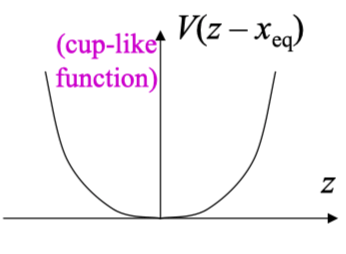
\includegraphics[width=0.4\textwidth]{Figs/9.png}
    \caption{cup-like function $V$.}
    \label{fig:V}
\end{figure}
\begin{thma}\bfs{Lyapunov Stable Theorem I}
Suppose there exists a continuously differentiable, positive definite function $V$ : $\mathbb{R}^{n} \rightarrow \mathbb{R}$ such that
\begin{align*}
\frac{\partial V}{\partial x}\left(z-x_{\mathrm{eq}}\right) f(z) \leq 0 \quad \forall z \in \mathbb{R}^{n}
\end{align*}
Then $x_{\mathrm{eq}}$ is a \tb{Lyapunov stable equilibrium.}
\end{thma}
\begin{proof}
$V$ non increasing $\Rightarrow V\left(x(t)-x_{\mathrm{eq}}\right) \leq V\left(x\left(t_{0}\right)-x_{\mathrm{eq}}\right) \forall t \geq t_{0}$
Thus, by making $x\left(t_{0}\right)-x_{\mathrm{eq}}$ small we can make $V\left(x(t)-x_{\mathrm{eq}}\right)$ arbitrarily small $\forall t \geq t_{0}$ So, by making $x\left(t_{0}\right)-x_{\mathrm{eq}}$ small we can make $x(t)-x_{\mathrm{eq}}$ arbitrarily small $\forall t \geq t_{0}$. We can actually compute $\alpha$ from $V$ explicitly and take $c=+\infty$ using \cref{def:kstable}.
\end{proof}

\begin{thma}\bfs{Lyapunov Stable Theorem II}
Suppose there exists a continuously differentiable, positive definite, \tb{radially unbounded function} $V: \mathbb{R}^{n} \rightarrow \mathbb{R}$ such that
\begin{align*}
\frac{\partial V}{\partial x}\left(z-x_{\mathrm{eq}}\right) f(z) \leq 0 \quad \forall z \in \mathbb{R}^{n}
\end{align*}
Then $x_{\mathrm {eq}}$ is a Lyapunov stable equilibrium and \tb{the solution always exists globally}. Moreover, if $=0$ only for $z=x_{\mathrm{eq}}$ then $x_{\mathrm{eq}}$ is a globally \tb{asymptotically stable equilibrium.}
\end{thma}
\begin{proof}
$V$ can only stop decreasing when $x(t)$ reaches $x_{\mathrm {eq}}$, but $V$ must stop decreasing because it cannot become negative Thus, $x(t)$ must converge to $x_{\mathrm{eq}}$. See ``Laypunov stable\_2.pdf'' for details, where we also need to use compactness from radially unboundness to prove global stable.
\end{proof}
\begin{thma}\bfs{Lyapunov Stable Theorem: A Summary}
\begin{enumerate}
    \item The equilibrium point is stable if there is a continuously differentiable positive definite function $V(x)$ so that $\dot{V}(x)$ is negative semidefinite (i.e. $\dot{V}(x)\le 0$).
    \item It is (not necessarily globally) asymptotically stable if $\dot{V}(x)$ is negative definite (i.e. $\dot{V}(x)=0$ only if $x=0$).
    \item It is globally asymptotically stable if the conditions for asymptotic stability hold globally and $V(x)$ is radially unbounded.
\end{enumerate}
\end{thma}
\begin{proof}
See supp Laypunov stable\_2.pdf where the compact and continuous of $V$ is used.
\end{proof}
\subsection{LaSalle’s Invariance Principle}
What if
\begin{align*}
\frac{\partial V}{\partial x}\left(z-x_{\mathrm {eq}}\right) f(z)=0 \quad \forall z \in \mathbb{R}^{n}
\end{align*}
for other $z$ than $x_{e q}$ ? Can we still claim some form of convergence?
\begin{defa}\bfs{Invariant Set}
We still consider \cref{eq:ode}: $\dot{x}=f(x) \quad x \in \mathbb{R}^{n}$.  We call
$M \in \mathbb{R}^{n}$ is an \tb{invariant set} $\equiv x\left(t_{0}\right) \in M \Rightarrow x(t) \in M, \forall t \geq t_{0}$
%(in the context of hybrid systems: $\operatorname{Reach}(M) \subset M \ldots$ )
\end{defa}
\begin{thma}\bfs{LaSalle Invariance Principle}
Suppose there exists a continuously differentiable, positive definite, \tb{radially unbounded} function $V: \mathbb{R}^{n} \rightarrow \mathbb{R}$ such that
\begin{align*}
\frac{\partial V}{\partial x}\left(z-x_{\mathrm {eq}}\right) f(z) \leq W(z) \leq 0 \quad \forall z \in \mathbb{R}^{n}
\end{align*}
Then $x_{\mathrm{eq}}$ is a Lyapunov stable equilibrium and the solution always exists globally. Moreover, $x(t)$ converges to the largest invariant set $M$ contained in
\begin{align*}
E:=\left\{z \in \mathbb{R}^{\mathrm{n}}: W(z)=0\right\}
\end{align*}
\end{thma}
\begin{rema}\bfs{compare to Lyapunov Theorem}
Note that:
\begin{enumerate}
    \item When $W(z)=0$ only for $z=x_{\mathrm{eq}}$ then $E=\left\{x_{\mathrm{eq}}\right\}$.
Since $M \subset E, M=\left\{x_{\mathrm{eq}}\right\}$ and therefore $x(t) \rightarrow x_{e q} \Rightarrow$ asympt. stability. That means Lyapunov Theorem is a speical case LaSalle Invariance Principle.
\item Even when $E$ is larger then $\left\{x_{\mathrm{eq}}\right\}$ we often have $M=\left\{x_{\mathrm{eq}}\right\}$ and can conclude asymptotic stability.
\end{enumerate} 
\end{rema}
\subsection{Linear systems}
Consider the following linear ODE:
\begin{align*}
\dot{x}=A x \quad x \in \mathbb{R}^{n}, A \in \mathbb{R}^{n \times n}
\end{align*}
We have the solution:
\begin{align*}
x(t)=e^{A\left(t-t_{0}\right)} x\left(t_{0}\right) \quad t \geq t_{0} \quad e^{A \tau}:=\sum_{k=0}^{\infty} \frac{\tau^{k}}{k !} A^{k}
\end{align*}
\begin{thma}
The origin $x_{\mathrm{eq}}=0$ is an equilibrium point. It is
\begin{itemize}
    \item \tb{Lyapunov stable} if and only if all eigenvalues of $A$ have negative or zero real parts and for each eigenvalue with zero real part there is an independent eigenvector.
    \item \tb{Asymptotically stable} if and only if all eigenvalues of $A$ have negative real parts. In this case the origin is actually exponentially stable
\end{itemize} 
\end{thma}
\begin{thma}
The origin $x_{\mathrm{eq}}=0$ is an equilibrium point. It is asymptotically stable if and only if for every positive symmetric definite matrix $Q$ the \tb{Lyapunov equation}
$$A^{\prime} P+P A=-Q$$
has a unique solutions $P$ that is symmetric and positive definite.
\end{thma}
\begin{proof}
We have 
\begin{figure}[H]
     \centering
     \begin{subfigure}[b]{0.8\textwidth}
         \centering
         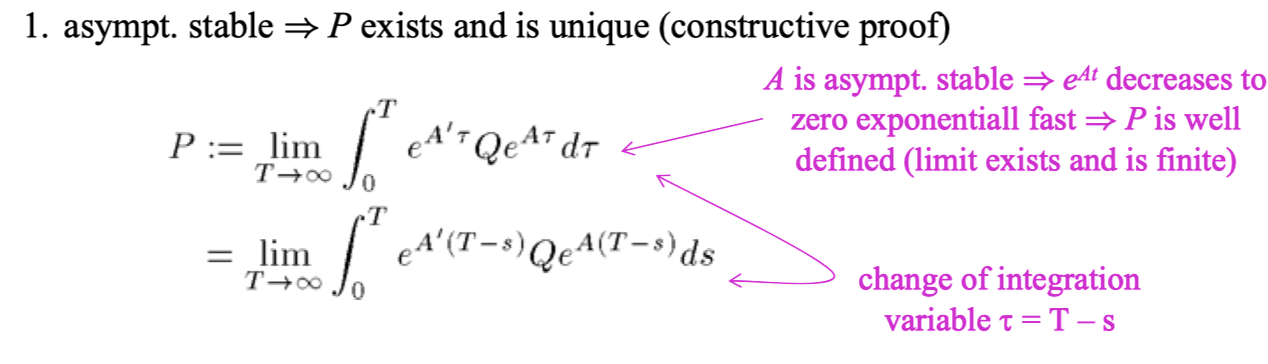
\includegraphics[width=\textwidth]{Figs/10.png}
     \end{subfigure}
     \vfill
     \begin{subfigure}[b]{0.8\textwidth}
         \centering
         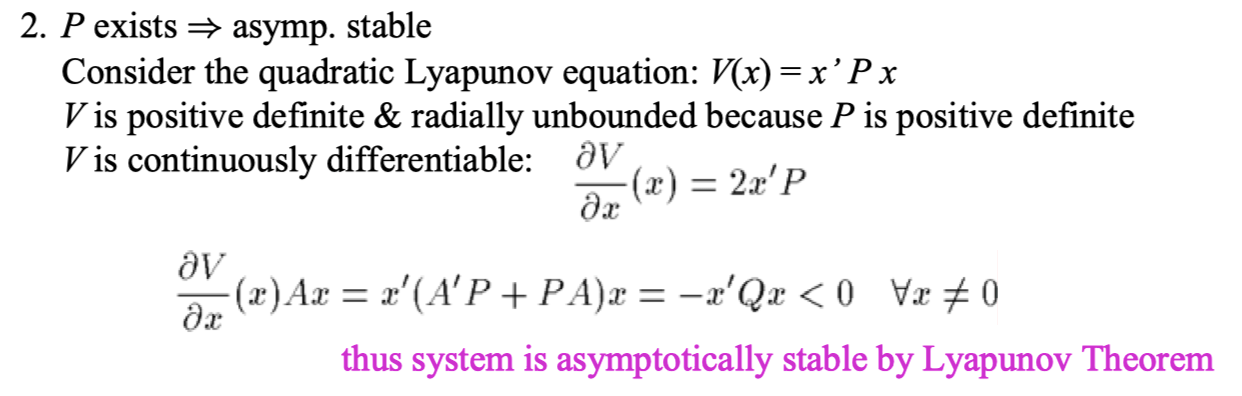
\includegraphics[width=\textwidth]{Figs/11.png}
     \end{subfigure}
\end{figure}
\end{proof}

\section{Basic Theorem}
\subsection{Basic Thorems from Real Analysis}
\subsubsection{Basic Concepts}
"Function" below generally means a map from some specified set of a vector space $\mathbf{R}^{e}$ into a space $\mathbf{R}^{d}$, not always of the same dimension. $\mathbf{R}^{d}$ denotes a normed, real $d$-dimensional vector space of elements $y=$ $\left(y^{1}, \ldots, y^{d}\right)$ with norm $|y|$. Unless otherwise specified, $|y|$ will be the norm
\begin{align*}
|y|=\max \left(\left|y^{1}\right|, \ldots,\left|y^{d}\right|\right)
\end{align*}
and $\|y\|$ the Euclidean norm.


If $y_{0}$ is a point and $E$ a subset of $\mathbf{R}^{d}$, then dist $\left(y_{0}, E\right)$, the distance from $y_{0}$ to $E$, is defined to be inf $\left|y_{0}-y\right|$ for $y \in E$. If $E_{1}, E_{2}$ are two subsets of $\mathbf{R}^{d}$, then dist $\left(E_{1}, E_{2}\right)$ is defined to be inf $\left|y_{1}-y_{2}\right|$ for $y_{1} \in E_{1}, y_{2} \in E_{2}$, and is called the distance between $E_{1}$ and $E_{2}$. If $E_{1}$ (or $E_{2}$ ) is compact and $E_{1}, E_{2}$ are closed and disjoint, then dist $\left(E_{1}, E_{2}\right)>0$.

If $E$ is an open set or a closed parallelepiped in $\mathbf{R}^{d}, f \in C^{n}(E), 0 \le n<$ $\infty$, means that $f(y)$ is continuous on $E$ and that the components of $f$ have continuous partial derivatives of all orders $k \le n$ with respect to $y^{1}, \ldots, y^{d} .$
A function $f(y, z)=f\left(y^{1}, \ldots, y^{d}, z^{1}, \ldots, z^{e}\right)$ defined on a $(y, z)$-set $E$, where $y \in \mathbf{R}^{d}$, is said to be uniformly Lipschitz continuous on $E$ with respect to $y$ if there exists a constant $K$ satisfying
\begin{align*}
\left|f\left(y_{1}, z\right)-f\left(y_{2}, z\right)\right| \le K\left|y_{1}-y_{2}\right| \quad \text { for all } \quad\left(y_{j}, z\right) \in E
\end{align*}
with $j=1,2 .$ Any constant $K$ satisfying $\cref{eq:kdad}$ is called a Lipschitz constant (for $f$ on $E$ ). (The admissible values of $K$ depend, of course, on the norms in the $f$ - and $y$-spaces.)

A family $F$ of functions $f(y)$ defined on some $y$-set $E \subset \mathbf{R}^{d}$ is said to be equicontinuous if, for every $\epsilon>0$, there exists a $\delta=\delta_{\epsilon}>0$ such that $\left|f\left(y_{1}\right)-f\left(y_{2}\right)\right| \le \epsilon$ whenever $y_{1}, y_{2} \in E,\left|y_{1}-y_{2}\right| \le \delta$ and $f \in F$. The point of this definition is that $\delta_{\epsilon}$ does not depend on $f$ but is admissible for all $f \in F$. The most frequently encountered equicontinuous families $F$ below will occur when all $f \in F$ are uniformly Lipschitz continuous on $E$ and there exists a $K>0$ which is a Lipschitz constant for all $f \in F$; in which case, $\delta$ can be chosen to be $\delta=\epsilon / K$.

\begin{lema}\label{lem:efda}
If a sequence of continuous functions on a compact set $E$ is uniformly convergent on $E$, then it is uniformly bounded and equicontinuous.
\end{lema}
\subsubsection{Cantor Selection}
\begin{thma}\bfs{Cantor Selection}
Let $f_{1}(y), f_{2}(y), \ldots$ be a uniformly bounded sequence of functions on a $y$-set $E$. Then for any countable set $D \subset E$, there exists a subsequence $f_{n(1)}(y), f_{n(2)}(y), \ldots$ convergent on $D .$
\end{thma} 

\subsubsection{Ascoli}
\begin{thma}\bfs{Ascoli}\label{thm:Ascoli}
On a compact $y$-set $E$, let $f_{1}(y), f_{2}(y), \ldots$ be a sequence of functions which is equicontinuous and convergent on a dense subset of $E$. Then $f_{1}(y), f_{2}(y), \ldots$ converges uniformly on $E$.
\end{thma}
\subsubsection{Arzela}
\begin{thma}\bfs{Arzela}\label{thm:Arzela} On a compact $y$-set $E \subset \mathbf{R}^{d}$, let $f_{1}(y), f_{2}(y), \ldots$ be a sequence of functions which is pointwise bounded and equicontinuous.
\begin{enumerate}
\item They are uniformly bounded.
    \item Then there exists a subsequence $f_{n(1)}(y), f_{n(2)}(y), \ldots$ which is uniformly convergent on $E$.
\end{enumerate}
\end{thma}

The follwing remarks are also import:
\begin{rema}
If, in \cref{thm:Arzela} $y_{0} \in E$ and $f_{0}$ is a limit point of the sequence $f_{1}\left(y_{0}\right), f_{2}\left(y_{0}\right), \ldots$, then the subsequence $f_{n(1)}(y), f_{n(2)}(y), \ldots$ in the assertion can be chosen so that the limit function $f(y)$ satisfies $f\left(y_{0}\right)=f_{0}$.
\end{rema}
\begin{rema}\label{re:mdiohqefr}
If, in \cref{thm:Arzela}, it is known that all (uniformly) convergent subsequences of $f_{1}(y), f_{2}(y), \ldots$ have the same limit, say $f(y)$, then a selection is unnecessary and $f(y)$ is the uniform limit of $f_{1}(y), f_{2}(y), \ldots$.
\end{rema} 

\subsubsection{Convergence of ODE I}
\begin{thma}\label{thm:conv_ode}
Let $y, f \in \mathbf{R}^{d}$ and $f_{0}(t, y), f_{1}(t, y), f_{2}(t, y), \ldots$ be a sequence of continuous functions on the parallelepiped $R: t_{0} \le t \le t_{0}+a, \mid y-$ $y_{0} \mid \le b$ such that
\begin{align}
    f_{0}(t, y)=\lim _{n \rightarrow \infty} f_{n}(t, y)\text{ uniformly on }R. \label{eq:jdad}
\end{align}
Let $y_{n}(t)$ be a solution of
\begin{align}
    y^{\prime}=f_{n}(t, y), \quad y\left(t_{n}\right)=y_{n}\label{eq:rfasd}
\end{align}
on $\left[t_{0}, t_{0}+a\right]$, where $n=1,2, \ldots$, and
\begin{align}
    t_{n} \rightarrow t_{0}, y_{n} \rightarrow y_{0} \quad\text{ as }\quad n \rightarrow \infty
\end{align}
Then 
\begin{enumerate}[1)]
    \item there exists a subsequence $y_{n(1)}(t), y_{n(2)}(t), \ldots$ which is \tb{uniformly convergent} on $\left[t_{0}, t_{0}+a\right]$. \item For any such subsequence, the limit
\begin{align}
y_{0}(t)=\lim _{k \rightarrow \infty} y_{n(k)}(t)\label{eq:dagz}
\end{align}
is a solution of \cref{eq:rfasd} with $n=0$ on $\left[t_{0}, t_{0}+a\right]$. 
\item In particular, if \cref{eq:rfasd} with $n=0$  possesses $a$ unique solution $y=y_{0}(t)$ on $\left[t_{0}, t_{0}+a\right]$, then
\begin{align}
y_{0}(t)=\lim _{n \rightarrow \infty} y_{n}(t) \quad \text { uniformly on }\left[t_{0}, t_{0}+a\right] .\label{eq:odadf}
\end{align}
\end{enumerate}
\end{thma} 
\begin{proof}
\tb{proof of 1).:} Since $f_{1}, f_{2}, \ldots$ are continuous and \cref{eq:jdad} holds uniformly on $R$, there is a constant $K$ such that $\left|f_{n}(t, y)\right| \le K$ for $n=0,1, \ldots$ and $(t, y) \in R$. Since $\left|y_{n}^{\prime}(t)\right| \le K$, from \cite[Theorem 5.19]{rudin1976principles} it is clear that $K$ is a Lipschitz constant for \tb{all} $y_{1}, y_{2}, \ldots$. We therefore have the sequence $y_{1}, y_{2}, \ldots$ is equicontinuous. It is also uniformly bounded since $\left|y_{n}(t)-y_{0}\right| \le b$. Thus the existence of uniformly convergent subsequences follows from \cref{thm:Arzela}. 

\tb{proof of 2).:} By \cref{eq:jdad}, \cref{lem:efda}, and the uniformity of \cref{eq:dagz}, it is easy to see that
\begin{align*}
f_{n(k)}\left(t, y_{n(k)}(t)\right) \rightarrow f_{0}\left(t, y_{0}(t)\right)
\end{align*}
uniformly on $\left[t_{0}, t_{0}+a\right]$ as $k \rightarrow \infty$. Thus term-by-term integration is applicable to
\begin{align*}
y_{n}(t)=y_{n}+\int_{t_{n}}^{t} f_{n}\left(s, y_{n}(s)\right) d s
\end{align*}
where $n=n(k)$ and $k \rightarrow \infty$. It follows that the limit \cref{eq:dagz} is a solution of \cref{eq:rfasd} with $n=0$ .

\tb{proof of 3).:} Note that the assumed uniqueness of the solution $y_{0}(t)$ of \cref{eq:rfasd} with $n=0$  shows that the limit of every (uniformly) convergent subsequence of $y_{1}(t), y_{2}(t), \ldots$ is the solution $y_{0}(t)$. Hence a selection is unnecessary and \cref{eq:odadf} holds by \cref{re:mdiohqefr}.
\end{proof} 

\subsubsection{Implicit Function }
\begin{thma}\bfs{Implicit Function}
Let $x, y, f, g$ be d-dimensional vectors and $z$ an e-dimensional vector. Let $f(y, z)$ be continuous for $(y, z)$ near a point $\left(y_{0}, z_{0}\right)$ and have continuous partial derivatives with respect to the components of $y .$ Let the Jacobian $\operatorname{det}\left(\partial f^{j} / \partial y^{k}\right) \neq 0$ at $(y, z)=\left(y_{0}, z_{0}\right)$. Let $x_{0}=f\left(y_{0}, z_{0}\right)$. Then there exist positive numbers, $\epsilon$ and $\delta$, such that if $x$ and $z$ are fixed, $\left|x-x_{0}\right|<\delta$ and $\left|z-z_{0}\right|<\delta$, then the equation $x=$ $f(y, z)$ has a unique solution $y=g(x, z)$ satisfying $\left|y-y_{0}\right|<\epsilon$. Furthermore, $g(x, z)$ is continuous. for $\left|x-x_{0}\right|<\delta,\left|z-z_{0}\right|<\delta$ and has continuous partial derivatives with respect to the components of $x$.
\end{thma}
 
 \subsubsection{Smooth Approximations}\label{sec:smooth_app}
In some situations, it will be convenient to extend the definition of a function $f$, say, given continuous on a closed parallelepiped, or to approximate it uniformly by functions which are smooth $\left(C^{1}\right.$ or $\left.C^{\infty}\right)$ with respect to certain variables. The following approach can be used to obtain such extensions or approximations (which have the same bounds as $f$).

Let $f(t, y)$ be defined on $R: t_{0} \le t \le t_{1},|y| \le b$ and let $|f(t, y)| \le M$.

$\bullet$ \tb{Extension:}

\tb{Case I:} We can extend $f$ to a continuous $f^*$ as: 
\begin{enumerate}
    \item Let $f^{*}(t, y)$ be defined for $t_{0} \le t \le t_{1}$ and all $y$ by placing $f^{*}(t, y)=f(t, y)$ if $|y| \le b$.
    \item Let $f^{*}(t, y)=f(t, b y/ |y|)$ if $|y|>b$.
\end{enumerate} It is clear that $f^{*}(t, y)$ is continuous for $t_{0} \le t \le t_{1}, y$ arbitrary, and that $\left|f^{*}(t, y)\right| \le M .$ 

\tb{Case II:} In some cases, we need a $f^{*}$ by an extension of $f$ which is \tb{$0$ for large $|y|$}:
\begin{enumerate}
    \item  Let $f^{*}(t, y)$ be defined as above.
    \item Let $f^{0}(t, y)=f^{*}(t, y) \varphi^{0}(|y|)$, where $\varphi^{0}(s)$ is a continuous function for $t \ge 0$ satisfying $0 \le \varphi^{0}(s) \le 1$ for $s \ge 0$: 
    \begin{enumerate}
        \item $\varphi^{0}(s)=1$ for $0 \le s \le b$
        \item $\varphi^{0}(s)=0$ for $s \ge b+1 .$
    \end{enumerate}
\end{enumerate}

$\bullet$ \tb{Uniformly $C^\infty$ Approximate:}

Similar to \cite[P139 Lemma 4.1.1]{mtnotes}. In order to approximate $f(t, y)$ uniformly on $R$ by functions $f^{\epsilon}(t, y)$ which are, say, smooth with respect to the components of $y$, let $\varphi(s)$ be \tb{a function of class $C^{\infty}$} for $s \ge 0$ satisfying
\begin{enumerate}
    \item  $\varphi(s)>0$ for $0 \le s<1$ and
    \item $\varphi(s)=0$ for $s \ge 1$.
\end{enumerate}Then there is a constant $c>0$ (we can also cooperate it to $\varphi$) depending only on $\varphi(s)$ and the dimension $d$, such that for every $\epsilon>0$,
\begin{align}
c \epsilon^{-d} \int_{-\infty}^{+\infty} \cdots \int_{-\infty}^{+\infty} \varphi\left(\epsilon^{-2}\|y\|^{2}\right) d y^{1} \ldots d y^{d}=1\label{eq:3.1I}
\end{align}
where $\|y\|=\left(\Sigma\left|y^{k}\right|^{2}\right)^{1 / 2}$ is the Euclidean length of $y$. Put
\begin{align}
    f^{\epsilon}(t, y)=c \epsilon^{-d} \int_{-\infty}^{+\infty} \cdots \int_{-\infty}^{+\infty} f^{0}(t, \eta) \varphi\left(\epsilon^{-2}\|y-\eta\|^{2}\right) d \eta^{1} \ldots d \eta^{d}\label{eq:3.2I}
\end{align}
where $\eta=\left(\eta^{1}, \ldots, \eta^{d}\right)$, which is equivalent to 
\begin{align}
    f^{\epsilon}(t, y)=c \epsilon^{-d} \int_{-\infty}^{+\infty} \ldots \int_{-\infty}^{+\infty} f^{0}(t, y-\eta) \varphi\left(\epsilon^{-2}\|\eta\|^{2}\right) d \eta^{1} \ldots d \eta^{d}.\label{eq:3.3I}
\end{align}
Since $f^{\epsilon}(t, y)$ is an "average" of the values of $f^{0}$ in a sphere $\|\eta-y\| \le \epsilon$ for a fixed $t$, it is intuitively true that $f^{t} \rightarrow f^{0}$ as $\epsilon \rightarrow 0$ uniformly on $t_{0} \le t \le t_{1}, y$ arbitrary.  \tb{Lebesgue Dominated Convergent Theorem} can be used to prove $f^\epsilon\in C^\infty$ w.r.t. $y$ and uniformly convergence follows from the continuous of $f^0$ and the compact support of $\phi$. We have $\left|f^{\epsilon}\right| \le M$ for all $\epsilon>0$ and that $f^{*}(t, y)=0$ for $|y| \geq b+1+\epsilon$.





\subsection{The Picard-Lindel\"of Theorem}
Various types of existence proofs will be given. One of the most simple and useful is the following.
\begin{thma}\label{thm:djhfads}
Let $y, f \in \mathbf{R}^{d} ; f(t, y)$ continuous on a parallelepiped $R: t_{0} \le t \le t_{0}+a,\left|y-y_{0}\right| \le b$ and \tb{uniformly Lipschitz continuous} with respect to $y$. Let $M$ be a bound for $|f(t, y)|$ on $R$; $\alpha=\min (a, b / M)$. Then
\begin{align}
    y^{\prime}=f(t, y), \quad y\left(t_{0}\right)=y_{0}\label{eq:jdfeq}
\end{align}
has a \tb{unique} solution $y=y(t)$ on $\left[t_{0}, t_{0}+\alpha\right]$.
\end{thma}
\subsection{Peano's Existence Theorem}
The next theorem to be proved drops the assumption of Lipschitz continuity and the assertion of uniqueness.
\begin{thma} \label{thm:Peano}We have the following conditions:
\begin{enumerate}
    \item  Let $y, f \in \Real^{d} ; f(t, y)$ continuous on set $$R=\{ t_{0} \le t \le t_{0}+a, \left|y-y_{0}\right| \le b \}.$$ 
    \item We also have that $M$ is a bound for $|f(t, y)|$ on $R$.
\end{enumerate}

  Let $\alpha=\min (a, b / M)$. 
 We then  have the following conclusion:
 \begin{itemize}
     \item \cref{eq:jdfeq} possesses \tb{at least one solution} $y=y(t)$ on $\left[t_{0}, t_{0}+\alpha\right]$.
 \end{itemize}
 
\end{thma}
\begin{rema}
In this theorem, $|y|$ can be any convenient norm on $\mathbf{R}^{d}$.
\end{rema}
An important consequence of Peano's existence theorem will often be used:

\begin{cora}\label{cor:oeqwklds}
Let $f(t, y)$ be continuous on an \tb{open} $(t, y)$-set $E$ and satisfy $|f(t, y)| \le M$. Let $E_{0}$ be a \tb{compact subset} of $E$. Then there exists an $\alpha>0$, depending on $E, E_{0}$ and $M$, with the property that if $\left(t_{0}, y_{0}\right) \in E_{0}$, then \cref{eq:jdfeq} has a solution on $\left|t-t_{0}\right| \le \alpha$.
\end{cora} 
\begin{rema}
In fact, if $a=\operatorname{dist}\left(E_{0}, \partial E\right)>0$, where $\partial E$ is the boundary of $E$, then $\alpha=\min (a, a / M)$. In applications, when $f$ is not bounded on $E$, the set $E$ in this corollary is replaced by an open subset $E^{0}$ having compact closure in $E$ and containing $E_{0}$.

\end{rema}

\subsection{Extension Theorem}
Let $f(t, y)$ be continuous on a $(t, y)$-set $E$ and let $y=y(t)$ be a solution of
\begin{align}
  y^{\prime}=f(t, y)  \label{eq:dfazc}
\end{align}
on an interval $J$. 
\begin{rema}
When we talk about maximal or minimal interval, we restrict to the domain $E$, and consider intervals inside $E$.
\end{rema}
\begin{defa}\bfs{maximal interval}
The interval $J$ is called a right maximal interval of existence for $y$ if there \tb{does not exist} an extension of $y(t)$ over an interval $J_{1}$ so that
\begin{enumerate}
    \item $y=y(t)$ remains a solution of \cref{eq:dfazc}; 
    \item $J$ is a \tb{proper subset} of $J_{1}$; 
    \item $J, J_{1}$ have different right endpoints. 
\end{enumerate}

A left maximal interval of existence for $y$ is defined similarly. A maximal interval of existence is an interval which is both a left and right maximal interval.
\end{defa}
\begin{thma}\label{thm:extensiontheorem}
Let $f(t, y)$ be continuous on an \tb{open} $(t, y)$-set $E$ and let $y(t)$ be a solution of \cref{eq:dfazc} on some interval. Then 
\begin{itemize}
    \item $y(t)$ can be \tb{extended} (as a solution) over a maximal interval of existence $\left(\omega_{-}, \omega_{+}\right)$.
    \item Also, if $\left(\omega_{-}, \omega_{+}\right)$is a maximal interval of existence and if $E$ is \tb{bounded}, then $y(t)$ \tb{tends to the boundary} $\partial E$ of $E$ as $t \rightarrow \omega_{-}$ and $t \rightarrow \omega_{+} .$
\end{itemize} 
\end{thma}

% \begin{rema}\bfs{explanation} \label{re:dar}We care about $E$ is unbounded or not. We does not care about whether $t$ is bounded or not. 
% \begin{itemize}
%     \item When $E$ is unbounded:
%     \begin{enumerate}
%         \item unbounded for $y$, i.e. $\omega_+ <= \infty$, $y(t)\to \infty$.
%         \item Unbounded for $t$: We
%     \end{enumerate}
%     \item When $E$ is bounded, i.e.  $\omega_+ < \infty$, $y(t)\to\partial E$.
% \end{itemize}
% \end{rema}

\begin{rema}
The extension of $y(t)$ \tb{need not be unique} and, correspondingly, $\omega_{\pm}$ depends on the extension. 

$y(t)$ tends to $\partial E$ as $t \rightarrow \omega_{+}$ is interpreted to mean that:

\centerline{\tb{if $E^{0}$ is any compact subset of $E$, then $(t, y(t)) \notin$ $E^{0}$ when $t$ is near $\omega_{+}$.}}
\end{rema}

\begin{proof}
Let $E_{1}, E_{2}, \ldots$ be open subsets of $E$ such that $E=\bigcup E_{n} ;$ the closures $E_{1}, E_{2}, \ldots$ are compact, and $E_{n} \subset E_{n+1}.$ For example let $$E_{n}=\{(t, y):(t, y) \in E,|t|<n,|y|<n\text{ and }\mathrm{dist}((t, y), \partial E)>1 / n\}).$$ \cref{cor:oeqwklds} implies that there exists an $\epsilon_{n}>0$ such that if $\left(t_{0}, y_{0}\right)$ is any point of $E_{n}$, then all solutions of \cref{eq:dfazc} through $\left(t_{0}, y_{0}\right)$ exist on $\left|t-t_{0}\right|\le \epsilon_{n}$.

We next construct a sequence as follows:

Start from $(b_0,y(b_0))\in E$. Let $n(1)$ be so large that $\left(b_{0}, y\left(b_{0}\right)\right) \in \bar{E}_{n(1)}$. Then $y(t)$ can be extended over an interval $\left[b_{0}, b_{0}+\epsilon_{n(1)}\right]$. If $\left(b_{0}+\epsilon_{n(1)}, y\left(b_{0}+\epsilon_{n(1)}\right)\right) \in E_{n(1)}$, then $y(t)$ can be extended over another interval $\left[b_{0}+\epsilon_{n(1)}, b_{0}+2 \epsilon_{n(1)}\right]$ of length $\epsilon_{n(1)}$. Continuing this argument, it is seen that there is an integer $j(1) \ge 1$ such that $y(t)$ can be extended over $a\le t\le b_{1}$, where $b_{1}=$ $b_{0}+j(1) \epsilon_{n(1)}$ and $\left(b_{1}, y\left(b_{1}\right)\right) \notin \bar{E}_{n(1)}$.

Let $n(2)$ be so large that $\left(b_{1}, y\left(b_{1}\right)\right) \in E_{n(2)}$. Then there exists an integer $j(2) \ge 1$ such that $y(t)$ can be extended over $a\le t\le b_{2}$, where $b_{2}=$ $b_{1}+j(2) \epsilon_{n(2)}$ and $\left(b_{2}, y\left(b_{2}\right)\right) \notin \bar{E}_{n(2)}$.

Repetitions of this argument lead to sequences of integers $n(1)<$ $n(2)<\ldots$ and numbers $b_{0}<b_{1}<\ldots$ such that $y(t)$ has an extension over $\left[a, \omega_{+}\right)$, where $\omega_{+}=\lim b_{k}$ as $k \rightarrow \infty$, (here $\omega_{+}$ could be $\infty$) and that $\left(b_{k}, y\left(b_{k}\right)\right) \notin \bar{E}_{n(k)} .$ 

The sequence $\left(b_{1}, y\left(b_{1}\right)\right),\left(b_{2}, y\left(b_{2}\right)\right), \ldots$ is either \tb{unbounded} over $y$ or has a limit point on the boundary $\partial E$ of $E$:
\begin{enumerate}
    \item  $E$ is unbounded for $t$, then $\omega_{+}=\infty$. In this case, $y(t)$ can be bounded or unbounded, we don't case.
    \item  $E$ is bounded for $t$, $\omega_{+}<\infty$. In this case, there are two cases to consider:
    \begin{enumerate}
        \item If $E$ is unbounded for $y$, there  is still no boundary. $y(t)$ can be bounded or unbounded, we don't case.
        \item If $E$ is bounded for $y$, there is boundary, and $y(t)$ only be bounded. We next only consider this case.
    \end{enumerate}
\end{enumerate}


% This corresponds to the two cases as we have discussed in \cref{re:dar}. The first case is trivial. We next assume boundness of $E$.

To see that $y(t)$ tends to $\partial E$ as $t \rightarrow \omega_{+}$on a right maximal interval $\left[a, \omega_{+}\right)$, it must be shown that no limit point of a sequence $\left(t_{1}, y\left(t_{1}\right)\right)$, $\left(t_{2}, y\left(t_{2}\right)\right), \ldots$, where $t_{n} \rightarrow \omega_{+}$, can be an interior point of $E .$ This is a consequence of the following:
\end{proof}
\begin{lema}\label{lem:pkmcv}
Let $f(t, y)$ be continuous on a $(t, y)$-set E. Let $y=y(t)$ be a solution of \cref{eq:dfazc} on an interval $[a, \delta), \delta<\infty$, for which there exists a sequence $t_{1}, t_{2}, \ldots$ such that 
\begin{align}
a \le t_{n} \rightarrow \delta\text{ as }n \rightarrow \infty\text{ and }y_{0}=\lim y\left(t_{n}\right)\text{ exists}.
\end{align}
If $f(t, y)$ is \tb{bounded on the intersection} of $E$ and a neighbour of the point $\left(\delta, y_{0}\right)$, then
\begin{align}
    y_{0}=\lim y(t) \text{ as $t \rightarrow \delta$.}\label{eq:dafzyf}
\end{align}
If, in addition, $f(\delta, y_{0})$ is or can be defined so that $f(t, y)$ is \tb{continuous at $\left(\delta, y_{0}\right)$}, then $y(t) \in C^{1}[a, \delta]$ and is a solution of  \cref{eq:dfazc}  on $[a, \delta]$.
\end{lema}

\begin{proof}
Let $\epsilon>0$ be so small and $M_{\epsilon}>1$ so large that $|f(t, y)| \le M_{\epsilon}$ for $(t, y)$ on the \tb{intersection of $E$ and the parallelepiped} $0 \le \delta-t \le \epsilon$, $\left|y-y_{0}\right| \le \epsilon$. If $n$ is so large that $0<\delta-t_{n} \le \epsilon / 2 M_{\epsilon}$ and $\left|y\left(t_{n}\right)-y_{0}\right| \le$ $\epsilon / 2$, then
\begin{align}
    \left|y(t)-y\left(t_{n}\right)\right|<M_{\epsilon}\left(\delta-t_{n}\right) \le \frac{1}{2} \epsilon \quad\text{ for all }t_{n} \le t<\delta\label{eq:dfaee}
\end{align}
Otherwise, since $y(t)$ is continuous, there is \tb{smallest} $t^{1}$ such that $t_{n}<t^{1}<\delta,\left|y\left(t^{1}\right)-y\left(t_{n}\right)\right|= M_\epsilon\left(\delta-t_{n}\right) \le \frac{1}{2} \epsilon$. And for all $t_n<t<t^1$, 
$$|y(t)-y(t_n)|\le M_\epsilon\left(\delta-t_{n}\right)  \le \frac{1}{2} \epsilon$$

Hence $\left|y(t)-y_{0}\right| \le \frac{1}{2} \epsilon+\left|y\left(t_{n}\right)-y_{0}\right| \le \epsilon$ for $t_{n} \le$ $t<t^{1} ;$ thus $\left|y^{\prime}(t)\right| \le M_{\epsilon}$ for $t_{n} \le t \le t^{1}$. Consequently, $\left|y\left(t^{1}\right)-y\left(t_{n}\right)\right| \le$ $M_{\epsilon}\left(t^{1}-t_{n}\right)<M_{\epsilon}\left(\delta-t_{n}\right) .$ A contradiction.

This proves \cref{eq:dfaee}, hence \cref{eq:dafzyf}. The last part of the lemma follows from $y^{\prime}(t)=f(t, y(t)) \rightarrow f\left(\delta, y_{0}\right)$ as $t \rightarrow \delta$.
\end{proof}
\begin{cora}\label{cor:jdaod}
Let $f(t, y)$ be continuous on a strip $t_{0} \le t \le t_{0}+a$ $(<\infty), y \in \mathbb{R}^{d}$ arbitrary. Let $y=y(t)$ be a solution of \cref{eq:jdfeq} on a right maximal interval $J .$ Then either the following cases can happen:
\begin{enumerate}
    \item $J=\left[t_{0}, t_{0}+a\right]$
    \item $J=\left[t_{0}, \delta\right), \delta \le t_{0}+a$, and $|y(t)| \rightarrow \infty$ as $t \rightarrow \delta$.
\end{enumerate}
\end{cora}
More generally,
\begin{cora}
Let $f(t, y)$ be continuous on the \tb{closure $E$} of an open $(t, y)$-set $E$ and let \cref{eq:jdfeq} possess a solution $y=y(t)$ on a maximal right interval J. Then either the following cases can happen:
\begin{enumerate}
    \item $J=\left[t_{0}, \infty\right)$
    \item $J=\left[t_{0}, \delta\right]$ with $\delta<\infty$ and $(\delta, y(\delta)) \in \partial E$
    \item $J=\left[t_{0}, \delta\right)$ with $\delta<\infty$ and $|y(t)| \rightarrow \infty$ as $t \rightarrow \delta .$
\end{enumerate}
\end{cora}

A somewhat different, but very useful, result is given by the following theorem as an extension of \cref{thm:conv_ode}.

\begin{thma}\label{thm:nncad}\bfs{Convergence of ODE II}
Let $f(t, y)$ and $f_{1}(t, y), f_{2}(t, y), \ldots$ be a sequence of continuous functions defined on an open $(t, y)$-set $E$ such that
\begin{align}
f_{n}(t, y) \rightarrow f(t, y) \quad \text { as } \quad n \rightarrow \infty\label{eq:3.4}
\end{align}
\tb{holds uniformly on every compact subset} of $E$. Let $y_{n}(t)$ be a solution of
\begin{align}
y^{\prime}=f_{n}(t, y), \quad y\left(t_{n}\right)=y_{n 0} \label{eq:3.5}
\end{align}
$\left(t_{n}, y_{n 0}\right) \in E$, and let $\left(\omega_{n-}, \omega_{n+}\right)$ be its maximal interval of existence. If
\begin{align}
\left(t_{n}, y_{n 0}\right) \rightarrow\left(t_{0}, y_{0}\right) \in E \quad \text { as } \quad n \rightarrow \infty. \label{eq:3.6}
\end{align}
Then there exist 
\begin{enumerate}[1)]
    \item a solution $y(t)$ of
\begin{align}
y^{\prime}=f(t, y), \quad y\left(t_{0}\right)=y_{0}, \label{eq:3.7}
\end{align}
having a maximal interval of existence $\left(\omega_{-}, \omega_{+}\right)$, and
\item a sequence of positive integers $n(1)<n(2)<\ldots$ \tb{with the property that}

if $\omega_{-}<t^{1}<t^{2}<\omega_{+}$, then $\omega_{n-}<t^{1}<t^{2}<\omega_{n+}$ for $n=n(k)$ and $k$ large, and
\begin{align}
y_{n(k)}(t) \rightarrow y(t) \quad \text { as } \quad k \rightarrow \infty \label{eq:3.8}
\end{align}
\tb{uniformly} for $t^{1} \le t \le t^{2}$. 
\item In particular,
\begin{align}
    \limsup \omega_{n-} \le \omega_{-}<\omega_{+} \le \liminf \omega_{n+} \quad\text{ as }\quad n=n(k) \rightarrow \infty. \label{eq:3.9}
\end{align}
\end{enumerate} 
\end{thma} 
\begin{proof}
\tb{proof of 1).:}
Let $E_{1}, E_{2}, \ldots$ be open subsets of $E$ such that $E=\cup E_{n}$, the
closures $E_{1}, E_{2}, \ldots$ are compact and $E_{n} \subset E_{n+1} .$ Suppose that $\left(t_{0}, y_{0}\right) \in E_{1}$
and hence that $\left(t_{n}, y_{n 0}\right) \in E_{1}$ for large $n$ since $E_1$ is open.

In the proof, $y(t)$ will be constructed only on a \tb{right} maximal interval of
existence $\left[t_{0}, \omega_{+}\right)$. The construction for a left maximal interval is similar.

By \cref{cor:oeqwklds}, there exists an \tb{$\epsilon_{1}$, independent of $n$} for large $n$, such
that any solution of \cref{eq:3.5} [or \cref{eq:3.7}] for any point $\left(t_{n}, y_{n 0}\right) \in E_{1}$ [or $\left(t_{0}, y_{0}\right) \in$
$E_{1}$ ] exists on an interval of length $3 \epsilon_{1}$ centered at $t=t_{n}$ [or $t=t_{0}$]. Note the boundness condition in \cref{cor:oeqwklds} is satisfied, see \cref{thm:conv_ode}.

By \cref{thm:Arzela} or \cref{thm:conv_ode}, it follows that if $n(1)<n(2)<\ldots$ are suitably chosen,
then the limit \cref{eq:3.8} exists uniformly for $t_{0} \le t \le t_{0}+\epsilon_{1}$ and is a solution of
\cref{eq:3.7}.  This already shows 1). is correct and additionally \cref{eq:3.7} gives the solution over a interval. \cref{eq:3.6} can of course be extended to maximal interval of existence. We next show how to get the maximal interval use subsequences iteratively. 

\tb{proof of 2).:}
If the point $\left(t_{0}+\epsilon_{1}, y\left(t_{0}+\epsilon_{1}\right)\right) \in E_{1}$, the sequence $n(1)<n(2)<\ldots$
can be replaced by a subsequence, again called $n(1)<n(2)<\ldots$, such
that the limit \cref{eq:3.8} exists uniformly for $t_{0}+\epsilon_{1} \le t \le t_{0}+2 \epsilon_{1}$ and is a
solution of \cref{eq:dfazc}. This process can be repeated $j$ times, where $\left(t_{0}+m \epsilon_{1}\right.$,
$\left.y\left(t_{0}+m \epsilon_{1}\right)\right) \in E_{1}$ for $m=0, \ldots, j-1$ but not for $m=j .$ However, please note that  $\left(t_{1}, y\left(t_{1}\right)\right)$ is still in $E$ according to \cref{cor:oeqwklds}.

In this case, let $t_{1}=t_{0}+j \epsilon_{1}$ and choose the integer $r>1$ so that $\left(t_{1}, y\left(t_{1}\right)\right) \in E_{r}$. Repeat the procedure above using a suitable $\epsilon_{r}>0$ (depending on $r$ but independent of $n$ for large $n$ ) to obtain $y(t)$ on an interval $t_{1} \le t \le t_{1}+j_{1} \epsilon_{r}$, where $\left(t_{1}+m \epsilon_{r}, y\left(t_{1}+m \epsilon_{r}\right)\right) \in E_{r}$ for $m=$ $0, \ldots j_{1}-1$ but not for $m=j_{1}$. Put $t_{2}=t_{1}+j_{1} \epsilon_{r}$.

Repetitions of these arguments lead to a sequence of $t$-values $t_{0}<t_{1}<\ldots$ and a sequence of successive subsequences of integers:
\begin{align*}
\begin{aligned}
&n_{1}(1)<n_{1}(2)<\ldots \\
&n_{2}(1)<n_{2}(2)<\ldots \\
& . . . . . . . .
\end{aligned}
\end{align*}
such that \cref{eq:3.8} holds uniformly for $t_{0} \le t \le t_{m}$ if $n(k)=n_{m}(k)$. Put $\omega_{+}=\lim t_{m}(\le \infty) .$ 

Since $\left(t_{m+1}, y\left(t_{m+1}\right)\right) \notin E_{m}$, for $m=1,2, \ldots$, we have that $t_{m+1}<w_{n(k)}$ and $\left[t_{0}, \omega_{+}\right)$ is the right maximal interval of existence for $y(t)$. Finally, the usual diagonal process supplies the desired sequence $n(1)<n(2)<\ldots$ This proves the theorem.

\tb{proof of 3).:} We immediately get 3).
\end{proof}

\subsection{Connectness of Nonunique Solutions}
The following theorem concerning the case of nonunique solutions of initial value problems will be proved in this section.
\begin{thma}
Let $f(t, y)$ be continuous on $R: t_{0} \le t \le t_{0}+a,\left|y-y_{0}\right| \le$
b. Let $|f(t, y)| \le M ; \alpha=\min (a, b / M)$ and $t_{0}<c \le t_{0}+\alpha$. Finally, let $S_c$ be the set of points $y_{c}$ for which there is a solution $y=y(t)$ of
\begin{align}
    y^{\prime}=f(t, y), \quad y\left(t_{0}\right)=y_{0}\label{eq:ndfade}
\end{align}
on $\left[t_{0}, c\right]$ such that $y(c)=y_{c} ;$ i.e., $y_{c} \in S_{c}$ means that $y_{c}$ is a point reached at $t=c$ by some solution of \cref{eq:ndfade}. Then $S_{c}$ is a \tb{continuum, i.e., a closed connected set.}
\end{thma}


\section{Differential Inequalities and Uniqueness}
In this chapter $u, v, U, V$ are scalars; $y, z, f, g$ are $d$-dimensional vectors.
\subsection{Gronwall's Inequality}
One of the simplest and most useful results involving an integral inequality is the following.

\begin{thma}\label{thm:jdadffr}
Let $u(t), v(t)$ be \tb{non-negative, continuous} functions on $[a, b]$. Let $C \ge 0$ be a constant; and
\begin{align}
v(t)\le C+\int_{a}^{t} v(s) u(s) d s \quad \text { for } a\le t\le b\label{eq:jhda}
\end{align}
Then
\begin{align}
v(t)\le C \exp \int_{a}^{t} u(s) d s \quad \text { for } a\le t\le b\label{eq:oqeujd}
\end{align}
in particular, if $C=0$, then $v(t) \equiv 0$.
% For a generalization, see Corollary $4.4 .$
\end{thma} 
\begin{proof}
Case (i), $C>0$. Let $V(t)$ denote the right side of \cref{eq:jhda}, so that $v(t)\le V(t), V(t) \ge C>0$ on $[a, b]$. Also, $V^{\prime}(t)=u(t) v(t)\le u(t) V(t)$. Since $V>0, V^{\prime}/V\le u$, and $V(a)=C$, an integration over $[a, t]$ gives $V(t)\le C \exp \int_{a}^{t} u(s) d s$. Thus \cref{eq:oqeujd} follows from $v(t)\le V(t)$.

Case (ii), $C=0$. If \cref{eq:jhda} holds with $C=0$, then Case (i) implies \cref{eq:oqeujd} for every $C>0$. The desired result follows by letting $C$ tend to 0 .

\end{proof}

\subsection{Maximal and Minimal Solutions}

\begin{defa}\bfs{Maximal and Minimal Solutions}
Let $U(t, u)$ be a continuous function on a plane $(t, u)$-set $E$. By a \tb{maximal} solution $u=u^{0}(t)$ of
\begin{align}
u^{\prime}=U(t, u), \quad u\left(t_{0}\right)=u_{0}\label{eq:kdad}
\end{align}
is meant a solution of \cref{eq:kdad} on a maximal interval of existence such that if $u(t)$ is any solution of \cref{eq:kdad}, then
\begin{align}
u(t)\le u^{0}(t)\label{eq:kdjnz}
\end{align}
\end{defa}
holds on the common interval of existence of $u$, $u^{0}$. A \tb{minimal} solution is similarly defined.


\begin{lema}\label{lem:dvdhh}
We have the following conditions:
\begin{enumerate}
    \item Let $U(t, u)$ be continuous on a rectangle $R: t_{0}\le t\le t_{0}+a$, $\left|u-u_{0}\right|\le b$.
    \item Let $|U(t, u)|\le M$ and $\alpha=\min (a, b / M)$.
    % \item 
\end{enumerate}
We then have that \cref{eq:kdad} has a solution $u=u^{0}(t)$ on $\left[t_{0}, t_{0}+\alpha\right]$ with the property that every solution $u=u(t)$ of $$u^{\prime}=U(t, u), u\left(t_{0}\right)\le u_{0}$$ satisfies \cref{eq:kdjnz} on $\left[t_{0}, t_{0}+\alpha\right]$.
\end{lema} 
This lemma implies existence theorems for maximal and minimal solutions (which will be stated only for an open set $E$ ):
\begin{thma}\bfs{Existence of Maximal and Minimal Solutions}
Let $U(t, u)$ be continuous on an open set $E$ and $\left(t_{0}, u_{0}\right) \in E$. Then \cref{eq:kdad} has a maximal and a minimal solution.
\end{thma}
\begin{proof} of \cref{lem:dvdhh}. Let $0<\alpha^{\prime}<\alpha$. Then, by \cref{thm:Peano},
\begin{align}
u^{\prime}=U(t, u)+1 / n, \quad u\left(t_{0}\right)=u_{0}\label{eq:iuac}
\end{align}
has a solution $u=u_{n}(t)$ on an interval $\left[t_{0}, t_{0}+\alpha^{\prime}\right]$ if $n$ is sufficiently large. By \cref{thm:conv_ode}, there is a sequence $n(1)<n(2)<\cdots$ such that
\begin{align}
u^{0}(t)=\lim _{k \rightarrow \infty} u_{n(k)}(t)\label{eq:mzcvdf}
\end{align}
exists uniformly on $\left[t_{0}, t_{0}+\alpha^{\prime}\right]$ and is a solution of \cref{eq:kdad}.
To verify that \cref{eq:kdjnz} holds on $\left[t_{0}, t_{0}+\alpha^{\prime}\right]$, it is sufficient to verify
\begin{align}
u(t)\le u_{n}(t) \quad \text { on }\left[t_{0}, t_{0}+\alpha^{\prime}\right]\label{eq:ojkdsa}
\end{align}
for all large fixed $n$. We use the similar proof technique as shown in the proof of \cref{lem:pkmcv}:

If \cref{eq:ojkdsa} does not hold, there is a $t=t_{1}, t_{0}<t_{1}<t_{0}+\alpha^{\prime}$ such that $u\left(t_{1}\right)>u_{n}\left(t_{1}\right) .$ Hence there is a \tb{largest} $t_{2}$ on $\left[t_{0}, t_{1}\right)$, where $u\left(t_{2}\right)=u_{n}\left(t_{2}\right)$, so that $u(t)>u_{n}(t)$ on $\left(t_{2}, t_{1}\right]$. 

But \cref{eq:iuac} implies that $u_{n}^{\prime}\left(t_{2}\right)=u^{\prime}\left(t_{2}\right)+1 / n$, so that $u_{n}(t)>u(t)$ for $t\left(>t_{2}\right)$ near $t_{2}$. This contradication proves \cref{eq:ojkdsa}. Since $\alpha^{\prime}<\alpha$ is arbitrary, the lemma follows.
\end{proof}

\subsection{Right Derivatives}
The following simple lemmas will be needed subsequently. 
\begin{lema}
Let $u(t) \in C^{1}[a, b]$ be the scalar function. Then $|u(t)|$ has a \tb{right derivative} $D_{R}|u(t)|$ for $a \le t<b$, where
\begin{align}
    D_{R}|u(t)|=\lim h^{-1}(|u(t+h)|-|u(t)|) \quad\text{ as }0<h \rightarrow 0, \label{eq:cvadfadfad}
\end{align}
and 
\begin{enumerate}
    \item $D_{R}|u(t)|=u^{\prime}(t) \operatorname{sgn} u(t)$ if $u(t) \neq 0$, and 
    \item $D_{R}|u(t)|=\left|u^{\prime}(t)\right|$ if $u(t)=0$.  
\end{enumerate}
In particular, $\big|D_{R} |u(t)|\big|=\left|u^{\prime}(t)\right|$.
\end{lema} 
\begin{proof}
The assertion concerning $D_{R}|u(t)|$ is clear if $u(t) \neq 0$. The case when $u(t)=0$ follows from $u(t+h)=h\left(u^{\prime}(t)+o(1)\right)$ as $h \rightarrow 0$, so that $|u(t+h)|=h\left(\left|u^{\prime}(t)\right|+o(1)\right)$ as $0<h \rightarrow 0$.
\end{proof}


\begin{lema}\label{lem:iha}
Let $y=y(t) \in C^{1}[a, b]$ be the \tb{high dimension function}. Then 
\begin{enumerate}
    \item $|y(t)|$ has a \tb{right derivative} $D_{R}|y(t)|$, and 
    \item $\big|D_{R}| y(t)|\big| \le\left|y^{\prime}(t)\right|$ for $a \le t<b$.
\end{enumerate}
\end{lema}
\begin{rema}
It is also correct if $|y|$ is replaced by the Euclidean length of $y$.
\end{rema}
\begin{proof}
Since $|y(t)|=\max \left(\left|y^{1}(t)\right|, \ldots,\left|y^{d}(t)\right|\right)$, there are indices $k$ such that $\left|y^{k}(t)\right|=|y(t)|$. In the following, $k$ denotes any such index. By the last lemma, $\left|y^{k}(t)\right|$ has a right derivative, so that
\begin{align*}
\left|y^{k}(t+h)\right|=|y(t)|+h\left(D_{R}\left|y^{k}(t)\right|+o(1)\right) \quad \text { as } 0<h \rightarrow 0
\end{align*}
For small $h>0,|y(t+h)|=\max _{k}\left|y^{k}(t+h)\right|$, so that by taking the $\max _{k}$ in the last formula line,
\begin{align*}
|y(t+h)|=|y(t)|+h\left(\max _{k} D_{R}\left|y^{k}(t)\right|+o(1)\right) \quad \text { as } \quad 0<h \rightarrow 0
\end{align*}
Thus $D_{R}|y(t)|$ exists and is $\max _{k} D_{R}\left|y^{k}(t)\right| .$ Since $\left|D_{R}\right| y^{k}(t)||=\left|y^{k \prime}(t)\right| \le$ $\left|y^{\prime}(t)\right|$, \cref{lem:iha} follows.
\end{proof}

\subsection{Differential Inequalities}
The next theorem concerns the integration of a differential inequality. It is one of the results which is used most often in the theory of differential equations.

\begin{thma}\label{thm:jdcaa}
Let $U(t, u)$ be continuous on an open $(t, u)$-set $E$ and $u=u^{0}(t)$ the \tb{maximal} solution of \cref{eq:kdad}. Let $v(t)$ be a continuous function on $\left[t_{0}, t_{0}+a\right]$ satisfying the conditions
\begin{enumerate}
    \item $v\left(t_{0}\right) \le u_{0}$,
    \item $(t, v(t)) \in E$, and
    \item $v(t)$ has a \tb{right derivative} $D_{R} v(t)$ on $t_{0} \le t<t_{0}+a$ such that
\begin{align}
D_{R} v(t) \le U(t, v(t))\label{eq:udca}
\end{align}
\end{enumerate} 
Then, on a common interval of existence of $u^{0}(t)$ and $v(t)$,
\begin{align}
v(t) \le u^{0}(t).\label{eq:sdvda}
\end{align}
\end{thma}
\begin{rema}\label{re:djnz}Correspondingly, we have the following
\begin{itemize}
    \item If we have 
    \begin{enumerate}
        \item $D_{R} v(t) \ge U(t, v(t))$, and 
        \item $v\left(t_{0}\right) \ge u_{0}$
    \end{enumerate}
    we have the conclusion 
    $$v(t) \geq u_{0}(t),$$
    where $u=u_{0}(t)$ is the \tb{minimal} solution of \cref{eq:kdad}
    \item If in \cref{thm:jdcaa} the function $v(t)$ is continuous on an interval $t_{0}-\alpha \leq t \leq t_{0}$ with a \tb{left derivative} $D_{L} v(t)$ on $\left(t_{0}-\alpha, t_{0}\right]$ satisfying
    \begin{enumerate}
        \item $D_{L} v(t) \leq U(t, v(t))$, and
        \item $v\left(t_{0}\right) \geq u_{0}$
    \end{enumerate}
    then again \cref{eq:sdvda} must be replaced by $v(t) \geq u_{0}(t)$, the \tb{minimal} solution.
    \item For  \tb{left derivative} and \tb{maximal} solution:
    \begin{enumerate}
        \item $D_{L} v(t) \geq U(t, v(t))$, and
        \item $v\left(t_{0}\right) \leq u_{0}$
    \end{enumerate}
    then again \cref{eq:sdvda} must be replaced by $v(t) \leq u^{0}(t)$, the \tb{maximal} solution.
\end{itemize}
\end{rema}
\begin{rema}
It will be clear from the proof that \cref{thm:jdcaa} holds if the "right derivative" $D_{R}$ is replaced by the "upper right derivative" where the latter is defined by replacing "$\lim$" by "$\limsup$" in \cref{eq:cvadfadfad}.
\end{rema} 
\begin{proof}
It is sufficient to show that there exists a $\delta>0$ such that \cref{eq:sdvda} holds for $\left[t_{0}, t_{0}+\delta\right]$. 

Let $n>0$ be large and let $\delta>0$ be chosen independent of $n$ such that \cref{eq:iuac} has a solution $u=u_{n}(t)$ on $\left[t_{0}, t_{0}+\delta\right]$. In view of the proof of \cref{lem:dvdhh}, it is sufficient to verify that $v(t) \leq u_{n}(t)$ on $\left[t_{0}, t_{0}+\delta\right]$, but the proof of this is identical to the proof of \cref{lem:dvdhh}.
\end{proof} 
\begin{cora}
Let $v(t)$ be continuous on $[a, b]$ and possess a right derivative $D_{R} v(t) \leq 0$ on $[a, b]$. Then $v(t) \leq v(a)$.
\end{cora} 
\begin{cora}
Let $U(t, u), u^{0}(t)$ be as in \cref{thm:jdcaa}. Let $V(t, u)$ be continuous on $E$ and satisfy
\begin{align}
V(t, u) \leq U(t, u)\label{eq:jcad}
\end{align}
Let $v=v(t)$ be a solution of
\begin{align}
v^{\prime}=V(t, v), \quad v\left(t_{0}\right)=v_{0}\left(\leq u_{0}\right)\label{eq:dzcv}
\end{align}
on an interval $\left[t_{0}, t_{0}+a\right] .$ Then \cref{eq:sdvda} holds on any common interval of existence of $v(t)$ and $u^{0}(t)$ to the right of $t=t_{0}$.
\end{cora} 
\begin{cora}\label{cor:cfvad}We have the conditions:
\begin{enumerate}
    \item Let $u^{0}(t)$ be the maximal solution of $u^{\prime}=U(t, u), u\left(t_{0}\right)=u^0$ ; 
\item Let $u=u_{0}(t)$ the minimal solution of
\begin{align*}
u^{\prime}=-U(t, u), \quad u\left(t_{0}\right)=u_{0}\geq 0.
\end{align*}
\item Let $y=y(t)$ be a $C^{1}$ vector-valued function on $\left[t_{0}, t_{0}+\alpha\right]$ such that $u_{0} \leq$ $\left|y\left(t_{0}\right)\right| \leq u^{0}$, $(t,|y(t)|) \in E$ and
\begin{align}
\left|y^{\prime}(t)\right| \leq U(t,|y(t)|)\label{eq:kdsnc}
\end{align}
on $\left[t_{0}, t_{0}+\alpha\right]$.
\end{enumerate}
 Then the first [second] of the two inequalities
\begin{align}
u_{0}(t) \leq|y(t)| \leq u^{0}(t)\label{eq:czdfad}
\end{align}
holds on any common interval of existence of $u_{0}(t)$ and $y$ [$u^{0}(t)$ and $y$].
\end{cora} 
\begin{rema}
This corollary remains valid if $|y|$ denotes the Euclidean norm.
\end{rema}
\begin{proof}
This is an immediate consequence of \cref{thm:jdcaa} and \cref{re:djnz}, since $|y(t)|$ has a right derivative satisfying $-\left|y^{\prime}(t)\right| \le$ $D_{R}|y(t)| \le\left|y^{\prime}(t)\right|$ by \cref{lem:iha}.
\end{proof}

\cref{thm:jdcaa} has an "integrated" analogue which, however, requires the \tb{monotony} of $U$ with respect to $u$. This theorem is a generalization of \cref{thm:jdadffr}:

\begin{thma}
Let $U(t, u)$ be continuous and nondecreasing with respect to u for $t_{0} \le t \le t_{0}+a, u$ arbitrary. Let the maximal solution $u=u^{0}(t)$ of \cref{eq:kdad} exist on $\left[t_{0}, t_{0}+a\right]$. On $\left[t_{0}, t_{0}+a\right]$, let $v(t)$ be a continuous function satisfying
\begin{align}
v(t) \le v_{0}+\int_{t_{0}}^{t} U(s, v(s)) d s,\label{eq:ujjaxczas}
\end{align}
where $v_{0} \le u_{0}$. Then $v(t) \le u^{0}(t)$ holds on $\left[t_{0}, t_{0}+a\right]$.
\end{thma} 
\begin{proof}
Let $V(t)$ be the right side of \cref{eq:ujjaxczas}, so that $v(t) \le V(t)$, and $V^{\prime}(t)=U(t, v(t))$. By the monotony of $U, V^{\prime}(t) \le U(t, V(t))$. Hence \cref{thm:jdcaa} implies that $V(t) \le u^{0}(t)$ on $\left[t_{0}, t_{0}+a\right]$; thus $v(t) \le u^{0}(t)$ holds.
\end{proof}

\subsection{A Theorem of Wintner}
\cref{thm:jdcaa} and its corollaries can be used to help \tb{find intervals of existence} of solutions of some differential equations.

\begin{thma}\label{thm:ijcnad}
We have conditions:
\begin{enumerate}
    \item Let $U(t, u)$ be continuous for $t_{0} \le t \le t_{0}+a, u \ge 0$.
    \item  Let the maximal solution of \cref{eq:kdad}, where $u_{0} \ge 0$, \tb{exist} on $\left[t_{0}, t_{0}+a\right]$. 
    One possbile condition is that: \emph{
    \begin{itemize}
        \item For an autonomous system, let $U(t, u)=\psi(u)$, where $\psi(u)$ is a positive, continuous function on $u \ge 0$ such that \begin{align}
\int^{\infty} d u / \psi(u)=\infty\label{eq:oqdcz}
\end{align}
    \end{itemize}}
\end{enumerate}

Let $f(t, y)$ be continuous on the strip $t_{0} \le t \le t_{0}+a, y$ arbitrary, and satisfy
\begin{align}
|f(t, y)| \le U(t,|y|)\label{eq:adsksdcn}
\end{align}
Then the \tb{maximal interval} of existence of solutions of
\begin{align}
y^{\prime}=f(t, y), \quad y\left(t_{0}\right)=y_{0}, \label{eq:gadc}
\end{align}
where $\left|y_{0}\right| \le u_{0}$, is $\left[t_{0}, t_{0}+a\right]$.
\end{thma}
\begin{rema}
It is clear that \cref{eq:adsksdcn} is only required for large $|y|$. Admissible choices of $\psi(u)$ are, for example, $\psi(u)=C u, C u \log u, \ldots$ for large $u$ and a constant $C$.
\end{rema}
\begin{proof}
\cref{eq:adsksdcn} implies the inequality \cref{eq:kdsnc} on any interval on which $y(t)$ exists. Hence, if assume the existence of maximal solution, by \cref{cor:cfvad}, the second inequality in \cref{eq:czdfad} holds on such an interval and so the main assertion follows from \cref{cor:jdaod}.

In order to complete the proof, it has to be shown that the function $U(t, u)=\psi(u)$ satisfies the condition that the existence of maximal solution  on $\left[t_{0}, t_{0}+a\right]$ given
\begin{align}
u^{\prime}=\psi(u), \quad u\left(t_{0}\right)=u_{0}(\ge 0)\label{eq:grfad}
\end{align}
and \cref{eq:oqdcz}. Since $\psi>0$, \cref{eq:grfad} implies that for any solution $u=u(t)$,
\begin{align}
t-t_{0}=\int_{t_{0}}^{t} u^{\prime}(s) d s / \psi(u(s))=\int_{u_{0}}^{u(t)} d u / \psi(u).\label{eq:jdacda}
\end{align}
Note that $\psi>0$ implies that $u^{\prime}(t)>0$ and $u(t)>0$ for $t>t_{0}$. By \cref{cor:jdaod}, the solution $u(t)$ can fail to exist on $\left[t_{0}, t_{0}+a\right]$ only if it exists on some interval $\left[t_{0}, \delta\right)$ and satisfies $u(t) \rightarrow \infty$ as $t \rightarrow \delta(\le a) .$ If this is the case, however, $t \rightarrow \delta$ in \cref{eq:jdacda} gives a contradiction for the left side tends to $\delta-t_{0}$ and the right side to $\infty$ by \cref{eq:oqdcz}. This completes the proof.
\end{proof}
\begin{rema}
The type of argument in the proof of \cref{thm:ijcnad} supplies a \tb{priori estimates for solutions} $y(t)$ of \cref{eq:gadc}. For example, if $\psi(u)$ is the same as in the last part of \cref{thm:ijcnad}, let
\begin{align*}
\Psi(u)=\int_{u_{0}}^{u} d s / \psi(s) \quad \text { for } u \ge u_{0}
\end{align*}
and let $u=\Phi(v)$ be the function inverse to $v=\Psi(u)$. Then $|f(t, y)| \le$ $\psi(|y|)$ implies that a solution $y(t)$ of \cref{eq:gadc} satisfies
$|y(t)| \le \Phi\left(t-t_{0}\right)$ for $t_{0} \le t \le t_{0}+a$ from \cref{eq:jdacda}.
\end{rema}
\begin{cora}
 Let $f(t, y)$ be continuous on the strip $t_{0} \le t \le t_{0}+a$, $y$ arbitrary. Let $|f(t, y)| \le \varphi(t) \psi(|y|)$, where $\varphi(t) \ge 0$ is integrable on $\left[t_{0}, t_{0}+a\right]$ and $\psi(u)$ is a positive continuous function on $u \ge 0$ satisfying \cref{eq:oqdcz}. Show that the assertion of \cref{thm:ijcnad} is valid.
\end{cora}
\begin{proof}
Similar to \cite{rudin1976principles}.
\end{proof}
\begin{cora}\label{cor:dgdfa}
If $A(t)$ is a continuous $d \times d$ matrix function and $g(t)$ a continuous vector function for $t_{0} \le t \le t_{0}+a$, then the (linear) initial value problem
\begin{align}
    y^{\prime}=A(t) y+g(t), \quad y\left(t_{0}\right)=y_{0}
\end{align}
has a \tb{unique} solution $y=y(t)$, and $y(t)$ exists on $t_{0} \le t \le t_{0}+a$.
\end{cora} 
\begin{proof}
This is a consequence of \cref{thm:djhfads} and \cref{thm:ijcnad} with the choice of $\psi(u)=C(1+u)$ for some large $C$. More specifically, \cref{thm:djhfads} shows uniqueness and existence over a sub interval, and then \cref{thm:ijcnad} show that the existence  is actually over the full interval $(t_0,t_0+a)$. The uniqueness of the solution over the full interval comes from that the $b/M$ in \cref{thm:djhfads} can be selected to be $a$ from the existence. 
\end{proof}

In a scalar case, \cref{thm:ijcnad} can be "read backwards":
\begin{cora}
Let $U(t, u), V(t, u)$ be continuous functions satisfying \cref{eq:jcad} on $t_{0} \le t \le t_{0}+a, u$ arbitrary. Let some solution $v=v(t)$ of \cref{eq:dzcv} on $\left[t_{0}, \delta\right), \delta \le t_{0}+a$, satisfy $v(t) \rightarrow \infty$ as $t \rightarrow \delta$. Then the maximal solution $u=u^{0}(t)$ of \cref{eq:kdad} has a maximal interval of existence $\left[a, \omega_{+}\right)$, where $\omega_{+} \le \delta$, and $u^{0}(t) \rightarrow \infty$ as $t \rightarrow \omega_{+}$.
\end{cora}
\subsection{Uniqueness Theorems}
One of the principal uses of \cref{thm:jdcaa} and its corollaries is to obtain uniqueness theorems. 

\begin{thma}\bfs{Kamke's General Uniqueness Theorem}\label{thm:kamke}
\begin{enumerate}
    \item Let $f(t, y)$ be continuous on the parallelepiped $R: t_{0} \le t \le$ $t_{0}+a,\left|y-y_{0}\right| \le b$.
    \item Let $\omega(t, u)$ be a continuous (scalar) function on $R_{0}: t_{0}<t \le t_{0}+a, 0 \le u \le 2 b$, with the properties that $\omega(t, 0)=0$ and that the only solution $u=u(t)$ of the differential equation
\begin{align}
u^{\prime}=\omega(t, u)\label{eq:mcsdf}
\end{align}
on any interval $\left(t_{0}, t_{0}+\epsilon\right]$ satisfying
\begin{align}
u(t) \rightarrow 0 \text { and } \frac{u(t)}{t-t_{0}} \rightarrow 0 \quad \text { as } t \rightarrow t_{0}+0\label{eq:cvsafdg}
\end{align}
is $u(t) \equiv 0 .$
\end{enumerate}
  For $\left(t, y_{1}\right),\left(t, y_{2}\right) \in R$ with $t>t_{0}$, let
\begin{align}
\left|f\left(t, y_{1}\right)-f\left(t, y_{2}\right)\right| \le \omega\left(t,\left|y_{1}-y_{2}\right|\right).\label{eq:dssaad}
\end{align}
Then the initial value problem
\begin{align}
y^{\prime}=f(t, y), \quad y\left(t_{0}\right)=y_{0}\label{eq:vddff}
\end{align}
has \tb{at most one solution} on \tb{any} interval $\left[t_{0}, t_{0}+\epsilon\right]$.
\end{thma} 
\begin{proof}The fact that
\begin{align}
\omega(t, 0)=0 \quad \text { for } t_{0}<t \le t_{0}+a\label{eq:akcd}
\end{align}
implies of course that $u(t) \equiv 0$ is a solution of \cref{eq:mcsdf}.

Suppose that, for some $\epsilon>0$,   \cref{eq:vddff} has two distinct solutions $y=y_{1}(t)$ and $y_{2}(t)$ on $t_{0} \le t \le t_{0}+\epsilon$. { Let } $y(t)=y_{1}(t)-y_{2}(t)$. By decreasing $\epsilon$,if
necessary, it can be supposed that $y\left(t_{0}+\epsilon\right) \neq 0$ and $\left|y\left(t_{0}+\epsilon\right)\right|<2 b$. Also $y\left(t_{0}\right)=y^{\prime}\left(t_{0}\right)=0$ since they are solutions of the same equation. 

By \cref{eq:dssaad}, $\left|y^{\prime}(t)\right| \le \omega(t,|y(t)|)$ on $\left(t_{0}, t_{0}+\epsilon\right]$.  It follows from \cref{thm:jdcaa} (and the remark follows) and \cref{cor:cfvad} that if $u=u_{0}(t)$ is the minimal solution of the initial value problem $u^{\prime}=\omega(t, u)$, $u\left(t_{0}+\epsilon\right)=\left|y\left(t_{0}+\epsilon\right)\right|$, where $0<$ $\left|y\left(t_{0}+\epsilon\right)\right|<2 b$, then
\begin{align}
    |y(t)| \ge u_{0}(t)\label{eq:kdfad}
\end{align}
on \tb{any subinterval} of $\left(t_{0}, t_{0}+\epsilon\right]$ on which $u_{0}(t)$ \tb{exists}.

By the proofs of \cref{thm:extensiontheorem} and \cref{lem:pkmcv}, $u_{0}(t)$ can be extended, as the minimal solution, to the left until $\left(t, u_{0}(t)\right)$ approaches arbitrarily close to a point of $\partial R_{0}$ for some $t$-values. During the extension \cref{eq:kdfad} holds, so that $\left(t, u_{0}(t)\right)$ comes arbitrarily close to some point $(\delta, 0) \in$ $\partial R_{0}$ for certain $t$-values, where $\delta \ge t_{0}$. If $\delta>t_{0}$, then \cref{eq:akcd} shows that $u_{0}(t)$ has an extension over $\left(t_{0}, t_{0}+\epsilon\right]$ with $u_{0}(t)=0$ for $\left(t_{0}, \delta\right]$. Thus, in any case, the left maximum interval of existence of $u_{0}(t)$ is $\left(t_{0}, t_{0}+\epsilon\right]$.

It follows from \cref{eq:kdfad} that $u_{0}(t) \rightarrow 0$ and $u_{0}(t) /\left(t-t_{0}\right) \rightarrow 0$ as $t \rightarrow t_{0}+0$. 
By the assumption concerning \cref{eq:cvsafdg}, $u_{0}(t) \equiv 0$. Since this contradicts $u_{0}\left(t_{0}+\epsilon\right)=\left|y\left(t_{0}+\epsilon\right)\right| \neq 0$, the theorem follows.
\end{proof}
\begin{rema}
\cref{thm:kamke} is false if \cref{eq:cvsafdg} is replaced by $u(t), u^{\prime}(t) \rightarrow 0$ as $t \rightarrow t_{0}+0$ because we does not have $u_0(t_0)=0$.
\end{rema}

\section{Linear Differential Equations}
In this chapter, $u, v, p$ are scalars; $c, y, z, f, g$ are (column) d-dimensional vectors; and $A, B, Y, Z$ are matrices. The scalars, components of the vectors, and elements of the matrices will be supposed to be complex-valued.
\subsection{Linear Systems}
\begin{itemize}
    \item \tb{homogeneous case:} 
    \begin{align}
y^{\prime}=A(t) y. \label{eq:homogeneous}
\end{align}
\item \tb{inhomogeneous case:}
\begin{align}
y^{\prime}=A(t) y+f(t). \label{eq:inhomogeneous}
\end{align}
\end{itemize}

Throughout this chapter, $A(t)$ is a continuous $d \times d$ matrix and $f(t)$ a continuous vector on a $t$-interval $[a, b]$. Recall the following fundamental fact stated in \cref{cor:dgdfa}:
\begin{lema}
The initial value problem \cref{eq:inhomogeneous} and
\begin{align}
y\left(t_{0}\right)=y_{0} \label{eq:initpoint}
\end{align}
$a \le t_{0} \le b$, has $a$ unique solution $y=y(t)$ and $y(t)$ exists on $a \le t \le b .$ 
\end{lema} 
\begin{rema}
The fact that the elements of $A(t)$ and components of $y$ are complex-valued does not affect the applicability of \cref{cor:dgdfa}:. For example, \cref{eq:inhomogeneous} is equivalent to a real linear system for a $2 d$-dimensional vector made up of the real and imaginary parts of the components of $y$. 
\end{rema}
The uniqueness of solutions  implies that 
\begin{cora}\label{eq:cadf}
If $y=y(t)$ is a solution of \cref{eq:homogeneous} and $y\left(t_{0}\right)=0$ for some $t_{0}, a \le t_{0} \le b$, then $y(t) \equiv 0$.
\end{cora} 

\begin{thma}\bfs{(Principles of Superposition}\label{thm:linearSuperposition}
 \begin{enumerate}
     \item Let $y=y_{1}(t), y_{2}(t)$ be solutions of \cref{eq:homogeneous}, then any linear combination $y=c_{1} y_{1}(t)+c_{2} y_{2}(t)$ with constant coefficients $c_{1}, c_{2}$ is a solution of \cref{eq:homogeneous}.
     \item If $y=y_{1}(t)$ and $y=$ $y_{0}(t)$ are solutions of \cref{eq:homogeneous} and \cref{eq:inhomogeneous}, respectively, then $y=y_{0}(t)+y_{1}(t)$ is a solution of \cref{eq:inhomogeneous}; conversely, if $y=y_{0}(t), y^{0}(t)$ are solutions of \cref{eq:inhomogeneous}, then $y=y_{0}(t)-y^{0}(t)$ is a solution of \cref{eq:homogeneous}.
 \end{enumerate}
\end{thma}

The vector equation \cref{eq:homogeneous} can be replaced by a \tb{matrix differential equation},
\begin{align}
Y^{\prime}=A(t) Y, \label{eq:matrixform}
\end{align}
where $Y$ is matrix with $d$ rows and $k$ (arbitrary) columns. It is clear that a matrix $Y=Y(t)$ is a solution of \cref{eq:matrixform} if and only if each column of $Y(t)$, when considered as a column vector, is a solution of \cref{eq:homogeneous}.

\begin{cora}
\cref{eq:cadf} and the principle of superposition imply that if $Y=Y(t)$ is a $d \times k$ matrix solution of \cref{eq:matrixform}, then rank $Y(t)$ does not depend on $t$. That is, if $y_{1}(t), \ldots, y_{r}(t)$ are $r$ solutions of \cref{eq:homogeneous}, then the constant vectors $y_{1}\left(t_{0}\right), \ldots, y_{r}\left(t_{0}\right)$ are linearly independent for some $t_{0}$ if and only if they are linearly independent for \tb{every} $t_{0}$ on $a \le t_{0} \le b$.
\end{cora}


Below, unless otherwise specified only $d \times d$ matrix solutions $Y=Y(t)$ of \cref{eq:matrixform} will be considered. In this case, either det $Y(t) \equiv 0$ or det $Y(t) \neq 0$ for all $t$. This fact can be strengthened as follows:

\begin{thma}\bfs{Liouville}\label{thm:Liouville}
 Let $Y=Y(t)$ be a $d \times d$ matrix solution of \cref{eq:matrixform}, $\Delta(t)=\operatorname{det} Y(t)$, and $a \le t_{0} \le b .$ Then, on $[a, b]$,
\begin{align}
\Delta(t)=\Delta\left(t_{0}\right) \exp \int_{t_{0}}^{t} \operatorname{tr} A(s) d s_{0}
\end{align}
\end{thma} 
\begin{proof}
Let $A(t)=\left(a_{j k}(t)\right), j, k=1, \ldots, d$. The usual expansion for the determinant $\Delta(t)=$ det $Y(t)$, where $Y(t)=\left(y_{k}{j}(t)\right)$, and the rule for differentiating the product of $d$ scalar functions show that
\begin{align*}
\Delta^{\prime}(t)=\sum \operatorname{det} Y_{j}(t)
\end{align*}
where $Y_{j}(t)$ is the matrix obtained by replacing the $j$-th row $\left(y_{1}^{j}(t), \ldots,y_{d}^{j}(t)\right)$ of $Y(t)$ by its derivative $\left(y_{1}^{j{\prime}}(t), \ldots, y_{d}^{j{\prime}}(t)\right)$. Since $y_{k}^{j{\prime}}(t)=\sum a_{j i} y_{k}^{i}$ by \cref{eq:homogeneous}, it is seen that the $j$ th row of $Y_{j}(t)$ is the sum of $a_{j j}(t)$ times the $j$ th row of $Y(t)$ and a linear combination of the other rows of $Y_{j}(t)$. Hence $\operatorname{det} Y_{j}(t)=a_{j j}(t)\det Y(t)$ and so, $\Delta^{\prime}(t)=(\operatorname{tr} A(t)) \Delta(t)$. 
\end{proof}
\begin{rema}
We could use \cite[eq. 0.8.10.1 and eq. 0.8.2.2]{horn2012matrix} to get a more tidy statement of the proof.
\end{rema}
\begin{defa}\bfs{Fundamental Matrix}
A fundamental matrix $Y(t)$ of \cref{eq:homogeneous} or \cref{eq:matrixform} means a solution of \cref{eq:matrixform} such that  $\det Y(t) \neq 0$. 
\end{defa}
\tb{Question:} How to obtain a fundamental matrix $Y(t)$?

\tb{Answer:} Let $Y(t)$ be a matrix with columns $y_{1}(t), \ldots, y_{d}(t)$, where $y=y_{j}(t)$ is a solution of \cref{eq:homogeneous} belonging to a given initial condition $y_{j}\left(t_{0}\right)=y_{j 0}$, where $y_{10}, \ldots$, $y_{d 0}$ are \tb{linearly independent} vectors. It is clear that all fundamental matrices $Y(t)$ can be obtained in this fashion. We may denote is as $Y(t,t_0)$.

\begin{defa}\bfs{State Transition Matrix}
Let $\Phi(t,t_0)=Y\left(t, t_{0}\right)$ denote the particular fundamental matrix satisfying
\begin{align}
\Phi\left(t_{0}, t_{0}\right)=I.
\end{align}
In particularly, we can get it by:
$\Phi(t,t_0)=Y(t)Y^{-1}(t_0)$.
\end{defa}

\begin{cora}
The state transition matrix is the \tb{unique solution} of
% \begin{align*}
% \frac{\partial}{\partial t} {\Phi}\left(t, t_{0}\right)=A(t) {\Phi}\left(t, t_{0}\right)
% \end{align*}
\begin{align*}
Y'=A(t) Y
\end{align*}
with initial condition $Y(t_{0})=I$.
\end{cora}

% - Properties:
% \begin{align*}
% \begin{aligned}
% \boldsymbol{\Phi}(t, t) &=I \\
% \boldsymbol{\Phi}^{-1}\left(t, t_{0}\right) &=\left[\mathbf{X}(t) \mathbf{X}^{-1}\left(t_{0}\right)\right]^{-1}=\mathbf{X}\left(t_{0}\right) \mathbf{X}^{-1}(t)=\boldsymbol{\Phi}\left(t_{0}, t\right) \\
% \boldsymbol{\Phi}\left(t, t_{0}\right) &=\boldsymbol{\Phi}\left(t, t_{1}\right) \boldsymbol{\Phi}\left(t_{1}, t_{0}\right)
% \end{aligned}
% \end{align*}
% for every $t, t_{0}$ and $t_{1}$.

\begin{cora}
\begin{align*}
\begin{aligned}
{\Phi}(t, t) &=I \\
{\Phi}^{-1}\left(t, t_{0}\right) &=\left[{Y}(t) {Y}^{-1}\left(t_{0}\right)\right]^{-1}={Y}\left(t_{0}\right) {Y}^{-1}(t)={\Phi}\left(t_{0}, t\right) \\
{\Phi}\left(t, t_{0}\right) &={\Phi}\left(t, t_{1}\right) {\Phi}\left(t_{1}, t_{0}\right)
\end{aligned}
\end{align*}
for every $t, t_{0}$ and $t_{1}$.
\end{cora}

\section{Dependence on Initial Conditions and Parameters}
\subsection{Preliminaries}
Let $f(t, y)$ be defined on an open $(t, y)$-set $E$ with the property that if $\left(t_{0}, y_{0}\right) \in E$, then the initial value problem
\begin{align}
y^{\prime}=f(t, y) \text { and } y\left(t_{0}\right)=y_{0}\label{eq:1.1fdaad}
\end{align}
has a unique solution $y(t)=\eta\left(t, t_{0}, y_{0}\right)$ which is then defined on a maximal $t$-interval $\left(\omega_{-}, \omega_{+}\right)$, where $\omega_{\pm}$depends on $\left(t_{0}, y_{0}\right)$.

In this chapter, the problem of the \tb{smoothness} (i.e., of the continuity or differentiability properties) of $\eta\left(t, t_{0}, y_{0}\right)$ will be considered.

Often, a more general situation is encountered in which \cref{eq:1.1fdaad} is replaced by a family of initial value problems depending on a set of parameters $z=\left(z^{1}, \ldots, z^{e}\right)$
\begin{align}
y^{\prime}=f(t, y, z) \text { and } y\left(t_{0}\right)=y_{0}\label{eq:1.2njdfde}
\end{align}
where for each fixed $z$, \cref{eq:1.2njdfde} has a unique solution $y(t)=\eta\left(t, t_{0}, y_{0}, z\right)$. 

$\bullet$ \tb{\cref{eq:1.1fdaad} $\Rightarrow$ \cref{eq:1.2njdfde}: }

In most cases, the question of the dependence of solutions of \cref{eq:1.1fdaad} on $t$ and initial conditions can be reduced to the question of the dependence on $t, z$ of solutions of a family of initial value problems \cref{eq:1.2njdfde} for \tb{fixed initial conditions} $y\left(t_{0}\right)=y_{0}$.

The reduction is accomplished by the change of variables $t, y \rightarrow t+t_{0}, y+y_{0}$ which changes \cref{eq:1.1fdaad} to
\begin{align}
    y^{\prime}=f\left(t+t_{0}, y+y_{0}\right)\text{ and }y(0)=0,
\end{align}
in which $z=\left(t_{0}, y_{0}\right)=\left(t_{0}, y_{0}{ }^{1}, \ldots, y_{0}{ }^{d}\right)$ can be considered as a set of parameters (and the initial condition $y(0)=0$ is fixed). 

$\bullet$ \tb{\cref{eq:1.2njdfde} $\Rightarrow$ \cref{eq:1.1fdaad}: }

conversely, the question of the dependence of solutions of \cref{eq:1.2njdfde} on $t, t_{0}, y_{0}, z$ can be reduced to the question of smoothness of solutions of initial value problems in which extra parameters $z$ do not occur. 


The  reduction is obtained by replacing \cref{eq:1.2njdfde} by an initial value problem for a $(d+e)$-dimensional vector $(y, z)$, in which no extra parameters occur:
\begin{align}
    y^{\prime}=f(t, y, z), z^{\prime}=0\text{ and }y\left(t_{0}\right)=y_{0}, z\left(t_{0}\right)=z_{0}\label{eq:jcnada}
\end{align}
where $\left(t_{0}, y_{0}, z_{0}\right)$ denotes any of the possible choices for $(t, y, z)$. 

For the above reason, some of the theorems which follow will be stated for \cref{eq:1.2njdfde} but proved for \cref{eq:1.1fdaad}.

Below $x, y, \eta, f \in \mathbf{R}^{d}$ and $z \in \mathbf{R}^{e}$, where $d, e \ge 1$.

\subsection{Continuity}
The assumption of \tb{uniqueness} implies the \tb{continuity} of the general solution $y=\eta\left(t, t_{0}, y_{0}, z\right)$ of $y^{\prime}=f(t, y, z)$ :

\begin{thma}\label{thm:jdnca}
Let $f(t, y, z)$ be continuous on an open $(t, y, z)$-set $E$ with the property that for \tb{every} $\left(t_{0}, y_{0}, z\right) \in E$, the initial value problem \cref{eq:1.2njdfde}, with $z$ fixed, has a unique solution $y(t) \equiv \eta\left(t, t_{0}, y_{0}, z\right)$. Let $\omega_{-}<t<\omega_{+}$ be the maximal interval of existence of $y(t)=\eta\left(t, t_{0}, y_{0}, z\right)$. We then  have 
\begin{enumerate}[1)]
    \item $\omega_{+}=$ $\omega_{+}\left(t_{0}, y_{0}, z\right)$ (or $\omega_{-}=\omega_{-}\left(t_{0}, y_{0}, z\right)$) is a \tb{lower (or upper) semicontinuous} function of $\left(t_{0}, y_{0}, z\right) \in E$ and
    \item $\eta\left(t, t_{0}, y_{0}, z\right)$ is continuous on the set $\omega_{-}<$ $t<\omega_{+},\left(t_{0}, y_{0}, z\right) \in E$. Furthermore, it is \tb{uniform continuous} over a compact subinterval.
\end{enumerate} 
\end{thma} 
\begin{rema}
It is understood that $\omega_{+}\left[\omega_{-}\right]$ can assume the value $+\infty[-\infty]$. The lower semicontinuity of $\omega_{+}$ at $\left(t_{0}, y_{0}, z_{0}\right)$ means that  $\omega_{+}\left(t_{0}, y_{0}, z_{0}\right) \le \liminf \omega_{+}\left(t_{1}, y_{1}, z_{1}\right)$ as $\left(t_{1}, y_{1}, z_{1}\right) \rightarrow\left(t_{0}, y_{0}, z_{0}\right)$. The upper semicontinuity of $\omega_{-}$ is similarly defined.

$\omega_{\pm}\left(t_{0}, y_{0}, z\right)$ \tb{need not be continuous.} For suppose that $\left(t_{1}, y_{1}, z_{1}\right) \in E$ and $t_{1}<t^{0}<\omega_{+}\left(t_{1}, y_{1}, z_{1}\right)$. If $E$ is replaced by the set obtained from $E$ by deleting the point $(t, y, z)=\left(t^{0}, \eta\left(t^{0}, t_{1}, y_{1}, z_{1}\right), z_{1}\right)$, then $\omega_{+}\left(t_{1}, y_{1}, z_{1}\right)$ now takes the value $t^{0}$, but $\omega_{+}$ is not altered for all points $\left(t_{0}, y_{0}, z\right)$ near $\left(t_{1}, y_{1}, z_{1}\right)$.
\end{rema}

\begin{rema}\label{re:jmdfafdaa}
Let $f(t, y, z), \eta\left(t, t_{0}, y_{0}, z\right)$ be as in \cref{thm:jdnca}. 

$\diamond$ \tb{continuous one-to-one map $y_{0}\mapsto y$:}

For \tb{fixed $\left(t, t_{0}, z\right)$}, the relation $y=\eta\left(t, t_{0}, y_{0}, z\right)$ can be considered as a map carrying $y_{0}$ into $y$. The assumption that the solution of \cref{eq:1.2njdfde}, for $\left(t_{0}, y_{0}, z\right) \in E$, is unique implies that this map is one-to-one.  A consequence of \cref{thm:jdnca} is that 
\tb{``the map $y_{0} \rightarrow y$ is continuous.''}

$\diamond$ \tb{inverse map $y\mapsto y_0$:}

In fact the \tb{inverse map} is given by $y_{0}=\eta\left(t_{0}, t, y, z\right)$. 

$\diamond$ \tb{Some thinking:}

Consider \cref{eq:1.1fdaad}. The solution of the initial value problem $y^{\prime}=f, y\left(t_{0}\right)=\eta\left(t_{0}, t_{0}+h, y_{0}\right)$ is the same as the solution of $y^{\prime}=f, y\left(t_{0}+h\right)=y_{0}$. In other words,  $\eta\left(t, t_{0}+h, y_{0}\right)=$ $\eta\left(t, t_{0}, \eta\left(t_{0}, t_{0}+h, y_{0}\right)\right)$

See also \cref{re:sdafa} for $C^1$ continuous.
\end{rema}
\begin{proof}
Since \cref{eq:1.2njdfde} can be replaced by \cref{eq:jcnada} and $(y, z)$ by $y$, there is no loss of generality in supposing that $f$ does not depend on $z$. Thus, it will be supposed that $f(t, y)$ is defined on an open $(t, y)$-set $E$ and that \cref{eq:1.1fdaad} has a unique solution $y(t)=\eta\left(t, t_{0}, y_{0}\right)$ on a maximal interval of existence $\omega_{-}<t<\omega_{+}$, where $\omega_{\pm}=\omega_{\pm}\left(t_{0}, y_{0}\right) .$ It will be shown that, in this form, \cref{thm:jdnca} is merely a corollary of \cref{thm:nncad}  {Convergence of ODE II} for the case $f_{n}(t, y) \equiv$ $f(t, y), n=1,2, \ldots$.

\tb{proof of 1).:} In order to verify that $\omega_{+}\left(t_{0}, y_{0}\right)$ is lower semicontinuous, for any sequence of points $\left(t_{1}, y_{10}\right),\left(t_{2}, y_{20}\right), \ldots$ in $E$ such that $\left(t_{n}, y_{n 0}\right) \rightarrow\left(t_{0}, y_{0}\right) \in E$ and $c=\lim$ inf $\omega_{+}\left(t_{n}, y_{n 0}\right)$ as $\left(t_{n}, y_{n 0}\right) \rightarrow\left(t_{0}, y_{0}\right) .$ Since the solution of \cref{eq:1.1fdaad} is unique, it follows from \cref{thm:nncad}  {Convergence of ODE II} that $c \ge \omega_{+}=\omega_{+}\left(t_{0}, y_{0}\right) ;$ i.e., $\omega_{+}\left(t_{0}, y_{0}\right)$ is lower semicontinuous. The proof of the upper semi-continuity of $\omega_{-}\left(t_{0}, y_{0}\right)$ is the same.

\tb{proof of 2).:} Note that, for the case where $f_{n}=f, n=1,2, \ldots$, and the solution of \cref{eq:1.1fdaad} is unique, a selection of a subsequence in \cref{thm:nncad}  {Convergence of ODE II} is unnecessary from \cref{re:mdiohqefr}. Thus it follows that $\eta\left(t, t_{0}, y_{0}\right)$ is a \tb{continuous function of $\left(t_{0}, y_{0}\right)$ for every fixed} $t, \omega_{-}\left(t_{0}, y_{0}\right)<t<\omega_{+}\left(t_{0}, y_{0}\right)$. 

In fact, this continuity is \tb{uniform} for fixed $t^{1} \le t \le t^{2}, \omega_{-}\left(t_{0}, y_{0}\right)<t^{1}<t^{2}<\omega_{+}\left(t_{0}, y_{0}\right) .$ In other words, if $\epsilon>0$, there exists a $\delta_{\epsilon_{0}}>0$, depending on $\left(t_{0}, y_{0}, t^{1}, t^{2}\right)$, such that
\begin{align*}
\left|\eta\left(t, t_{0}, y_{0}\right)-\eta\left(t, t_{1}, y_{1}\right)\right|<\epsilon \quad \text { if } \quad\left|t_{0}-t_{1}\right|,\left|y_{0}-y_{1}\right|<\delta_{\epsilon 0}
\end{align*}
for $t^{1} \le t \le t^{2}$. But since $\eta\left(t, t_{0}, y_{0}\right)$ is a continuous function of $t$ for fixed $\left(t_{0}, y_{0}\right)$, there is a $\delta_{\epsilon 1}>0$, depending on $\left(t_{0}, y_{0}, t^{1}, t^{2}\right)$, such that
\begin{align*}
\left|\eta\left(t, t_{0}, y_{0}\right)-\eta\left(s, t_{0}, y_{0}\right)\right|<\epsilon \quad \text { if } \quad|t-s|<\delta_{\epsilon 1}, \quad t^{1} \le s, t \le t^{2} .
\end{align*}
Hence, if $\delta_{\epsilon}=\min \left(\delta_{\epsilon_{0}}, \delta_{\epsilon 1}\right)$ and $|t-s|,\left|t_{0}-t_{1}\right|,\left|y_{0}-y_{1}\right|<\delta_{\epsilon}$, then
\begin{align*}
\left|\eta\left(s, t_{0}, y_{0}\right)-\eta\left(t, t_{1}, y_{1}\right)\right|<2 \epsilon.
\end{align*}
This completes the proof of \cref{thm:jdnca}.
\end{proof} 
\subsection{Differentiability}
If it is assumed that $f(t, y, z)$ is of class $C^{1}$, it follows that the general solution $y=\eta\left(t, t_{0}, y_{0}, z\right)$ of \cref{eq:1.2njdfde} is of class $C^{1}$. In fact, even more is contained in the following theorem. Here when differential w.r.t. $t$ we write as $\eta^{\prime}$, while  differential w.r.t. $t_0$ we write as $ \partial\eta/\partial t_0 $.
\subsubsection{Main Theorem}
\begin{thma}\bfs{Peano}\label{thm:Peanodiff}
 Let $f(t, y, z)$ be in class $C^1$, i.e. be continuous on an open $(t, y, z)$-set $E$ and possess continuous first order partials $\partial f / \partial y^{k}, \partial f / \partial z^{j}$ with respect to the components of $y$ and $z$. We then have 
 \begin{enumerate}[1)]
     \item  Then the unique solution $y=\eta\left(t, t_{0}, y_{0}, z\right)$ of \cref{eq:1.2njdfde} is of class $C^{1}$ on its open domain of definition $\omega_{-}<t<\omega_{+},\left(t_{0}, y_{0}, z\right) \in$ $E$, where $\omega_{\pm}=\omega_{\pm}\left(t_{0}, y_{0}, z\right)$.
     \item Furthermore, if $J(t)=J\left(t, t_{0}, y_{0}, z\right)$ is the \tb{Jacobian matrix} $(\partial f / \partial y)$ of $f(t, y, z)$ with respect to $y$ at $y=\eta\left(t, t_{0}, y_{0}, z\right)$,
\begin{align}
    J(t)=J\left(t, t_{0}, y_{0}, z\right)=\left(\frac{\partial f}{\partial y}\right) \text{ at }y=\eta\left(t, t_{0}, y_{0}, z\right)\label{eq:3.1vsda}
\end{align}
then 
\begin{enumerate}
    \item $x=\partial \eta\left(t, t_{0}, y_{0}, z\right) / \partial y_{0}^{k}$ is the solution of the initial value problem,
\begin{align}
x^{\prime}=J(t) x, \quad x\left(t_{0}\right)=e_{k},\label{eq:3.2mdca}
\end{align}
where $e_{k}=\left(e_{k}^{1}, \ldots, e_{k}^{d}\right)$ with $e_{k}^{j}=0$ if $j \neq k$ and $e_{k}^{k}=1$;
\item $x=\partial \eta\left(t, t_{0}, y_{0}, z\right) / \partial z^{j}$ is the solution of
\begin{align}
x^{\prime}=J(t) x+g_{j}(t), \quad x\left(t_{0}\right)=0,\label{eq:3.3cvsa}
\end{align}
where $g_{j}(t)=g_{j}\left(t, t_{0}, y_{0}, z\right)$ is the vector $\partial f(t, y, z) / \partial z^{j}$ at $y=\eta\left(t, t_{0}, y_{0}, z\right)$;
\item $\partial \eta\left(t, t_{0}, y_{0}, z\right) / \partial t_{0}$ is given by
\begin{align}
\frac{\partial \eta}{\partial t_{0}}=-\sum_{k=1}^{d} \frac{\partial \eta}{\partial y_{0}^{k}} f^{k}\left(t_{0}, y_{0}, z\right)\label{eq:3.4dcczx}
\end{align}
\end{enumerate}
 \end{enumerate} 
\end{thma}
\subsubsection{More Explanation}
\begin{enumerate}
    \item[(a). (b).] The uniqueness of the solution of \cref{eq:1.2njdfde} is assured, e.g., by \cref{thm:djhfads}. Note that \begin{enumerate}%[1).]
        \item the assertion concerning $\partial \eta / \partial y_{0}^{k}$ and \cref{eq:3.2mdca}, or
        \item the assertion concerning  $\partial \eta / \partial z^{j}$ and \cref{eq:3.3cvsa}
    \end{enumerate} result from "formally" differentiating both equations in \cref{eq:1.2njdfde}, i.e., both equations in
\begin{align*}
\eta^{\prime}\left(t, t_{0}, y_{0}, z\right)=f(t, \eta, z), \quad \eta\left(t_{0}, t_{0}, y_{0}, z\right)=y_{0}
\end{align*}
with respect to $y_{0}^{k}$ or $z^{j}$.

(note here we need to assume \tb{symmetric property of partial derivative}. This property is implied by  the formal proof in \cref{sec:proofthm3.1} and  \cref{cor:dafe}):

\begin{enumerate}
    \item \begin{align*}
\frac{\partial \eta^{\prime}\left(t, t_{0}, y_{0}, z\right)}{\partial y_0^k}=\frac{\partial f(t, \eta, z)}{\partial \eta}\frac{\partial \eta}{\partial y^0_k}, \quad \frac{\partial \eta\left(t_{0}, t_{0}, y_{0}, z\right)}{\partial y_0^k}=\frac{\partial y_{0}}{\partial y_0^k}=e_k
\end{align*}
\item \begin{align*}
\frac{\partial \eta^{\prime}\left(t, t_{0}, y_{0}, z\right)}{\partial z^j}=\frac{\partial f(t, \eta, z)}{\partial \eta}\frac{\partial \eta}{\partial z^j}+\frac{\partial f(t, \eta, z)}{\partial z^j}, \quad \frac{\partial \eta\left(t_{0}, t_{0}, y_{0}, z\right)}{\partial z^j}=\frac{\partial y_{0}}{\partial z^j}=0
\end{align*}
\end{enumerate}

\item [(c).]
Similarly, differentiating these equations formally with respect to $t_{0}$ shows that $x=\partial \eta / \partial t_{0}$ is also a solution of \begin{align}
    x^{\prime}=J(t) x, \quad x\left(t_{0}\right)=-\eta^{\prime}\left(t_{0}, t_{0}, y_{0}, z\right)=-f\left(t_{0}, y_{0}, z\right).\label{eq:gffda}
\end{align}
Note the initial condition is from $$\partial\eta\left(t_{0}, t_{0}, y_{0}, z\right)/\partial t_0= \eta^{\prime} + \partial\eta/\partial t_0 =  \partial y_{0}/\partial t_0=0.$$ 
Writing $f\left(t_{0}, y_{0}, z\right)=\sum f^{k}\left(t_{0}, y_{0}, z\right) e_{k}$, it follows that \cref{eq:3.4dcczx} is a formal consequence of \cref{eq:3.2mdca}  and the linear property of linear system \cref{thm:linearSuperposition}, since $e_k=x(t_0)$ in \cref{eq:3.4dcczx}. % and the principle of superposition (Theorem IV 1.1) for the linear system $x^{\prime}=J(t) x$.

\end{enumerate}

\begin{rema}\bfs{equation of variation}
More generally, if $y(t, s)$ is a 1-parameter family of solutions of $y^{\prime}=$ $f(t, y, z)$ for fixed $z$, if $y\left(t_{0}, s_{0}\right)=y_{0}$, and if $y(t, s)$ is of class $C^{1}$ in $(t, s)$, then the partial derivative $x=\partial y(t, s) / \partial s$ at $s=s_{0}$ is also a solution of the system $x^{\prime}=J(t) x$. For this reason $x^{\prime}=J(t) x$ is called the \tb{equation of variation} of \cref{eq:1.2njdfde} along the solution $y=\eta\left(t, t_{0}, y_{0}, z\right)$.
\end{rema}


The assertion concerning $x=\partial \eta / \partial y_{0}^{k}$ and \cref{eq:3.2mdca} shows that the Jacobian matrix $\left(\partial \eta / \partial y_{0}\right)$ is the \tb{fundamental matrix} for $x^{\prime}=J(t) x$ with  $x(t_{0})=I$. In particular, \cref{thm:Liouville} implies
\begin{cora}
Under the conditions of \cref{thm:Peanodiff}
\begin{align}
\operatorname{det}\left(\frac{\partial \eta\left(t, t_{0}, y_{0}, z\right)}{\partial y_{0}}\right)=\exp \int_{t_{0}}^{t} \sum_{j=1}^{d} \frac{\partial f^{j}}{\partial y^{j}} d s\label{eq:ijcad}
\end{align}
for $\omega_{-}<t<\omega_{+}$, where the argument of the integrand is $\left(s, \eta\left(s, t_{0}, y_{0}, z\right), z\right)$.
\end{cora}

\begin{rema}\label{re:sdafa}
By \cref{eq:ijcad},  $\det \left(\partial \eta / \partial y_{0}\right) \neq 0$. Thus, the continuous one-to-one map $y_{0} \rightarrow y=\eta\left(t, t_{0}, y_{0}, z\right)$ for \tb{fixed} $\left(t, t_{0}, z\right)$, considered in \cref{re:jmdfafdaa}, is of class $C^{1}$ and has an inverse of class $C^{1}$ with respect to $\left(t, t_{0}, y, z\right)$. This statement about the inverse is also clear from the explicit formula $y \rightarrow y_{0}=\eta\left(t_{0}, t, y, z\right)$.
\end{rema} 

% \begin{cora}
 
% \end{cora}

\begin{cora}\label{cor:dafe}
 Under the conditions of \cref{thm:Peanodiff}, the second mixed derivatives $\partial^{2} \eta / \partial y_{0}^{k} \partial t=\partial^{2} \eta / \partial t \partial y_{0}^{k}, \partial^{2} \eta / \partial z^{j} \partial t=\partial^{2} \eta / \partial t \partial z^{j}, \partial^{2} \eta / \partial t_{0} \partial t=$ $\partial^{2} \eta / \partial t \partial t_{0}$ exist and are continuous.
\end{cora}
\begin{proof}
Note that the assertion that $x=\partial \eta / \partial y_{0}^{k}$ is a solution of \cref{eq:3.2mdca} implies that the iterated derivative $\partial\left(\partial \eta / \partial y_{0}^{k}\right) / \partial t$ exists and is $J(t) \partial \eta / \partial y_{0}^{k}$. The
last expression is a continuous function of $t, t_{0}, y_{0}, z$; hence, Schwarz's theorem implies that $\partial(\partial \eta / \partial t) / \partial y_{0}^{k}$ exists and is $\partial\left(\partial \eta / \partial y_{0}^{k}\right) / \partial t$. A similar remark applies to $\partial \eta / \partial z^{j}$. Also, note that on the right side of \cref{eq:3.4dcczx} the variable $t$ only occurs in $\partial \eta / \partial y_{0}^{k}$.

\end{proof}
\subsubsection{Proof}\label{sec:proofthm3.1}% of \cref{thm:Peanodiff}}
We first state and prove a lemma which is a convenient substitute for the \tb{mean value theorem} of differential calculus when dealing with vectors, for it avoids some awkwardness in the fact that $\theta_{k}$ depends on $k$ in $y(b)-y(a)=(b-a)\left(y^{1\prime}\left(\theta_{1}\right), \ldots, y^{d{\prime}}\left(\theta_{d}\right)\right)$, where $a<\theta_{k}<b .$

\begin{lema}\label{lem:3.1fadtahj}
Let $f(t, y)$ be continuous on a product set $(a, b) \times K$, where $K$ is an \tb{open convex} $y$-set, and let $f$ have continuous partials $\partial f / \partial y^{k}$ with respect to the components of $y$. Then there exist continuous functions $f_{k}\left(t, y_{1}, y_{2}\right), k=1, \ldots, d$, on the product set $(a, b) \times K \times K$ such that
\begin{align}
f_{k}(t, y, y)=\frac{\partial f(t, y)}{\partial y^{k}}\label{eq:3.6acfd}
\end{align}
and that if $\left(t, y_{1}, y_{2}\right) \in(a, b) \times K \times K$, then
\begin{align*}
f\left(t, y_{2}\right)-f\left(t, y_{1}\right)=\sum_{k=1}^{d} f_{k}\left(t, y_{1}, y_{2}\right)\left(y_{2}^{k}-y_{1}^{k}\right) .
\end{align*}
In fact, $f_{k}\left(t, y_{1}, y_{2}\right)$ is given by
\begin{align*}
f_{k}\left(t, y_{1}, y_{2}\right)=\int_{0}^{1} \frac{\partial f\left(t, s y_{2}+(1-s) y_{1}\right)}{\partial y^{k}} d s
\end{align*}
\end{lema} 
\begin{proof}
Put $F(s)=f\left(t, s y_{2}+(1-s) y_{1}\right)$ for $0 \le s \le 1$. The convexity of $K$ implies that $F(s)$ is defined. Then $d F / d s=\sum\left(y_{2}^{k}-y_{1}^{k}\right) \partial f\left(t, s y_{2}+\right.$ $\left.(1-s) y_{1}\right) / \partial y^{k}$. Note that $F(1)=f\left(t, y_{2}\right)$ and $F(0)=f\left(t, y_{1}\right)$, the lemma follows.
\end{proof}

\begin{proof} \tb{of \cref{thm:Peanodiff}}.
Since \cref{eq:1.2njdfde} can be replaced by \cref{eq:jcnada} and $(y, z)$ by $y$, there is no loss of generality in supposing that $f$ does not depend on $z$ when proving the existence and continuity of the partial derivatives of $\eta$. Thus we consider  the initial value problem \cref{eq:1.1fdaad} with the solution $y=\eta\left(t, t_{0}, y_{0}\right)$ on $\omega_{-}<t<\omega_{+}$.

In order to simplify the domain on which the function $\eta$ must be considered, let $a, b$ be arbitrary numbers satisfying $\omega_{-}<a<b<\omega_{+}$,  where $\omega_{\pm}=\omega_{\pm}\left(t_{1}, y_{1}\right)$. Then, by \cref{thm:jdnca}, $\eta\left(t, t_{0}, y_{0}\right)$ is defined and continuous for $a \le t \le b$ and $\left(t_{0}, y_{0}\right)$ near $\left(t_{1}, y_{1}\right)$. In the following only șuch $\left(t, t_{0}, y_{0}\right)$ will be considered. Since the assertions of \cref{thm:Peanodiff} are "local," it clearly suffices to prove the assertions on the interior of such a $\left(t, t_{0}, y_{0}\right)$-set. We only need to prove 2) since the conclusion $C^1$ of 1) is implied in 2).

\tb{proof of 2)(a):}.

$\diamond$ \tb{existence of $\partial \eta / \partial y_{0}^{k}$}:

Let $h$ be a scalar, $e_{k}$ the vector in \cref{eq:3.2mdca} and, for small $|h|$, define
\begin{align}
y_{h}(t)=\eta\left(t, t_{0}, y_{0}+h e_{k}\right)\label{eq:ijdmar}
\end{align}
This is defined on $a \le t \le b$ and, by \cref{thm:jdnca},
\begin{align}
y_{h}(t) \rightarrow y_{0}(t) \quad \text { as } h \rightarrow 0\label{eq:3.10lodasjc}
\end{align}
uniformly on $[a, b] .$ By \cref{eq:1.1fdaad}, $\left(y_{h}(t)-y_{0}(t)\right)^{\prime}=f\left(t, y_{h}(t)\right)-f\left(t, y_{0}(t)\right)$. Applying \cref{lem:3.1fadtahj}  with $y_{2}=y_{h}(t), y_{1}=y_{0}(t)$, we have
\begin{align}
\left[y_{h}(t)-y_{0}(t)\right]^{\prime}=\sum_{k=1}^{d} f_{k}\left(t, y_{0}(t), y_{h}(t)\right)\left[y_{h}^{k}(t)-y_{0}^{k}(t)\right]\label{eq:3.11lksad}
\end{align}
Define the abbreviation $x_h$ as
\begin{align}
x_{h}=\frac{y_{h}(t)-y_{0}(t)}{h}, \quad h \neq 0 .\label{eq:3.12pade}
\end{align}
The existence of $\partial \eta\left(t, t_{0}, y_{0}\right) / \partial y_{0}^{k}$ \tb{is equivalent to the existence} of $\lim x_{h}(t)$ as $h \rightarrow 0$.

By \cref{eq:1.1fdaad} and \cref{eq:ijdmar}, $y_{h}\left(t_{0}\right)=y_{0}+h e_{k}$, and so $x_{h}\left(t_{0}\right)=e_{k}$. Thus, by dividing both sides of \cref{eq:3.11lksad} by $h$ and \cref{eq:3.12pade}, $x=x_{h}(t)$ is the solution of the initial value problem
\begin{align}
x^{\prime}=J(t ; h) x, \quad x\left(t_{0}\right)=e_{k},\label{eq:3.13dpakckk}
\end{align}
where $J(t ; h)$ is a $d \times d$ matrix in which the $k$ th column is the vector $f_{k}\left(t, y_{0}(t), y_{h}(t)\right) .$ 

By \cref{lem:3.1fadtahj}, the continuity of $f_{k}\left(t, y_{1}, y_{2}\right)$ and \cref{eq:3.10lodasjc}, it follows that $J(t ; h) \rightarrow J(t; 0)$ as $h \rightarrow 0$ uniformly on $[a, b]$ (continuous function of uniformly convergence argument), where $J(t ; 0)= J(t)$ is the matrix defined by \cref{eq:3.1vsda}.

Consider \cref{eq:3.13dpakckk} to be a family of initial value problem depending on a parameter $h$, where the right side $J(t ; h) x$ of the differential equation is continuous on the open-set $a<t<b,|h|$ small, $x$ arbitrary. Since the solutions of \cref{eq:3.13dpakckk} are unique, \cref{thm:jdnca} implies that the general solution is a \tb{continuous function of $h$} [for fixed $\left(t, t_{0}\right)$]. In particular, $x(t)=\lim x_{h}(t), h \rightarrow 0$, exists and is the solution of \cref{eq:3.2mdca} on $a<t<b$. Hence $\partial \eta\left(t, t_{0}, y_{0}\right) / \partial y_{0}^{k}$ \tb{exists}.

$\diamond$ \tb{continuous of $\partial \eta / \partial y_{0}^{k}$}:

In order to verify that this partial derivative is continuous with respect to all of its arguments, rewrite \cref{eq:3.2mdca} as
\begin{align}
x^{\prime}=J\left(t, t_{0}, y_{0}\right) x, \quad x\left(t_{0}\right)=e_{k},\label{eq:3.14oadcf}
\end{align}
a family of initial value problems depending on parameters $\left(t_{0}, y_{0}\right)$. Since $J\left(t, t_{0}, y_{0}\right)$ is a continuous function of $\left(t, t_{0}, y_{0}\right)$ and initial value problems associated with linear differential equations have unique solutions, \cref{thm:jdnca} implies that the solution $x=\partial \eta\left(t, t_{0}, y_{0}\right) / \partial y_{0}^{k}$ of \cref{eq:3.14oadcf} is a continuous function of its arguments.

\tb{proof of 2)(b):} No need to prove since we have convert to the problem \cref{eq:1.1fdaad}.

\tb{proof of 2)(c):}.

The existence and continuity of $\partial \eta\left(t, t_{0}, y_{0}\right) / \partial t_{0}$ will now be considered. Put
\begin{align*}
x_{h}(t)=\frac{\eta\left(t, t_{0}+h, y_{0}\right)-\eta\left(t, t_{0}, y_{0}\right)}{h}, \quad h \neq 0
\end{align*}
The solution of the initial value problem $y^{\prime}=f, y\left(t_{0}\right)=\eta\left(t_{0}, t_{0}+h, y_{0}\right)$ is the same as the solution of $y^{\prime}=f, y\left(t_{0}+h\right)=y_{0}$. In other words,  $\eta\left(t, t_{0}+h, y_{0}\right)=$ $\eta\left(t, t_{0}, \eta\left(t_{0}, t_{0}+h, y_{0}\right)\right)$ (see also the inverse map in \cref{re:jmdfafdaa}). Thus we have 
\begin{align*}
h x_{h}(t)=\eta\left(t, t_{0}, \eta\left(t_{0}, t_{0}+h, y_{0}\right)\right)-\eta\left(t, t_{0}, y_{0}\right)
\end{align*}
Since $\eta\left(t, t_{0}, y_{0}\right)$ has continuous partial derivatives with respect to the components of $y_{0}$ and $\eta\left(t_{0}, t_{0}+h, y_{0}\right) \rightarrow \eta\left(t_{0}, t_{0}, y_{0}\right)=y_{0}$ as $h \rightarrow 0$, it follows that
\begin{align*}
h x_{h}(t)=\sum\left[\frac{\partial \eta\left(t, t_{0}, y_{0}\right)}{\partial y_{0}^{k}}+o(1)\right]\left[\eta^{k}\left(t_{0}, t_{0}+h, y_{0}\right)-y_{0}^{k}\right]
\end{align*}
as $h \rightarrow 0 .$ By the mean value theorem and $y_{0}=$ $\eta\left(t_{0}+h, t_{0}+h, y_{0}\right)$, there is a $\theta=\theta_{k}$ such that
\begin{align*}
\eta^{k}\left(t_{0}, t_{0}+h, y_{0}\right)-y_{0}^{k}=-h \eta^{k{\prime}}\left(t_{0}+\theta h, t_{0}+h, y_{0}\right), 0<\theta<1 .
\end{align*}
Note that $\eta^{k{\prime}}\left(t_{0}+\theta h, t_{0}+h, y_{0}\right)=f^{k}\left(t_{0}+\theta h, \eta\left(t_{0}+\theta h, t_{0}+h, y_{0}\right)\right)$ is $f^{k}\left(t_{0}, y_{0}\right)+o(1)$ as $h \rightarrow 0 .$ Thus, as $h \rightarrow 0$
\begin{align*}
x_{h}(t)=-\sum\left[\frac{\partial \eta\left(t, t_{0}, y_{0}\right)}{\partial y_{0}^{k}}+o(1)\right]\left[f^{k}\left(t_{0}, y_{0}\right)+o(1)\right]
\end{align*}
This shows that $\partial \eta / \partial t_{0}=\lim x_{h}(t)$ exists as $h \rightarrow 0$ and satisfies the analogue of the relation \cref{eq:3.4dcczx} . This relation implies that $\partial \eta / \partial t_{0}$ is a continuous function of $\left(t, t_{0}, y_{0}\right)$.

%Another proof of \cref{eq:3.4dcczx} can be seen from \cref{eq:gffda} using the linear property of linear system \cref{thm:linearSuperposition}.

\end{proof}

The proof of \cref{thm:Peanodiff} has the following consequence.
\begin{cora}\label{cor:kmdmaf}
 Let $f\left(t, y, z, z^{*}\right)$ be a continuous function on an open $\left(t, y, z, z^{*}\right)$-set $E$, where $z^{*}$ is a vector of any dimension. Suppose that f has continuous first order partial derivatives with respect to the components of $y$ and $z$. Then
\begin{align*}
y^{\prime}=f\left(t, y, z, z^{*}\right), \quad y\left(t_{0}\right)=y_{0}
\end{align*}
has a unique solution $\eta=\eta\left(t, t_{0}, y_{0}, z, z^{*}\right)$ for fixed $z, z^{*}$ with $\left(t_{0}, y_{0}, z, z^{*}\right) \in$ $E ; \eta$ has first order partials with respect to $t, t_{0}$, the components of $y$ and of $z$, and the second order partials $\partial^{2} \eta / \partial t \partial t_{0}, \partial^{2} \eta / \partial t \partial y_{0}^{k}, \partial^{2} \eta / \partial t \partial z^{j}$; finally, these partials of $\eta$ are continuous with respect to $\left(t, t_{0}, y_{0}, z, z^{*}\right)$.
\end{cora} 
\begin{rema}
Compare with \cref{thm:Peanodiff}, \cref{cor:kmdmaf} does not require partial derivative w.r.t. $z^*$. 
\end{rema}

\subsection{Higher Order Difierentiability}
The question of higher order differentiability of the general solution is easily settled by the use of \cref{thm:Peanodiff} and \cref{cor:kmdmaf}.

\begin{thma}
  Let $f\left(t, y, z, z^{*}\right)$ be a continuous function on an open $\left(t, y, z, z^{*}\right)$-set $E$ such that $f$ has continuous partial derivatives of all orders not exceeding $m, m \ge 1$, with respect to the components of $y$ and $z$. Then
\begin{align}
y^{\prime}=f\left(t, y, z, z^{*}\right), \quad y\left(t_{0}\right)=y_{0}
\end{align}
has a unique solution $\eta=\eta\left(t, t_{0}, y_{0}, z, z^{*}\right)$, for fixed $z, z^{*}$ with $\left(t_{0}, y_{0}, z, z^{*}\right) \in$ $E$, and $\eta$ has all continuous partial derivatives of the form
\begin{align}
\frac{\partial^{i+i_{0}+\alpha_{1}+\cdots+\alpha_{d}+\beta_{1}+\cdots+\beta_{0}} \eta}{\partial t^{i} \partial t_{0}^{i_{0}} \partial\left(y_{0}^{1}\right)^{\alpha_{1}} \ldots \partial\left(y_{0}^{d}\right)^{\alpha_{d}} \partial\left(z^{1}\right)^{\beta_{1}} \ldots \partial\left(z^{e}\right)^{\beta_{e}}}\label{eq:4.2idnjf}
\end{align}
where $i \le 1, i_{0} \le 1$ and $i_{0}+\sum \beta_{k}+\sum \alpha_{j} \le m$.
\end{thma}
\begin{proof}
The proof will be given first with $i_{0}=0$ by induction on $m$. The case $m=1$ is correct by \cref{cor:kmdmaf} for $z^{*}$ of any dimension. Assume the validity of the theorem if $m$ is replaced by $m-1(\ge 1)$. 

Consider the analogue of \cref{eq:3.2mdca},
\begin{align}
x^{\prime}=J\left(t, t_{0}, y_{0}, z, z^{*}\right) x, \quad x\left(t_{0}\right)=e_{k}\label{eq:4.3dfy3ra}
\end{align}
where $J=(\partial f/ \partial y)$ at $y=\eta\left(t, t_{0}, y_{0}, z, z^{*}\right) .$ By the assumption on $f$ and by the induction hypothesis, the right side, $J\left(t, t_{0}, y_{0}, z, z^{*}\right) y$, of the differential equation in \cref{eq:4.3dfy3ra} has continuous partial derivatives of order $\le m-1$ with respect to the components of $y, y_{0}$, and $z$. Hence, \tb{appling the induction hypothesis to \cref{eq:4.3dfy3ra}}, the solution $x=\partial \eta\left(t, t_{0}, y_{0}, z, z^{*}\right) / \partial y_{0}^{k}$ of \cref{eq:4.3dfy3ra} has continuous partial derivatives of all orders $\le m-1$ with respect to the components of $y_{0}$ and each of these partials has a continuous partial derivative with respect to $t$.

Similarly, the analogue of \cref{eq:3.3cvsa} shows that $\partial \eta / \partial z^{j}$ has continuous partial derivatives of all orders $\le m-1$ with respect to the components of $y_{0}$, and $z$, each of these partials has a continuous partial derivative with respect to $t$. This completes the induction and shows that $\eta\left(t, t_{0}, y_{0}, z, z^{*}\right)$ has continuous partial derivatives of the form \cref{eq:4.2idnjf} with $i_{0}=0, i \le 1, \sum \alpha_{k}+\sum \beta_{j} \le m$.

The existence and continuity of derivatives of the form \cref{eq:4.2idnjf} with $i_{0}=1, i \leq 1, \sum_{\alpha_{k}}+\sum \beta_{j} \leq m-1$ follows from the analogue of \cref{eq:3.4dcczx}. This completes the proof.

\end{proof}

\begin{cora}
 Let $f(t, y, z)$ be of class $C^{m}, m \geq 1$, on an open $(t, y, z)-$ set. Then the solution $y=\eta\left(t, t_{0}, y_{0}, z\right)$ of \cref{eq:1.2njdfde}i s of class $C^{m}$ on its domain of existence.
\end{cora} 
\subsection{Exterior Derivatives}
Several useful concepts will be introduced in this section. All concepts are of a "local" nature.
\begin{defa}\bfs{$2$-surface}
By a (piece of) \tb{2-dimensional surface} $S$ of class $C^{m}, m \geq 1$, in a Euclidean $y$-space $\mathrm{R}^{d}$ is meant a set $S$ of points $y$ in $\mathrm{R}^{d}$ which can be put into one-to-one correspondence with an open set $D$ of points $(u, v)$ in a Euclidean plane by a function $y=y(u, v)$ of class $C^{m}$ on $D$ such that the two vectors $\partial y / \partial u, \partial y / \partial v$ are \tb{linearly independent} at every point of $D$. The function $y=y(u, v)$ is called an \tb{admissible parametrization} of $S$.
\end{defa}

% If $y=y(u, v)$ is any given function of class $C^{m}, m \geq 1$, on an open $(u, v)$-set $D$ such that $\partial y / \partial u, \partial y / \partial v$ are linearly independent at a point, hence near a point $\left(u_{0}, v_{0}\right)$ of $D$, then the set of points $y=y(u, v)$ for $(u, v)$ near $\left(u_{0}, v_{0}\right)$ is a piece of surface. For by the implicit function theorem, the map $(u, v) \rightarrow y$ is one-to-one for $(u, v)$ near $\left(u_{0}, v_{0}\right)$.
\begin{defa}\bfs{Jordan Curve}
Consider a piece of surface $S_{0}$ of class $C^{1}$ with an admissible parametrization $y=y(u, v)$ defined on a simply connected, bounded open set $D_{0}$ and a piecewise $C^{1}$ Jordan curve $C$ in $D_{0}$ \tb{bounding} an open subset $D$ of $D_{0}$. Let $S, J$ be the $y$-image of $D, C$, respectively. This situation will be described briefly by saying \tb{"a piece of $C^{1}$ surface $S$ bounded by piecewise $C^{1}$ Jordan curve $J$".}
\end{defa}

\begin{figure}[H]
    \centering
    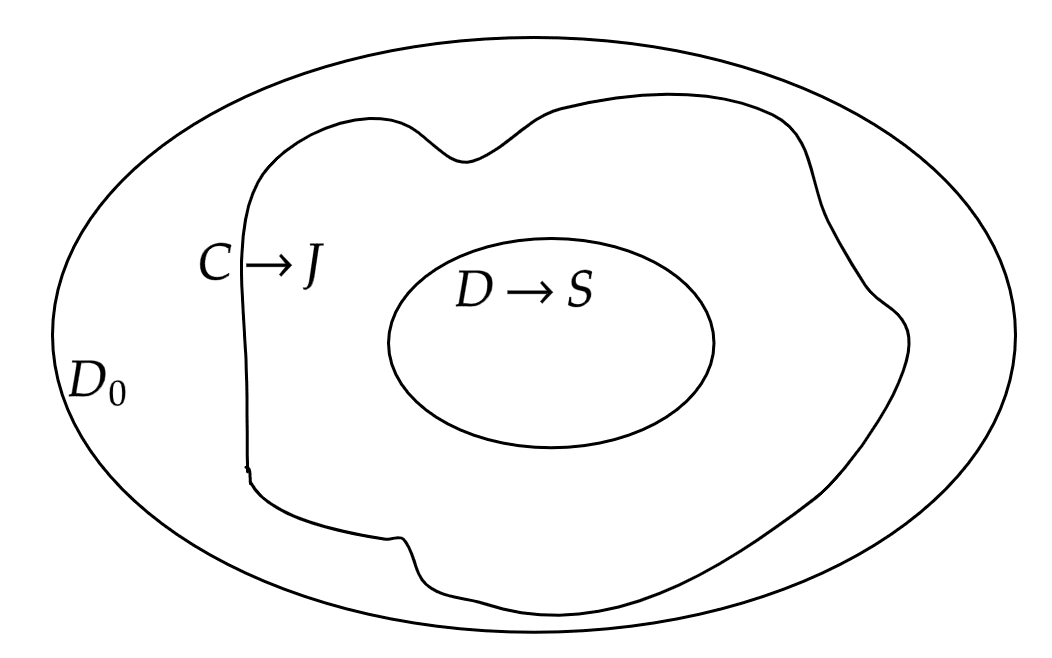
\includegraphics[width=0.5\textwidth]{Figs/13.png}
    % \caption{$\epsilon-\delta$ definition of stability.}
    % \label{fig:stabepsilon_delta}
\end{figure}

$\bullet$ \tb{differential $r$-form}

A differential $r$-form on an open set $E$ is a formal expression
\begin{align*}
\omega=\sum_{i_{1}=1}^{d} \ldots \sum_{i_{r}=1}^{d} p_{i_{1}} \ldots i_{r}(y) d y^{i_{1}} \wedge \cdots \wedge d y^{i_{r}}
\end{align*}
with real-valued coefficients defined on $E$.
\begin{rema}Some notes:
\begin{enumerate}
\item  $p_{i_{1}} \ldots i_{r}(y)=\pm p_{j_{1}} \ldots_{r}(y)$ according as $\left(j_{1}, \ldots, j_{r}\right)$ is an even or odd permutation of $\left(i_{1}, \ldots, i_{r}\right)$. In particular, $p_{i_{1} \ldots i_{r}}(y)=0$ if two of the indices $i_{1}, \ldots, i_{r}$ are equal. 
    \item Differential $r$-forms can be added in the obvious way. Differential $r$-and $s$-forms can be multiplied to give an $(r+s)$-form by the usual associative, distributive laws and anticommutative law $d y^{i} \wedge d y^{j}=-d y^{j} \wedge d y^{i}$.
\end{enumerate}
\end{rema}
\begin{defa}\bfs{Continuous or Class $C^{m}$ $k$-form}
The form $\omega$ is called continuous [or of class $C^{m}$ or 0 ] if its coefficients are continuous [or of class $C^{m}$ or identically 0] on $E$. 
\end{defa}

\begin{defa}\bfs{Uniformly Bounded [or Uniformly Convergent] $C^{m}$ $k$-form}
A sequence of differential $r$-forms on $E$ is said to be \tb{uniformly bounded [or uniformly convergent]} if the sequences of the corresponding coefficients are uniformly bounded [or uniformly convergent]. 
\end{defa}


\begin{defa}\bfs{Continuous Exterior Derivative} 
A continuous linear differential form ( $1$-form or Pfaffian)
\begin{align}
\omega=\sum_{j=1}^{d} p_{j}(y) d y^{j}\label{eq:5.1v}
\end{align}
on $E$ is said to possess a \tb{continuous exterior derivative} $d\omega$ if there exists a continuous differential $2$-form
\begin{align}
d \omega=\sum_{i=1}^{d} \sum_{j=1}^{d} p_{i j}(y) d y^{i} \wedge d y^{j}, \quad p_{i j}=-p_{ji}\label{eq:5.2v}
\end{align}
on $E$ such that Stokes' formula
\begin{align}
\int_{J} \omega=\iint_{S} d \omega\label{eq:5.3v}
\end{align}
holds for \tb{every piece} of $C^{1}$ surface $S$ in $E$ bounded by a $C^{1}$ piecewise Jordan curve $J$ in $E$.
\end{defa}
\begin{rema}\bfs{equivalent statement}
It is clear that if $S$ is the image of $D$ on the surface $S_{0}: y=y(u, v)$ for $(u, v) \in D$, and $J$ is the image of the Jordan curve $C$, then \cref{eq:5.3v} means that 
\begin{align}
    \int_{C} \sum_{j=1}^{d} p_{j}(y(u, v)) d y^{j}(u, v)=\int_{D} \sum_{i=1}^{d} \sum_{j=1}^{d} p_{i j}(y(u, v)) \frac{\partial\left(y^{i}, y^{j}\right)}{\partial(u, v)} d u d v \label{eq:5.4v}
\end{align} with the usual convention as to orientation of $C$ around $D$.
\end{rema}


\begin{exma}
If the coefficients $p_{j}(y)$ of \cref{eq:5.1v} are of class $C^{1}$, then $\omega$ has a continuous exterior derivative with $d \omega=\Sigma d p_{j}(y) \wedge d y^{j}$ or
\begin{align*}
d \omega=\sum_{i=1}^{d} \sum_{j=1}^{d} \frac{1}{2}\left(\frac{\partial p_{j}}{\partial y^{i}}-\frac{\partial p_{i}}{\partial y^{j}}\right) d y^{i} \wedge d y^{j} .
\end{align*}
\end{exma}

% There are cases, however, where \cref{eq:5.1v} has a continuous exterior derivative when the coefficients of \cref{eq:5.1v} are only continuous. Consider, for example, the case that there exists a real-valued function $U(y)$ of class $C^{1}$ such that $\omega=d U$ [i.e., $\left.p_{j}(y)=\partial U / \partial y^{j}\right]$, then $\omega$ has the exterior derivative $d \omega=0$. 

The fundamental lemma about the existence of continuous exterior derivatives is the following:
\begin{lema}
Let \cref{eq:5.1v} be a continuous linear differential $1$-form on an open set $E$. Then \cref{eq:5.1v} has a continuous exterior derivative \cref{eq:5.2v}  on $E$ if and only if, on every open subset $E^{0}$ with compact closure $E^{0} \subset E$, there exists a sequence of 1-forms $\omega^{1}, \omega^{2}, \ldots$ of class $C^{1}$ such that 
\begin{enumerate}
    \item $\omega^{n} \rightarrow \omega$ as $n \rightarrow \infty$ uniformly on $E^{0}$, and
    \item  $d \omega^{1}, d \omega^{2}, \ldots$ is uniformly convergent on $E^{0}$ %(in which case, $d \omega^{n} \rightarrow d \omega$ uniformly on $E^{0}$ as $\left.n \rightarrow \infty\right)$.
\end{enumerate}
\end{lema}
\begin{proof}
\tb{proof of ``$\Leftarrow$'':} Denote the limit of $d \omega^{n}$ as $d \omega$. For any $p_i$ as in \cref{eq:5.4v}, from uniform convergence and the exchange of integral and limit, we could get \cref{eq:5.3v}.

\tb{proof of ``$\Rightarrow$'':} If \cref{eq:5.1v} is a continuous 1-form on $E$ with a continuous exterior derivative \cref{eq:5.2v}, approximate the coefficients of $\omega$, $d\omega$ by the method in \cref{sec:smooth_app}: 

Let $\varphi(t)$ be as in \cref{sec:smooth_app} and put, for $\epsilon=1 / n$,
\begin{align*}
\begin{aligned}
&p_{i}^{(n)}(y)=c \epsilon^{-d} \int_{-\infty}^{+\infty} \ldots \int_{-\infty}^{+\infty} p_{i}(y-\eta) \varphi\left(\epsilon^{-2}\|\eta\|^{2}\right) d \eta^{1} \ldots d \eta^{d} \\
&p_{i j}^{(n)}(y)=c \epsilon^{-d} \int_{-\infty}^{\infty} \ldots \int_{-\infty}^{\infty} p_{i j}(y-\eta) \varphi\left(\epsilon^{-2}\|\eta\|^{2}\right) d \eta^{1} \ldots d \eta^{d} .
\end{aligned}
\end{align*}
Since the integrals are actually integrals over spheres $\|\eta\| \le \epsilon, p_{i}^{(n)}$ and $p_{i j}^{(n)}$ are defined on the sets $E_{n}$ consisting of points $y$ whose (Euclidean) distance from the boundary of $E$ not exceeds $\epsilon=1 / n$. In particular, they are defined on $E^{0}$ for large $n$ and tend uniformly to $p_{i}, p_{i j}$, respectively, on $E^{0}$, as $n \rightarrow \infty$.

Define the $C^{\infty}$ forms $\omega^{n}=\Sigma p_{j}^{(n)}(y) d y^{j}$ and $\alpha^{n}=\Sigma \Sigma p_{i j}^{(n)}(y) d y^{i} \wedge d y^{j}$ on $E^{0}$ for large $n$. Let $S$ be a piece of $C^{1}$ surface in $E^{0}$ bounded by a $C^{1}$ piecewise Jordan curve $J$ in $E^{0}$. Then if $\epsilon=1 / n$ is sufficiently small and $\|\eta\| \le \epsilon$, the translation $S(\eta)$ of $S$ by the vector $-\eta$ is in $E$ and \cref{eq:5.3v} is valid if $S$ is replaced by $S(\eta)$. This can be written in a form analogous to \cref{eq:5.4v},
\begin{align*}
\int_{C} \sum p_{j}(y(u, v)-\eta) d y^{j}(u, v)=\iint_{D} \sum \sum p_{i j}(y(u, v)-\eta) \frac{\partial\left(y^{i}, y^{j}\right)}{\partial(u, v)} d u d v
\end{align*}
Let this relation be multiplied by $c \epsilon^{-d} \varphi\left(\epsilon^{-2}\|\eta\|^{2}\right)$ and integrated over $\|\eta\| \le \epsilon$ with respect to $d \eta^{1} \ldots d \eta^{d} .$ An obvious change of the order of integration shows that the result can be interpreted as the Stokes' relation $\int_{J} \omega^{n}=\iint_{S} \alpha^{n} .$ Thus $\omega^{n}$ has the continuous exterior derivative $d \omega^{n}=\alpha^{n}$ in $E_{0}$. This completes the proof.
\end{proof}

In deciding whether or not a continuous 1 -form \cref{eq:5.1v} has the continuous exterior derivative \cref{eq:5.2v}, it suffices to verify Stokes' formula \cref{eq:5.3v} for rectangles $S$ on coordinate 2-planes $y^{i}=$ const. for $i \neq j, k$, where $1 \le j<k \le d$. This is a consequence of the following lemma.
\begin{lema}
A continuous differential $1$-form \cref{eq:5.1v} on an open set $E$ has a continuous exterior derivative.
\begin{enumerate}
    \item if and only if there exists a continuous differential $2$-form \cref{eq:5.2v} such that for every pair $j, k(1 \le j<k \le d)$ and fixed $y^{i}$, with $i \neq j, i \neq k$, the $1$-form $p_{j}(y) d y^{j}+p_{k}(y) d y^{k}$ has the continuous exterior derivative $p_{j k} d y^{j} \wedge d y^{k}+p_{k j} d y^{k} \wedge d y^{j}$; in other words, 
    \item if and only if Stokes' formula \cref{eq:5.3v} holds for all rectangle $S$ on 2-planes $y^{i}=$ const. for $i \neq j, k$ with closure $\bar{S} \subset E$.
\end{enumerate}
\end{lema}
\begin{proof}
I think the proof is based on the composition of the integration trail.
\end{proof}

$\bullet$  \tb{Notation}

For the sake of brevity, "vector" and "matrix" notation will be used in connection with $1$-forms and their exterior derivatives. For example, an ordered set of $e$ $1$-forms $\omega_{1}, \ldots, \omega_{e}$ will be abbreviated $\omega=\left(\omega_{1}, \ldots\right.$, $\left.\omega_{e}\right) ;$ analogously if these forms have continuous exterior derivatives, $d \omega$ denotes the ordered set of 2 -forms $d \omega=\left(d \omega_{1}, \ldots, d \omega_{e}\right)$. Finally, if $A=\left(a_{i j}(y)\right)$ is an $e \times d$ matrix function on $E$, by $\omega=A(y) d y$ will be meant the ordered set of 1-forms $\omega=\left(\omega_{1}, \ldots, \omega_{e}\right)$, where $\omega_{i}=$ $\sum_{j=1}^{d} a_{i j}(y) d y^{j}$ for $i=1, \ldots, e$.

\subsection{Another Difierentiability Theorem}
The main result \cref{thm:Peanodiff} on the differentiability of general solutions has the following generalization.

\begin{thma}\label{thm:jndnca}
   Let $f(t, y, z)$ be continuous on an open $(t, y, z)$-set $E$. %necessary and sufficient condition that t
   The initial value problem
\begin{align*}
y^{\prime}=f(t, y, z), \quad y\left(t_{0}\right)=y_{0}
\end{align*}
have a unique solution $y=\eta\left(t, t_{0}, y_{0}, z\right)$ for all $\left(t_{0}, y_{0}, z\right) \in E$ which is of class $C^{1}$ with respect to $\left(t, t_{0}, y_{0}, z\right)$ on its domain of definition \tb{if and only if} every point of $E$ have an open neighborhood $E^{0}$ on which there exist a \tb{continuous nonsingular} $d \times$ d matrix $A(t, y, z)$ and a continuous $d \times$ e matrix $C(t, y, z)$ such that the d differential 1-forms
\begin{align}
\omega=A(d y-f d t)+C d z\label{eq:6.2bb}
\end{align}
in the variables $d t, d y^{1}, \ldots, d y^{d}, d z^{1}, \ldots, d z^{e}$ have continuous exterior derivatives on $E^{0}$.
\end{thma}
\begin{rema}\bfs{compare with \cref{thm:Peanodiff} and more explanation}
In contrast to \cref{thm:Peanodiff}, the conditions of \cref{thm:jndnca} are invariant under $C^{1}$ changes of the variables $t, y, z$.

It is understood that if $A=\left(a_{i j}(t, y, z)\right)$ and $C=\left(c_{i k}(t, y, z)\right)$, then \cref{eq:6.2bb} represents an ordered set of 1 -forms, the $i$-th one of which is
\begin{align*}
\omega_{i}=\sum_{j=1}^{d} a_{i j} d y^{j}-\left(\sum_{k=1}^{d} a_{i j} f^{k}\right) d t+\sum_{k=1}^{e} c_{i k} d z^{k}
\end{align*}
$i=1, \ldots, d .$ If this has a continuous exterior derivative, the latter is a differential 2 -form of the type
\begin{align}
    d \omega_{i}=\sum_{j=1}^{d} \sum_{k=1}^{d} \alpha_{i j k} d y^{j} \wedge & d y^{k}+\sum_{j=1}^{d} \beta_{i j} d t \wedge d y^{j}+\sum_{k=1}^{e} \gamma_{i k} d t \wedge d z^{k}\nn
    &+\sum_{j=1}^{d} \sum_{k=1}^{e} \delta_{i j k} d z^{k} \wedge d y^{j}+\sum_{j=1}^{e} \sum_{k=1}^{e} \epsilon_{i j k} d z^{j} \wedge d z^{k}
\end{align}
where $\alpha_{i j k}=-\alpha_{i k j}, \beta_{i j}, \gamma_{i k}, \delta_{i j k}, \epsilon_{i j k}=-\epsilon_{i k j}$ are continuous function of $(t, y, z) .$ 
\end{rema}

% (6.6)
\cref{thm:jndnca} will be proved later. The proof of \cref{thm:jndnca}  will have the following consequence.
\begin{defa}
Define a $d \times d$ matrix $F(t, y, z)=\left(f_{i j}(t, y, z)\right)$ and a $d \times e$ matrix $N(t, y, z)=\left(n_{i j}(t, y, z)\right)$ by
\begin{align*}
\begin{aligned}
&f_{i j}=\beta_{i j}-2 \sum_{k=1}^{d} \alpha_{i j k} f^{k} \\
&n_{i j}=\gamma_{i j}+\sum_{k=1}^{d} \delta_{i k j} f^{k}
\end{aligned}
\end{align*}
\end{defa}

\begin{cora}
 Let $f(t, y, z)$ be as in \cref{thm:jndnca}, let $A(t, y, z), C(t, y, z)$ exist on $E^{0}$ as specified, and consider only $(t, y, z) \in E^{0} .$ Then $x=\partial \eta / \partial y_{0}^{k}$ is the solution of
\begin{align}
[A(t, \eta, z) x]^{\prime}=F(t, \eta, z) x, \quad x\left(t_{0}\right)=e_{k}\label{eq:6.7bb}
\end{align}
and $x=\partial \eta / \partial z^{i}$ is the solution of
\begin{align}
    \left[A(t, \eta, z) x+c_{i}(t, \eta, z)\right]^{\prime}=F(t, \eta, z) x+n_{i}(t, \eta, z), \quad x\left(t_{0}\right)=0,\label{eq:6.8bb}
\end{align}
where $c_{i}(t, y, z), n_{i}(t, y, z)$ are the $i$-th columns of $C(t, y, z), N(t, y, z)$, respectively, for $i=1, \ldots$, e and $\eta=\eta\left(t, t_{0}, y_{0}, z\right)$.
\end{cora} 
\begin{rema}
Note that a solution $x=x(t)$ of \cref{eq:6.7bb} does not necessarily have a derivative, but $A(x, \eta, z) x(t)$ has a derivative satisfying \cref{eq:6.7bb}. %An obvious change of variables reduces the linear equations in \cref{eq:6.7bb} and \cref{eq:6.8bb} to the type considered in Chapter IV; cf. (11.1)-(11.3).
\end{rema}

\begin{rema}\bfs{equivalent statement}
The statements concerning \cref{eq:6.7bb} and \cref{eq:6.8bb} can be written more conveniently as matrix equations
\begin{align}
    \left[A(t, \eta, z) \frac{\partial \eta}{\partial y_{0}}\right]^{\prime}=F(t, \eta, z) \frac{\partial \eta}{\partial y_{0}}, \quad \frac{\partial \eta}{\partial y_{0}}=I\text{ at }t=t_{0}
\end{align}
\begin{align}
    \left[A(t, \eta, z) \frac{\partial \eta}{\partial z}+C(t, \eta, z)\right]^{\prime}=F(t, \eta, z) \frac{\partial \eta}{\partial z}+N(t, \eta, z), \quad \frac{\partial \eta}{\partial z}=0\text{ at }t=t_{0}
\end{align}
\end{rema}


\bibliographystyle{IEEEtran}
\bibliography{IEEEabrv,StringDefinitions,adv_dnn}
\end{document}